\documentclass[12pt,a4paper]{book}
\usepackage[utf8]{inputenc}
\usepackage[portuguese]{babel}
\usepackage[T1]{fontenc}
\usepackage{amsmath}
\usepackage{amsfonts}
\usepackage{amssymb}
\usepackage{multicol}
\usepackage{graphicx}
\usepackage{wrapfig}
\usepackage{tikz}
%Serve para alterar o tipo de marcaçao no enumerate.
\usepackage{enumerate}
%o pacote e o comando abaixo servem para configurar as margens do documento.
\usepackage{geometry}
%se o pacote acima não for inserido, o comando abaixo não funciona.
\geometry{a4paper, left=2cm,right=2cm,bottom=2cm,top=2cm,headsep=1cm}
\title{Banco de Questões}
\date{Abril de 2015 \thanks{Última compilação: \today}}
\author{Arthur Astolfi Tótola}
\begin{document}	
	\maketitle
	\tableofcontents
	\newcounter{quest}
	%Data da última atualização: 04/11/2016

\chapter{Problemas para o 6º ano}
\section{As Quatro Operações}
\subsection{Adição}

\begin{list}{\textbf{Questão \arabic{quest}.}}{\usecounter{quest}}
%define a margem da lista.	
%\setlength{\labelwidth}{-2mm} \setlength{\parsep}{0mm}
%\setlength{\topsep}{0mm} \setlength{\leftmargin}{-2mm}
\renewcommand{\labelenumi}{(\alph{enumi})}

\item Calcule as somas
\begin{multicols}{4}
\begin{enumerate}[a)]
	\item 10 + 11 = 21
	\item 10 + 21 = 31
	\item 10 + 31 = 41
	\item 10 + 41 = 51
	\item 10 + 51 = 61
	\item 10 + 61 = 71
	\item 10 + 71 = 81
	\item 10 + 81 = 91
	\item 10 + 91 = 101
	\item 12 + 66 = 78
	\item 13 + 48 = 61
	\item 67 + 89 = 156
	\item 97 + 89 = 186
	\item 56 + 87 = 143
	\item 84 + 77 = 161
	\item 38 + 98 = 136
	\item 69 + 73 = 142
	\item 83 + 99 = 182
	\item 73 + 37 = 110
	\item 75 + 23 = 98
	\item 37 + 67 = 104
	\item 88 + 88 = 176
	\item 99 + 99 = 198
\end{enumerate}
\end{multicols}

\item calcule as somas

\begin{multicols}{4}
\begin{enumerate}[a)]
	\item 110 + 100 
	\item 120 + 101 
	\item 130 + 111 
	\item 140 + 121 
	\item 150 + 131 
	\item 170 + 132 
	\item 180 + 134 
	\item 190 + 135 
	\item 200 + 136
	\item 201 + 137 
	\item 210 + 138 
	\item 220 + 139
	\item 230 + 140 
	\item 240 + 150 
	\item 250 + 160 
	\item 260 + 170 
	\item 270 + 180
	\item 280 + 190
	\item 290 + 200
	\item 311 + 212
	\item 548 + 645
	\item 665 + 912
	\item 987 + 789
\end{enumerate}
\end{multicols}

\item Efetue as adições

\begin{multicols}{4}
\begin{enumerate}[a)]
	\item 1487 + 2365
	\item 6547 + 5478
	\item 4589 + 4587
	\item 3258 + 9632
	\item 7896 + 5697
	\item 5423 + 8912
	\item 7463 + 9641
	\item 2536 + 5847
	\item 7788 + 9988
	\item 1122 + 4477
	\item 7946 + 3146
	\item 4562 + 3215
	\item 1478 + 8632
	\item 8437 + 2791
	\item 2491 + 8461
	\item 6258 + 6412
	\item 5353 + 7887
	\item 3226 + 9558
	\item 1112 + 9994
	\item 6537 + 4538
	\item 2197 + 8617
	\item 1002 + 9913
	\item 9999 + 8888
\end{enumerate}
\end{multicols}

\item Efetue as adições

\begin{multicols}{2}
\begin{enumerate}[a)]
	\item 296 + 1634 + 98
	\item 109 + 432 + 7482
	\item 48 + 16409 + 287
	\item 31 + 1487 + 641 + 109
	\item 3412 + 1246
\end{enumerate}
\end{multicols}

\item Determine a soma do número 273 com o seu sucessor

\item Um objeto custa R\$ 415.720,00. O comprador terá ainda R\$ 28.912,00 de despesa de frete. Quanto o comprador vai pagar?

\item Ao receber o meu salário paguei R\$ 437,12 de aluguel, R\$ 68,14 de impostos, R\$ 1.089,67 de gastos com alimentação e ainda me sobraram R\$ 749,18. Quanto recebi de salário?

\item Um menino estuda 2 horas e 45 minutos pela manhã e 4 horas e 30 minutos à tarde. Quantos minutos estuda diariamente?

\item Um automóvel passou pelo quilômetro 435 de uma rodovia. Ele ainda deverá percorrer 298 quilômetros até chegar ao seu destino. Quantos quilômetros da estrada vai percorrer para chegar ao destino?

\item Em 1990 o Brasil vendeu para o exterior 283.356 veículos e, em 1991, essa venda foi de 345.760 veículos. Quantos veículos o Brasil vendeu para o exterior nesses dois anos?

\item Uma empresa tem sede em São Paulo e filiais em outros estados. Na sede trabalham 316 pessoas e nas filiais 1098 pessoas. Quantas pessoas trabalham nessa empresa?

\item Em um condomínio, há 675 lotes já vendidos e 1095 lotes para vender. Quantos lotes de terreno há nesse condomínio?

\item Uma escola funciona em dois turnos. No turno matutino há 1407 alunos e no turno vespertino há 1825 alunos. Quantos alunos estudam nessa escola?

\item Uma empresa produziu no primeiro trimestre 6905 peças. no segundo trimestre, a mesma empresa produziu 795 peças a mais que no primeiro trimestre. Nessas condições:
\begin{enumerate}
	\item Quantas peças a empresa produziu no segundo trimestre?
	\item Quantas peças a empresa produziu no semestre?
\end{enumerate}

\item Nei comprou um aparelho de som por 635 reais e as caixas de som por 128 reais. Tendo pago 12 reais pela instalação, qual a quantia que ele gastou ?

\item De acordo com o censo realizado em 1991, o estado da Paraíba tem 1.546.042 homens e 1.654.578 mulheres. Qual é a população da Paraíba segundo esse censo?

\item Calcule:

\begin{multicols}{3}
\begin{enumerate}[a)]
	\item 1705 + 395 
	\item 11.048 + 9.881 
	\item 4.907 + 62.103 
	\item 275.103 + 94.924 
	\item $545 + 2.298 + 99$
	\item $7.502 + 209.169 + 38.425$
\end{enumerate}
\end{multicols}

\end{list}

\subsection{Subtração}
\begin{list}{\textbf{Questão \arabic{quest}.}}{\usecounter{quest}}
%define a margem da lista.	
%\setlength{\labelwidth}{-2mm} \setlength{\parsep}{0mm}
%\setlength{\topsep}{0mm} \setlength{\leftmargin}{-2mm}
\renewcommand{\labelenumi}{(\alph{enumi})}

\item Calcule as subtrações
\begin{multicols}{3}
\begin{enumerate}[a)]
	\item 47 - 31
	\item 58 - 45
	\item 65 - 57
	\item 89 - 65
	\item 97 - 21
	\item 78 - 34
	\item 56 - 31
	\item 87 - 78
	\item 98 - 78
	\item 48 - 29
	\item 38 - 29
	\item 68 - 59
	\item 56 - 37
	\item 23 - 19
	\item 99 - 81
	\item 21 - 19
	\item 23 - 22
	\item 18 - 14
	\item 74 - 49
	\item 74 - 37
	\item 74 - 52
	\item 74 - 63
	\item 96 - 13
	 
\end{enumerate}
\end{multicols}

\item Calcule as Subtrações
\begin{multicols}{3}
\begin{enumerate}[a)]
	\item 72224 - 6458
	\item 701 - 638
	\item 131003 - 88043
	\item 1138 - 909
	\item 80469 - 6458
	\item 866 - 638
	\item 131012 - 88142
	\item 2238 - 909
	\item 802 - 638
\end{enumerate}
\end{multicols}

\item Dom Pedro II, imperador do Brasil, faleceu em 1891 com 66 anos de idade. Em que ano ele nasceu?

\item Um avião Boeing 747 pode transportar 370 passageiros e um avião DC-10 pode transportar 285 passageiros. Quantos passageiros o Boeing 747 pode transportar a mais que o DC-10?

\item À vista um automóvel custa 26.454 reais. À prazo o mesmo automóvel custa 38.392 reais. A diferença entre o preço cobrado é chamado de juros. Qual é a quantia que pagará de juros?

\item Um avião pode transportar 295 passageiros. Em determinado vôo, o avião está transportando 209 passageiros. Quantas poltronas desse avião não estão ocupadas?

\item Se Antônio tem 518 selos e Pedro tem 702 selos, Quantos selos Pedro tem a mais que Antônio?

\item Ézio tem 95 reais e quer comprar uma máquina fotográfica que custa 130 reais. Quantos reais faltam para ele comprar a máquina?

\item De acordo com o Censo de 1980, a população de uma cidade era de 79.412 habitantes. Feito o Censo em 1991, verificou-se que a população dessa cidade passou a ser de 94.070 habitantes. Qual foi o aumento da população dessa cidade nesse período de tempo?

\item Uma industria, no final de 1991, tinha 10.635 empregados. No inicio de 1992 em virtude da crise econômica dispensou 1.880 funcionários. Com quantos funcionários a indústria ficou?

\item Qual a diferença entre 10.000 e 5.995?

\item Quantas unidades faltam a 499 para atingir 1 unidade de milhar?

\item Efetue:
\begin{multicols}{4}
\begin{enumerate}[a)]
	\item 2620 - 945
	\item 7000 - 1096
	\item 11011 - 7997
	\item 140926 - 78016
\end{enumerate}
\end{multicols}

\item Considere os números 645 e 335. Nessas condições:
\begin{enumerate}[a)]
	\item Determine a diferença entre eles
	\item Adicione 5 unidades ao primeiro número e 5 unidades ao segundo número e calcule a diferença entre os novos números que você obteve. 
\end{enumerate}

\end{list}

\subsection{Multiplicação}

\begin{list}{\textbf{Questão \arabic{quest}.}}{\usecounter{quest}}
%define a margem da lista.	
%\setlength{\labelwidth}{-2mm} \setlength{\parsep}{0mm}
%\setlength{\topsep}{0mm} \setlength{\leftmargin}{-2mm}
\renewcommand{\labelenumi}{(\alph{enumi})}


\item Calcule as multiplicações
\begin{multicols}{4}
\begin{enumerate}[a)]
	\item 5 x 5 =
	\item 5 x 15
	\item 5 x 115
	\item 5 x 25 =
	\item 5 X 125 =
	\item 5 x 55 =
	\item 5 x 75 =
	\item 5 x 375 =
	\item 5 x 1257 =
	\item 6 x 5 =
	\item 6 x 15 = 
	\item 6 x 115 =
	\item 6 x 25 =
	\item 6 x 125 =
	\item 6 x 55 =
	\item 6 x 75 =
	\item 6 x 375 =
	\item 6 x 1257 =
	\item 7 x 5 =
	\item 7 x 15 =
	\item 7 x 115 =
	\item 7 x 25 =
	\item 7 x 125 =
	\item 7 x 55 =
\end{enumerate}
\end{multicols}

\item Calcule as multiplicações
\begin{multicols}{3}
\begin{enumerate}[a)]
	\item 7 x 75 =
	\item 7 x 375 =
	\item 7 x 1257 =
	\item 8 x 5 =
	\item 8 x 15 = 
	\item 8 x 115 =
	\item 8 x 25 =
	\item 8 x 125 =
	\item 8 x 55 =
	\item 8 x 75 =
	\item 8 x 375 =
	\item 8 x 1257 =
	\item 9 x 5 =
	\item 9 x 15 =
	\item 9 x 115 =
	\item 9 x 25 =
	\item 9 x 125 =
	\item 9 x 55 =
	\item 9 x 75 =
	\item 9 x 375 =
	\item 9 x 1257 =
	\item 9 x 999 =
	\item 9 x 123 =
\end{enumerate}
\end{multicols}

\item Efetue as Multiplicações
\begin{multicols}{3}
\begin{enumerate}[a)]
	\item 153 x 7 =
	\item 1007 x 9 =
	\item 509 x 62 =
	\item 758 x 46 =
	\item 445 x 93 =
	\item 289 x 140 =
	\item 1782 x 240 =
	\item 2008 x 405 =
	\item 2453 x 1002 =
\end{enumerate}
\end{multicols}

\item Efetue as multiplicações
\begin{multicols}{3}
\begin{enumerate}[a)]
	\item 28 x 0 =
	\item 49 x 10 =
	\item 274 x 10 =
	\item 158 x 100 =
	\item 164 x 1000 =
	\item 89 x 10000 =
\end{enumerate}
\end{multicols}

\item  Considerando 1 mês = 30 dias e 1 ano = 365 dias, uma semana = 7 dias, determine:
\begin{enumerate}[a)]
	\item quantos dias há em 15 semanas completas.
	\item Quantos dias há em 72 meses completos.
	\item Quantos dias há em 8 anos completos.
\end{enumerate}  

\item Para uma demonstração de ginástica, um professor de Educação Física prepara 64 grupos de alunos. Cada grupo é formado por 25 alunos. Quantos alunos devem participar dessa demostração?

\item Com 12 prestações mensais iguais de 325 reais posso comprar uma moto. Quanto vou pagar por essa moto? R: 3900 reais

\item Qual é o número natural que você vai obter quando multiplicar 736 por 208?

\item  Para cobrir o piso de um barracão foram colocados 352 placas de 35 metros quadrados cada uma. Quantos metros quadrados tem o piso desse barracão?

\item Um carro bem regulado percorre 12 quilômetros com um litro de gasolina. Se numa viagem foram consumidos 46 litros, qual a distância em quilômetros que o carro percorreu? 

\item Em um teatro há 18 fileiras de poltronas. Em cada fileira foram colocadas 26 poltronas. Quantas poltronas há nesse teatro? 
.
\item Em uma multiplicação, os fatores são 134 e 296. Qual o produto?

\item Numa mercearia há 7 caixas de bombons e cada caixa contém 3 duzias de bombons. Quantos bombons há na mercearia? 

\item Uma pessoa deu R\$ 4.700,00 de entrada na compra de um objeto e pagou mais 6 prestações de R\$ 2.300,00. Quanto custou o objeto?

\item Um motorista percorreu 749 km em 6 dias. Nos cinco primeiros dias andou 132 km por dia. Quanto percorreu no 6º dia ?

\item Calcule:
\begin{multicols}{3}
\begin{enumerate}[a)]
	\item 19 x 6 =
	\item 46 x 12 =
	\item 321 x 11 =
	\item 329 x 25 =
	\item 1246 x 24 =
	\item 67632 x 101 =
\end{enumerate}
\end{multicols}

\item Calcule as contas:
\begin{multicols}{3}
\begin{enumerate}[a)]
	\item 18 x 5 x 2 =
	\item 5 x 2 x 24 =
	\item 2 x 5 x 44 =
	\item 37 x 2 x 5 =
	\item 12 x 4 x 5 =
	\item 4 x 5 x 15=
\end{enumerate}
\end{multicols}

\item Em um banheiro tem uma parede com 15 fileiras com 10 azulejos e outra parede com 13 fileiras com 10. Quantos azulejos têm no banheiro? 

\item  Qual é o resultado da multiplicação de 63 por 12? 

\end{list}

\subsection{Divisão}

\begin{list}{\textbf{Questão \arabic{quest}.}}{\usecounter{quest}}
%define a margem da lista.	
%\setlength{\labelwidth}{-2mm} \setlength{\parsep}{0mm}
%\setlength{\topsep}{0mm} \setlength{\leftmargin}{-2mm}
\renewcommand{\labelenumi}{(\alph{enumi})}

\item Calcule as divisões
\begin{multicols}{3}
\begin{enumerate}[a)]
	\item 20:5=
	\item 16:8=
	\item 12:1=
	\item 48:8=
	\item 37:37=
	\item 56:14=
\end{enumerate}
\end{multicols}

\item Observe a igualdade $56\div 7=8$ e responda:
\begin{multicols}{2}
\begin{enumerate}[a)]
	\item Qual é o nome da operação?
	\item Como se chama o número 56?
	\item Como se chama o número 7?
	\item como se chama o número 8?
\end{enumerate}
\end{multicols}

\item Efetue as divisões
\begin{multicols}{3}
\begin{enumerate}[a)]
	\item 492:4= 
	\item 91:9=
	\item 4416:6=
	\item 2397:17=
	\item 1584:99=
	\item 1442:14=
	\item 21000:15=
	\item 7650:102=
	\item 11376:237=
\end{enumerate}
\end{multicols}

\item Responda
\begin{multicols}{2}
\begin{enumerate}[a)]
	\item Qual é a metade de 784?
	\item Qual é a terça parte de 144?
	\item Qual é a quinta parte de 1800?
	\item Qual é a décima parte de 3500?
\end{enumerate}
\end{multicols}

\item Em um teatro há 126 poltronas distribuídas igualmente em 9 fileiras. Quantas poltronas foram colocadas em cada fileira?

\item Quantos garrafões de 5 litros são necessários para engarrafar 315 litros de vinho?

\item Uma pessoa ganha R\$ 23,00 por hora de trabalho. Quanto tempo deverá trabalhar para receber R\$ 391,00?

\item Uma torneira despeja 75 litros de água por hora. Quanto tempo levará para encher uma caixa de 3150 litros ?

\item Numa pista de atletismo uma volta tem 400 metros. Numa corrida de 10.000 metros, quantas voltas o atleta tem de dar nessa pista?

\item Um livro tem 216 páginas. Quero terminar a leitura desse livro em 18 dias, lendo o mesmo número de páginas todos os dias. Quantas páginas preciso ler por dia?

\item Quantos grupos de 18 alunos podem ser formados com 666 alunos?

\item Uma tonelada de cana de açúcar produz aproximadamente 85 litros de álcool. Quantas toneladas de cana são necessárias para produzir 6970 litros de álcool?

\item Determine o quociente e o resto das seguintes divisões:
\begin{multicols}{3}
\begin{enumerate}[a)]
	\item 79:8= 
	\item 49:8= 
	\item 57:8= 
	\item 181:15= 
	\item 3214:10= 
	\item 825:18= 
	\item 4937:32= 
	\item 7902:12=
	\item 1545:114=
\end{enumerate}
\end{multicols}

\end{list}

\section{Problemas Envolvendo Adição e Subtração}
\begin{list}{\textbf{Questão \arabic{quest}.}}{\usecounter{quest}}
%define a margem da lista.	
%\setlength{\labelwidth}{-2mm} \setlength{\parsep}{0mm}
%\setlength{\topsep}{0mm} \setlength{\leftmargin}{-2mm}
\renewcommand{\labelenumi}{(\alph{enumi})}

	\item Resolva os problemas registrando todos os cálculos e a resposta de forma clara e completa.
	\begin{enumerate}[a)]
		\item Em uma escola de 612 alunos, 325 foram vacinados contra a gripe. Quantos alunos ainda precisam tomar a vacina? 
		\item Uma empresa de reciclagem de alumínio troca 1250 latas por um computador. A escola de Iara já juntou 763 latinhas. Quantas latinhas faltam para a escola de Iara ter a quantidade necessária para receber o computador?
		\item A diretora de uma escola organizou uma campanha de doação de livros para melhorar a biblioteca. Conseguiram 347 livros de doação e agora a biblioteca conta com 958 exemplares. Quantos livros a biblioteca tinha antes da campanha?
		\item José ficou muito confuso depois de bater figurinhas com Miguel. Tinham jogado duas partidas. José lembrava que na primeira partida ganhou 45 figurinhas e na segunda perdeu 52 figurinhas.Agora contava várias vezes as 63 figurinhas que ficaram em sua mão, sem se dar conta de quantas tinha antes de começar a jogar. Quantas figurinhas tinha José ao começar o jogo?
		\item No álbum de Ricardo cabem 356 figurinhas. Ele já colou 119. Quantas figurinhas Ricardo precisa colar para completar seu álbum?
		\item Mariana coleciona adesivos. No seu aniversário, ganhou 15 adesivos de seu avô e 6 de seu irmão. Como tinha alguns repetidos, deu 20 de presente a uma amiga que também coleciona adesivos, Como ficou a coleção de adesivos de Mariana? Ela ficou com mais ou com menos adesivos do que antes de seu aniversário: Quantos a mais ou quantos a menos?
		\item Hélio fez uma viagem de caminhão e abasteceu o tanque duas vezes, colocando 135 litros em cada parada. Durante toda a viagem consumiu 258 litros. Sobrou combustível no final da viagem? Justifique sua resposta.
		\item Embarcaram em um trem 420 pessoas na primeira estação. Na segunda estação subiram mais 130 pessoas e desceram 360. Na parada seguinte, desceram 340 pessoas e subiram 210. Quantas pessoas ficaram no trem após essas paradas?
		\item Um fazendeiro possui 524 bois. Na feira de gado vendeu 183 de seus bois e comprou outros 266 bois. Quantos bois o fazendeiro tem agora?
		\item Ana deve 315 reais para Paula e Paula deve 238 reais para Ana. Quem deve pagar a quem para saldar as dívidas? Quanto?
		\item Estou poupando para comprar uma bicicleta de R\$ 300,00. Minha mãe me deu R\$ 130,00, meu padrinho me presenteou com R\$ 82,00 e meu irmão mais velho me deu R\$ 25,00 em uma semana e R\$ 17,00 na outra . O que eu juntei dá para comprar a bicicleta? Sobra o falta? Quanto?
		\item Lucas nasceu em 1984. Quantos anos completará em 2020?		
	\end{enumerate}
	
	\item Sete amigos querem repartir 630 reais entre eles. Todos têm que receber a mesma quantia e não pode sobrar nada. Como podem fazer a divisão? Quanto cabe a cada um?
	\item A avó de Paula repartiu 56 reais igualmente entre seus netos de tal maneira que cada um recebeu 8 reais. Entre quantos netos ele repartiu o dinheiro?
	\item A professora do 5º ano repartiu 90 lápis de cor entre alguns alunos. Cada aluno recebeu 9 lápis. Quantos alunos receberam lápis de cor?
	\item Aílton quer plantar, em sua chácara, 45 limoeiros em 5 filas. Quantos limoeiros deve plantar em cada fileira?
	\item Uma padaria prepara 140 tortas todos dos dias. Para assá-las o padeiro coloca 8 tortas em cada bandeja. Quantas bandejas são necessárias para assar todas as tortas?
	
	\item Em uma campanha de vacinação a previsão era de que no mínimo 20 000 crianças fossem vacinadas em dois dias. No primeiro dia foram vacinadas 11 640 crianças e no segundo dia, 3 264 crianças a menos do que no dia anterior. Verifique se o objetivo foi alcançado.
	\item Na escola de Pedro há 8 classes de 35 alunos, 5 classes de 33 alunos e 12 classes de  30 alunos. Qual o total de alunos nessa escola?
	\item Fabrício tinha 320 reais para pagar as contas (117 reais de energia elétrica, 58 reais de água e 88 reais de telefone) e para fazer algumas compras. Quanto lhe restou para fazer as compras?
	\item Foram repartidas 45 balas entre três crianças: Raul e Mara receberam quantidades iguais e Paula recebeu 3 balas a mais do que Raul. Quantas balas recebeu cada criança?
	\item Numa gincana de perguntas e respostas o aluno ganhava 3 pontos por acerto e perdia 2 pontos a cada erro. Um aluno respondeu a 20 perguntas e ganhou 40 pontos. Quantos acertos e quantos erros ele teve?
	\item Mirtes tinha uma quantia no banco. Na segunda-feira retirou 135 reais e na terça-feira fez um depósito de 87 reias. Com isso, ficou com saldo de 344 reais. Quantos ela tinha no início?
	\item Tio Patinhas distribuindo 300 selos entre seus três sobrinhos, Luizinho, Huguinho e Zezinho, de modo que Huguinho recebeu 20 selos a mais do que Luizinho, e Zezinho recebeu 80 selos a mais do que Huguinho. Quantos selos cada um recebeu?
	
\item Comprei 20 livros e depois comprei mais 13. Quantos livros comprei ao todo?

	\item Ao pagar R\$ 400,00, liquidei uma dívida de R\$ 1000,00. Quanto já havia pago dessa dívida?

	\item Vovó recebeu 36 rosas. Uma dúzia foi mandada pelos netos e as outras pelos filhos. Quantas rosas mandaram os filhos? 

	\item Comprei 9 revistas. Já li 5. Quantas revistas ainda tenho para ler? 

	\item Gastei R\$ 500,00 do que possuía e ainda fiquei com R\$ 600,00. Quanto eu tinha?

	\item Que idade terá, em 2014 uma pessoa que nasceu em 1992?

	\item Recebi 20 quilos de uvas. Dei 6 quilos para meu irmão e 5 para um primo. Com quantos quilos de uva eu fiquei?

	\item Numa granja havia 132 galinhas num galinheiro e 40 em outro. O granjeiro vendeu 58 galinhas. Quantas galinhas ainda havia?

	\item No início do ano, uma classe da escola possuía um certo número de alunos. No final do 1º semestre saíram 10 alunos e no início do 2º semestre foram matriculados mais 8, totalizando, agora, 35 alunos. Quantos alunos havia nessa classe no início do ano?

	\item Uma professora recebeu vinte e cinco livros. Deu alguns para seus alunos e depois recebeu mais três livros, ficando com dezoito livros. Quantos livros a professora deu para seus alunos?	
	
	\item Um funcionário foi admitido numa empresa aos 14 anos e aposentou-se após 43 anos de trabalho. Qual a idade desse funcionário ao se aposentar?

	\item Um carro usado foi comprado por R\$ 3500,00 e vendido por R\$ 7150,00 após passar por reparos no valor de R\$ 2300,00. Qual o lucro obtido nessa venda?
	\item Um pasteleiro fez 89 pastéis de carne e 76 de queijo. Vendeu 135 pastéis. Quantos ainda não foram vendidos?

	\item Uma pessoa comprou uma casa por R\$ 60000,00. Gastou R\$ 75000,00 em reformas e vendeu com um lucro de R\$ 120000,00. Qual o preço de venda da casa?

	\item Uma biblioteca adquiriu livros de ciências, português e história. Os livros de história eram em números de três a mais que os de português e, estes, seis a mais que os de ciências. Qual a quantidade de livros adquirida se os livros de ciências eram vinte quatro?

	\item Napoleão Bonaparte nasceu em 1769 e morreu com 52 anos. Em que ano morreu?
\end{list}

%==================================================================================================
\section{Potenciação}
\begin{list}{\textbf{Questão \arabic{quest}.}}{\usecounter{quest}}
%define a margem da lista.	
%\setlength{\labelwidth}{-2mm} \setlength{\parsep}{0mm}
%\setlength{\topsep}{0mm} \setlength{\leftmargin}{-2mm}
\renewcommand{\labelenumi}{(\alph{enumi})}

\item Transforme os produtos indicados, em potência:
\begin{multicols}{3}
\begin{enumerate}[a)]
	\item $3\cdot 3 =$
	\item $6\cdot  6\cdot  6 =$
	\item $5\cdot  5\cdot  5 =$
	\item $2\cdot  2\cdot  2\cdot  2 =$
	\item $7\cdot  7 =$
	\item $45\cdot  45\cdot  45\cdot  45=$
	\item $8\cdot  8\cdot  8\cdot  8 =$
	\item $ 68\cdot  68\cdot  68\cdot  68\cdot  68\cdot  68=$
	\item $1\cdot  1\cdot  1\cdot  1\cdot  1\cdot  1\cdot  1 =$
	\item $ 89\cdot  89\cdot  89 =$
\end{enumerate}
\end{multicols}

\item Transforme em produto, as potências:
\begin{multicols}{3}
\begin{enumerate}[a)]
	\item $4^2=$
	\item $5^3=$
	\item $2^6=$
	\item $7^3$
	\item $3^4$
	\item $38^5$
	\item $7^6$
	\item $12^6$
	\item $20^3$	
\end{enumerate}
\end{multicols}

\item Escreva como se lê:
\begin{multicols}{5}
\begin{enumerate}[a)]
	\item $4^2=$
	\item $5^3=$
	\item $2^6=$
	\item $7^3$
	\item $3^4$
	\item $38^5$
	\item $7^6$
	\item $12^6$
	\item $20^3$
	\item $100^{100}$
\end{enumerate}
\end{multicols}

4) Indique que é a base, o expoente e calcule as seguintes potências:
\begin{multicols}{5}
\begin{enumerate}[a)]
	\item $4^2=$
	\item $5^ 3=$
	\item $2^6=$
	\item $7^3=$
	\item $3^4=$
	\item $38^1=$
	\item $17^0=$
	\item $12^2=$
	\item $0^4=$
	\item $20^3$
\end{enumerate}
\end{multicols}

\item Calcule:
\begin{multicols}{6}
\begin{enumerate}[a)]
	\item $2^3 =$
	\item $3^5 =$
	\item $1^2 =$
	\item $1^3 =$
	\item $10^3 =$
	\item $3^2 =$
	\item $4^2 =$
	\item $2^1 =$
	\item $3^1 =$
	\item $4^3 =$
	\item $0^4 =$
	\item $5^0 =$
	\item $3^0 =$
	\item $1^7 =$
	\item $6^0 =$
	\item $10^5 =$
	\item $1^4 =$
	\item $4^1 =$
\end{enumerate}
\end{multicols}

\item Escreva as potências com os números naturais e depois resolva:
\begin{enumerate}[a)]	
	\item Dezesseis elevado ao quadrado
	\item Cinquenta e quatro elevado à primeira potência	
	\item Zero elevado à décima primeira potência
	\item Um elevado à vigésima potência
	\item Quatorze elevado ao cubo
	\item Dois elevado à nona potência
	\item Três elevado à quarta potência
	\item Dez elevado à sexta potência
	\item Oitenta e cindo elevado a zero
	\item Dois mil e quarenta e seis elevado à primeira potência
\end{enumerate}

Nos testes a seguir assinale a alternativa correta:
\item Na potenciação sempre que a base for 1 a potência será igual a:
\begin{enumerate}[a)]
	\item 1
	\item 0
	\item Expoente natural
	\item 10
	\item N.d.a. (nenhuma destas alternativas)
\end{enumerate}

\item Todo número natural não-nulo elevado à zero é igual a:
\begin{enumerate}[a)]
	\item Ele mesmo
	\item 0
	\item 1
	\item 10
	\item N.d.a
\end{enumerate}

\item Qual o resultado de $4^3$ ?
\begin{enumerate}[a)]
	\item 13
	\item 63
	\item 56
	\item 64
	\item 24
\end{enumerate}

\item Todo número natural elevado a 1 é igual a:
\begin{enumerate}[a)]
	\item 0
	\item Ele mesmo
	\item 1
	\item 10
	\item N.d.a
\end{enumerate}
\end{list}

\section{Expreções Numéricas}
\subsection{Expressões Com Adição e Subtração}
\begin{list}{\textbf{Questão \arabic{quest}.}}{\usecounter{quest}}
%define a margem da lista.	
%\setlength{\labelwidth}{-2mm} \setlength{\parsep}{0mm}
%\setlength{\topsep}{0mm} \setlength{\leftmargin}{-2mm}
\renewcommand{\labelenumi}{(\alph{enumi})}

	\item Calcule o valor das expressões
	\begin{multicols}{2}
	\begin{enumerate}[a)]
		\item $10-1+8-4=$
		\item $12-8+9-3=$
		\item $25-1-4-7=$
		\item $ 45-18+3+1-2=$
		\item $75-10-8+5-1=$
		\item $10+5-6-3-3+1=$
	\end{enumerate}
	\end{multicols}
	\item Efetue as operações
	\begin{multicols}{2}
	\begin{enumerate}[a)]
		\item $ 237+98 =$
		\item $648+2334 =$
		\item $4040+404 =$
		\item $4620+1398+27$
		\item $3712+8109+105+79 =$
		\item $256-84 =$
		\item $2711-348 =$
		\item $1768-999 =$
		\item $5043-2584 =$
		\item $ 8742-6193 =$
	\end{enumerate}
	\end{multicols}

	\item Calcule o valor das expressões
	\begin{multicols}{2}
	\begin{enumerate}[a)]
		\item $30-(5+3) = $
		\item $15+(8+2) =$
		\item $15-(10-1-3) =$
		\item $23-(2+8)-7 = $
		\item $(10+5)-(1+6) =$
		\item $ 7-(8-3)+1=$
	\end{enumerate}
	\end{multicols}
	\item Calcule o valor das expressões
	\begin{multicols}{2}
	\begin{enumerate}[a)]
		\item $25-[10+(7-4)] =$
		\item $32+[10-(9-4)+8] =$
		\item $45-[12-4+(2+1)] =$
		\item $70-\{20-[10-(5-1)]\} =$
		\item $28+\{13-[6-(4+1)+2]-1\} =$
		\item $53-\{20-[30-(15-1+6)+2]\} =$
		\item $62-\{16-[7-(6-4)+1]\} =$
		\item $20-\{8+[3+(8-5)-1]+6\} =$
		\item $15+\{25-[2-(8-6)]+2\} =$
		\item $56-[3+(8-2)+(51-10)-(7-2)] =$
		\item $\{42+[(45-19)-(18-3)+1]-(28-15)-1\} $
	\end{enumerate}
	\end{multicols}
	\item Calcule o valor da expressões
	\begin{multicols}{2}
	\begin{enumerate}[a)]
		\item $7-(1+3)=$
		\item $9-(5-1+2)=$
		\item $10-(2+5)+4=$
		\item $(13-7)+8-1=$
		\item $15-(3+2)-6=$
		\item $(10-4)-(9-8)+3=$
		\item $50-[37-(15-8)]=$
		\item $28+[50-(24-2)-10]=$
		\item $20+[13+(10-6)+4]=$
		\item $52-{12+[15-(8-4)]}=$
	\end{enumerate}
	\end{multicols}

	\item Calcule o valor das expressões:
	\begin{multicols}{2}
	\begin{enumerate}[a)]
		\item $25 + \{ 12 + [ 2 - ( 8 - 6 ) + 2 ]\} =$
		\item $\{ [ ( 18 - 3 ) + ( 7 + 5) - 2 ] + 5 \} - 12 =$
		\item $65 - \{ 30 - [ 20 - ( 10 - 1 + 6) + 1 ]\}= $
		\item $45 + \{ 15 - [ ( 10 - 8 ) + ( 7 - 4) - 3 ] - 4 \} =$
		\item $40 + \{ 50 - [35 - ( 25 +5) - 1 ]\} + 7 $
		\item $38 - \{ 20 - [ 22 - ( 5 + 3) + ( 7 - 4 +1)]\} =$
		\item $26 + \{ 12 - [ ( 30 - 18) + ( 4 - 1) - 6 ] - 1 \} =$
	\end{enumerate}
	\end{multicols}

	\item Calcule o valor das expressões
	\begin{multicols}{2}
	\begin{enumerate}[a)]
		\item $10 - 5 - 2 + 3 =$		
		\item $10 - ( 5 + 2) + 3 =$
		\item $( 10 - 5) - ( 2 + 3) =$
		\item $10 - ( 5 - 2 + 3) =$
		\item $( 17 + 9 ) - 8 - ( 11 + 4) = $
		\item $ 86 + ( 31 - 16 + 60 ) - ( 200 - 70 - 50 ) $
		\item $( 79 + 21 - 84) + ( 63 - 41 + 17 ) - 26 = $		
	\end{enumerate}
	\end{multicols}

	\item Calcule o valor das expressões:
	\begin{multicols}{2}
	\begin{enumerate}[a)]
		\item $10 - 1 + 8 - 4 = $				
		\item $12 - 8 + 9 - 3 = $	
		\item $25 - 1 - 4 - 7 =$	
		\item $30 - ( 5 + 3 ) =$	
		\item $15 + ( 8 + 2 ) =$	
		\item $25 - ( 10 - 1 - 3 ) =$	
		\item $45 - 18 + 3 + 1 - 2 =$	
		\item $75 - 10 - 8 + 5 - 1 =$				
		\item $10 + 5 - 6 - 3 - 3 + 1 =$	
		\item $23 - ( 2 + 8 ) - 7 =$	
		\item $( 10 + 5 ) - ( 1 + 6 ) =$	
		\item $7 - ( 8 - 3 ) + 1 =$	
		\item $25 - [ 10 + ( 7 - 4 ) ] = $				
		\item $32+ [ 10 - ( 9 - 4 ) + 8 ] =$	
		\item $45 - [ 12 - 4 + ( 2 + 1 )] =$	
		\item $70 - \{ 20 - [ 10 - ( 5 - 1 ) ]\} =$	
		\item $28 + \{ 13 - [ 6 - ( 4 + 1 ) + 2 ] - 1 \}=$	
		\item $53 - \{ 20 - [ 30 - ( 15 - 1 + 6 ) + 2 ]\} =$	
		\item $ 62 - \{ 16 - [ 7 - ( 6 - 4 ) + 1 ]\} =$
		\item $20 - \{ 8 + [ 3 + ( 8 - 5 ) - 1 ] + 6\} =$				
		\item $15 + \{ 25 - [ 2 - ( 8 - 6 )] + 2 \} = $	
		\item $56 - [ 3 + ( 8 - 2 ) + ( 51 - 10 ) + ( 7 - 2 )] =$	
		\item $\{ 42 + [ (45 - 19) - ( 18 - 3 ) + 1] - (28 - 15 )\}  =$	
		\item $ 7 - ( 1 + 3 ) =$	
		\item  $9 - ( 5 - 1 + 2 ) =$
		\item $10 - ( 2 + 5 ) + 4 =$	
	\end{enumerate}
	\end{multicols}
	
	\item Determine os valores das expressões numéricas.
	\begin{multicols}{3}
	\begin{enumerate}[a)]
		\item $7-2\cdot 3$
		\item $(7-2)\cdot 3$
		\item $8-7+1$
		\item $8-(7+1)$
		\item $6^2-\sqrt{36}$
		\item $\sqrt{100}:(2\cdot 5)$
	\end{enumerate}
	\end{multicols}
	\item Calcule o valor das expressão $10+(8-6:3)$.
	\item As expressões numéricas $\sqrt{36}+64$ e $\sqrt{36+64}$ têm o mesmo valor? Calcule o valor de cada uma.
	\item Mário comprou para seu filho um livro e dois cadernos e indicou a quantia total que gastou pela expressão $10+2\cdot 3$. Escreva a quantia que ele gastou.
	\item Calcule o valor de cada expressão numérica:
	\begin{multicols}{4}
	\begin{enumerate}[a)]
		\item $12:(3\cdot 4)$
		\item $12:3\cdot 4$
		\item $2\cdot \sqrt{49}$
		\item $3^2+2^3$
		\item $4+2\cdot 3-5$
		\item $(4+6):(3^2-7)$
		\item $2+\sqrt{9}\cdot 5$
		\item $14-5+2^4$
	\end{enumerate}
	\end{multicols}
	\item João Pessoa, na capital da Paraíba, é uma das cidades mais antigas de nosso país. O valor da expressão $10^2\times\sqrt{25}\times3+8^2 +21$ indica o ano em que essa cidade foi fundada. Em que ano João Pessoa foi fundada?
	\item Calcule o valor de cada uma das expressões numéricas:
	\begin{multicols}{2}
	\begin{enumerate}[a)]
		\item $\{2+[(3-1)\cdot (3+3):4\}$
		\item $4+\{8+2\cdot [3+(10+2\cdot 7):8]\}$
		\item $\{[(20:10\cdot 2)+5]:3\}+2^3$
		\item $\{2\cdot [7-(\sqrt{16}+1):5]:4\}^2$
		\item $(3^2-2^3)\cdot 3^3-2^3+2^2\cdot 4^2$
		\item $(\sqrt{5^4}-5^2):(6+12\cdot 2)$
	\end{enumerate}
	\end{multicols}
\end{list}

\subsection{Expressões Numéricas com as Quatro Operações}
\begin{list}{\textbf{Questão \arabic{quest}.}}{\usecounter{quest}}
%define a margem da lista.	
%\setlength{\labelwidth}{-2mm} \setlength{\parsep}{0mm}
%\setlength{\topsep}{0mm} \setlength{\leftmargin}{-2mm}
\renewcommand{\labelenumi}{(\alph{enumi})}

\item Calcule as expressões
\begin{multicols}{2}
\begin{enumerate}[a)]
	\item $3\cdot 75+3\cdot 25 =$
	\item $5\cdot 97+5\cdot 3 =$
	\item $4\cdot 101+4\cdot 99 =$
	\item $ 20\cdot 47+80\cdot 47 =$
	\item $12+16:8\cdot 3-5 =$
	\item $ 100-6\cdot 7+8:2 =$
	\item $64:8+5\cdot 5-3 =$
	\item $1+3+5\cdot 7-9:3 =$
\end{enumerate}
\end{multicols}

\item Calcule o valor das expressões:
\begin{multicols}{2}
\begin{enumerate}[a)]
	\item $ 7+15:3 =$
	\item $4\cdot 5+1 =$
	\item $10:2+8 = $
	\item $32+12:2 =$
	\item $20:10+10 =$
	\item $7\cdot 3-2\cdot 5 =$
	\item $40-2\cdot 4+5 =$
	\item $4\cdot 3+10:2 =$
	\item $50-16:8+7 =$
	\item $32:4:2:2 =$
\end{enumerate}
\end{multicols}

\item Calcule o valor das expressões
\begin{multicols}{2}
\begin{enumerate}[a)]
	\item $(13+2)\cdot 3+5 =$
	\item $(7+2)\cdot (3-1) =$
	\item $(4+2\cdot 5)-3 =$
	\item $ 20-(15+6:3) =$
	\item $15+[6+(8-4:2)] =$
	\item $40-[3+(10-2):2] =$
	\item $[30+2\cdot (5-3)]\cdot 2-10 =$
	\item $10+[4+(7\cdot 3+1)]-3 =$
\end{enumerate}
\end{multicols}


\item Calcule o valor das expressões
\begin{multicols}{2}
\begin{enumerate}[a)]
	\item $(3+2)\cdot (5-1)+4 =$
	\item $ 82-8\cdot 7:(4-1\cdot 3) =$
	\item $25-[10-(2\cdot 3+1)] $
	\item $70-[12+(5\cdot 2-1)+6] =$
	\item $8:2+[15-(4\cdot 2+1)] =$
	\item $9+[4+2\cdot (6-4)+(2+5)]-8 =$
	\item $50+\{10-2\cdot [(6+4:2)-(10-3)]\} =$
	\item $180:\{10+2\cdot [20-45:(13-2\cdot 5)]\} =$	
\end{enumerate}
\end{multicols}

\item Calcule o valor das expressões:
\begin{multicols}{2}
\begin{enumerate}[a)]
	\item $70:7-1=$
	\item $ 20+3\cdot 2=$
	\item $30+10:10 =$
	\item $ 150-7\cdot 12=$
	\item $48:16+20:4 =$
	\item $10-8:2+3 =$
	\item $ 30:5-1+2\cdot 3 =$
\end{enumerate}
\end{multicols}

\item Calcule as expressões:
\begin{multicols}{2}
\begin{enumerate}[a)]
	\item $(3+4)\cdot (9-8) =$
	\item $(20+8):(3+4) =$
	\item $15+8\cdot (2+3) =$
	\item $(5+3\cdot 2)-1=$
	\item $ 25+(8:2+1)-1= $
	\item $15+[5\cdot (8-6:2)] =$
	\item $50-[13-(10-2):2] =$
	\item $[40+2\cdot (7-5)]\cdot 2-20 $
\end{enumerate}
\end{multicols}

\item Calcule o valor das expressões:
\begin{multicols}{2}
\begin{enumerate}[a)]
	\item $16+[10-(18:3+2)+5] =$
	\item $25-[12-(3\cdot 2+1)] =$
	\item $90-[25+(5\cdot 2-1)+3] =$
	\item $45+[(8\cdot 5-10:2)+(18:6-2)] =$
	\item $50-2\cdot \{7+8:2-[9-3\cdot (5-4)]\}$
	\item $100-3\cdot \{5+8:2-[3\cdot (7-6)]\} =$
\end{enumerate}
\end{multicols}

\item Determine o valor de cada expressão
\begin{multicols}{2}
\begin{enumerate}[a)]
	\item $1000 - [(2 . 4 - 6) + ( 2 + 6 . 4)] =$
	\item $60 + 2 \cdot \{[ 4 \cdot ( 6 + 2 ) - 10 ] + 12\} =$
	\item $[( 4 + 16 \cdot 2) \cdot 5 - 10] \cdot 100 =$
	\item $\{ 10 + [ 5 \cdot ( 4 + 2 \cdot 5) - 8] \cdot 2 \} - 100 =$
	\item $80 - 5 \cdot ( 28 - 6 \cdot 4 ) + 6 - 3 \cdot 4 =$
\end{enumerate}
\end{multicols}

\item  Calcule
\begin{multicols}{2}
\begin{enumerate}[a)]
	\item $4 \cdot ( 10 + 20 + 15 + 30) =$
	\item $(10 \cdot 6 + 12 \cdot 4 + 5 \cdot 8 ) - 40 =$
	\item $[ 6 \cdot ( 3 \cdot 4 - 2 \cdot 5) - 4 ] + 3 \cdot ( 4 - 2) - ( 10 : 2 ) =$
	\item $67 + \{ 50 \cdot [ 70 : ( 27 + 8 ) + 18 : 2 ] + 21 \} =$
	\item $[ 30 \cdot ( 9 - 6)] + [ 30 : ( 9 + 6 ) ] =$
	\item $ 58 - [ 20 - ( 3 \cdot 4 - 2) : 5 ] =$
	\item $ 40 + 2 \cdot [ 20 - ( 6 + 4 \cdot 7 ) : 2 ] =$
\end{enumerate}
\end{multicols}

\item Calcule o valor das expressões
\begin{multicols}{2}
\begin{enumerate}[a)]
	\item $(12 + 2 \cdot 5) - 8 =$
	\item $25 - ( 15 + 6 : 3) =$
	\item $25 +[7 + ( 8 - 4 :2)] =$
	\item $60 - [8 + ( 10 - 2 ) : 2] =$
	\item $80 - [ 22 + ( 5 \cdot 2 - 1 ) + 6] $
	\item $14 : 2 + [ 13 - ( 4 \cdot 2 + 1 ) ] =$
	\item $[ 30 + 2 \cdot  ( 5 - 3 ) ] \cdot  2 - 10 =$
	\item $20 : 10 + 10 =$
	\item $10 + [ 4 + ( 7 \cdot  3 + 1 ) ] - 3 =$
\end{enumerate}
\end{multicols}

\item  Resolva as expressões numéricas:
\begin{multicols}{2}
\begin{enumerate}[a)]
	\item $8 - ( 1 + 3) =$
	\item $7\cdot  3 - 2 \cdot  5 =$
	\item $( 13 - 7 ) + 8 - 1 =$
	\item $4 \cdot  3 + 10 : 2 =$
	\item $15 - ( 3 + 2 ) - 6 =$
	\item $40 - 2 \cdot  4 + 5 =$
	\item $( 10 - 4 ) - ( 9 - 8 ) + 3 =$
	\item $50 - 16 : 8 + 7 =$
	\item $50 - [37 - ( 15 - 8 ) ] = $
	\item $ 32 : 4 : 2 : 2 =$
	\item $28 + [ 50 - ( 24 - 2 ) - 10 ] =$
	\item $( 13 + 2) \cdot  3 + 5 =$
	\item $20 + [ 13 + ( 10 - 6 ) + 4 ] =$
	\item $( 7 + 2 ) \cdot  ( 3 - 1 ) =$
	\item $52 - \{ 12 + [ 15 - ( 8 - 4 )]\}=$
	\item $( 4 + 2 \cdot  5 ) - 3 =$
	\item $7 + 15 : 3 =$
	\item $20 - ( 15 + 6 : 3) =$
	\item $4 \cdot  5 + 1 =$
	\item $15 + [ 6 + ( 8 - 4 : 2 )] =$
	\item $10 : 2 + 8 =$
	\item $40 - [ 3 + (10 - 2 ) : 2 ] =$
	\item $ 32 + 12 : 2 =$
\end{enumerate}
\end{multicols}
\end{list}

%=====================================================================================
\subsection{Expressões Numéricas com Potências}
\begin{list}{\textbf{Questão \arabic{quest}.}}{\usecounter{quest}}
%define a margem da lista.	
%\setlength{\labelwidth}{-2mm} \setlength{\parsep}{0mm}
%\setlength{\topsep}{0mm} \setlength{\leftmargin}{-2mm}
\renewcommand{\labelenumi}{(\alph{enumi})}

\item Calcule o valor das expressões:
\begin{multicols}{5}
\begin{enumerate}[a)]
	\item $7^2 - 4 =$
	\item $2^3 + 10 =$
	\item $5^2 - 6 =$
	\item $4^2 + 7^0=$
	\item $5^0+ 5^3=$
	\item $2^3+ 2^4 =$
	\item $10^3 - 10^2 =$
	\item $80^1 + 1^{80} =$
	\item $5^2 - 3^2 =$
	\item $1^{80} + 0^{70} =$
\end{enumerate}
\end{multicols}

\item Calcule:
\begin{multicols}{4}
\begin{enumerate}[a)]
	\item $3^2 + 5 =$
	\item $3 + 5^2 =$
	\item $3^2 + 5^2 =$
	\item $5^2 - 3^2 =$
	\item $18 - 7^0 =$
	\item $5^3 - 2^2 =$
	\item $10 + 10^2 =$
	\item $10^3 - 1^1 =$
\end{enumerate}
\end{multicols}

\item Calcule o valor das expressões
\begin{multicols}{3}
\begin{enumerate}[a)]
	\item $2^3 \cdot 5 + 3^2 =$
	\item $70^0+ 0^{70} - 1 =$
	\item $3 \cdot 7^1 - 4 \cdot 5^0 =$
	\item $3^4- 2^4: 8 - 3 \cdot 4 =$
	\item $5^2 + 3 \cdot 2 - 4 =$
	\item $5 \cdot 2^2 + 3 - 8 =$
	\item $5^2 - 3 \cdot 2^2 - 1 =$
	\item $16 : 2 - 1 + 7^2 =$
\end{enumerate}
\end{multicols}

\item Calcule o valor das expressões:
\begin{multicols}{2}
\begin{enumerate}[a)]
	\item $5^2 : ( 5 +1 -1)+ 4 \times 2$
	\item $(3 +1)^2 +2 \times 5 - 10^0 =$
	\item $3^2: ( 4 - 1) + 3 \times 2^2 =$
	\item $70 -[ 5 \times (2^2 : 4) + 3^2] =$
	\item $( 7 + 4) \times ( 3^2 - 2^3) =$
	\item $5^2 + 2^3 - 2 \times (3 + 9) =$
	\item $6^2 : 3^2 + 4 \times 10 - 12 =$
	\item $(7^2 - 1 ) : 3 + 2 \times 5 =$
\end{enumerate}
\end{multicols}

\item Calcule o valor das expressões:
\begin{multicols}{4}
\begin{enumerate}[a)]
	\item $5 + 4^2- 1 =$
	\item $ 3^4 - 6 + 2^3 =$
	\item $2^5 - 3^2 + 1^9 =$
	\item $10^2- 3^2 + 5 =$
	\item $11^2 - 3^2 + 5 =$
	\item $5 \times 3^2 \times 4 = $
	\item $5 \times 2^3 + 4^2 =$
	\item $5^3 \times 2^2 - 12 =$
\end{enumerate}
\end{multicols}

\item Calcule o valor das expressões:
\begin{multicols}{3}
\begin{enumerate}[a)]
	\item $( 4 + 3)^2 - 1 =$
	\item $( 5 + 1 )^2 + 10 =$
	\item $( 9 - 7 )^3 \times 8 =$
	\item $( 7^2 - 5^2) + ( 5^2 - 3 ) =$
	\item $6^2 : 2 - 1^4 \times 5 =$
	\item $3^2 \times 2^3 + 2^2 \times 5^2 =$
\end{enumerate}
\end{multicols}

\item Calcule o valor das expressões:
\begin{multicols}{2}
\begin{enumerate}[a)]
	\item $4^2- 10 + (2^3 - 5) =$
	\item $30 - (2 + 1)^2+ 2^3 =$
	\item $30 + [6^2 : ( 5 - 3) + 1 ] =$
	\item $20 - [6 - 4 \times( 10 - 3^2) + 1] =$
	\item $50 + [ 3^3 : ( 1 + 2) + 4 \times 3] =$
	\item $100 -[ 5^2 : (10 - 5 ) + 24 \times 1 ] =$
	\item $[ 42 + ( 5 - 3)^3] : ( 9 - 7)^3 =$
	\item $7^2+ 2 \times[(3 + 1)^2 - 4 \times 13] $
	\item $25 + \{ 3^3 : 9 +[ 32 \times 5 - 3 \times (2^3- 5^1)]\} $
\end{enumerate}
\end{multicols}

\item Calcule as expressões:
\begin{multicols}{2}
\begin{enumerate}[a)]
	\item $( 8 : 2) \cdot 4 + \{[(3^2 - 2^3) \cdot 2^4 - 5^0] \cdot 4^1\}=$
	\item $( 3^2 - 2^3) \cdot 3^3 - 2^3 + 2^2 \cdot 4^2 =$
	\item $( 2^5 - 3^3) \cdot (2^2 - 2 ) = $
	\item $[2 \cdot (10 - 4^2 : 2) + 6^2] : ( 2^3 - 2^2) =$
	\item $(18 - 4 \cdot 2) \cdot 3 + 2^4 \cdot 3 - 3^2 \cdot ( 5 - 2) =$
	\item $4^2 \cdot [2^4 : ( 10 - 2 + 8 ) ] + 20 =$
	\item $[( 4^2 + 2 \cdot 3^2) + ( 16 : 8)^2 - 35]^2 + 1^{10} - 10^0 =$
	\item $13 + [ 10 - 8 + (7 - 4)] $
	\item $[10 \cdot 4 + 18 - ( 2 \cdot 3 +6)] =$
	\item $7 \cdot [ 74 - ( 4 + 7 \cdot 10)] =$
	\item $19 : ( 5 + 3 \cdot 8 - 10) =$
	\item $[( 2^3 + 2^4) \cdot 3 -4] + 3^2 =$
	\item $3 + 2 . [(3^2- 2^0) + ( 5^1 - 2^2)] + 1 $
\end{enumerate}
\end{multicols}

\end{list}

%=====================================================================================
\subsection{Divisibilidade}
\begin{list}{\textbf{Questão \arabic{quest}.}}{\usecounter{quest}}
%define a margem da lista.	
%\setlength{\labelwidth}{-2mm} \setlength{\parsep}{0mm}
%\setlength{\topsep}{0mm} \setlength{\leftmargin}{-2mm}
\renewcommand{\labelenumi}{(\alph{enumi})}

\item Dada a tabela com números naturais, determine as questões a seguir:
\begin{enumerate}[a)]
	\item Marque os múltiplos de 3.\\
	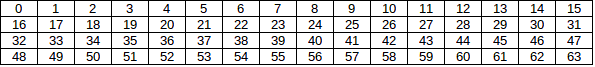
\includegraphics[scale=1]{figuras/fig101.png}
	\item Marque os múltiplos de 4.\\
	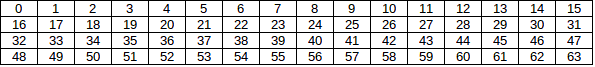
\includegraphics[scale=1]{figuras/fig101.png}
	\item Marque os múltiplos de 5.\\
	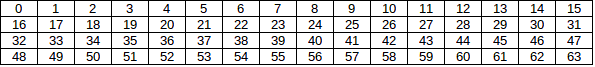
\includegraphics[scale=1]{figuras/fig101.png}
	\item Marque os múltiplos de 9.\\
	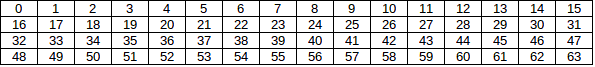
\includegraphics[scale=1]{figuras/fig101.png}
\end{enumerate}

\item Escreva certo ou errado.
\begin{enumerate}[a)]
\item O conjunto dos múltiplos de 7 é infinito.
\item O conjunto dos múltiplos de 5 é finito.
\item O conjunto dos múltiplos de 1 é unitário.
\item O menor múltiplo de qualquer número é zero.
\item O menor múltiplo de qualquer número é ele mesmo.
\item O conjunto  dos divisores de 12 é finito.
\item O conjunto dos divisores de 8 é infinito.
\item O conjunto dos divisores de 1 é unitário
\item O conjunto dos divisores de 7 é o vazio
\item O menor divisor de qualquer número é zero.
\item O menor divisor de qualquer número é 1.
\item O maior divisor de um número diferente de zero é ele mesmo.
\end{enumerate}

\item  Quais desses números são divisíveis por 2 ?
\begin{multicols}{5}
\begin{enumerate}[a)]
	\item 43
	\item 58
	\item 62
	\item 93
	\item 106
	\item 688
	\item 981
	\item 1000
	\item 3214
	\item 6847
	\item 14649
	\item 211116
	\item 240377
	\item 800001
	\item 647731350
\end{enumerate}
\end{multicols}

\item Quais desses números são divisíveis por 3?
\begin{multicols}{4}
\begin{enumerate}[a)]
	\item 72
	\item 83
	\item 58
	\item 96
	\item 123
	\item 431
	\item 583
	\item 609
	\item 1111
	\item 1375
	\item 1272
	\item 4932
	\item 251463
	\item 1040511
	\item 8000240
	\item 7112610
\end{enumerate}
\end{multicols}

\item Quais desses números são divisíveis por 4?
\begin{multicols}{4}
\begin{enumerate}[a)]
	\item 200
	\item 323
	\item 832
	\item 918
	\item 1020
	\item 3725
	\item 4636
	\item 7812
	\item 19012
	\item 24714
	\item 31433
	\item 58347
	\item 1520648
	\item 3408549
	\item 5331122
	\item 2000008
\end{enumerate}
\end{multicols}

\item Quais desses números são divisíveis por 5?
\begin{multicols}{4}
\begin{enumerate}[a)]
	\item 83
	\item 45
	\item 678
	\item 840
	\item 1720
	\item 1089
	\item 2643
	\item 4735
	\item 2643
	\item 8310
	\item 7642
	\item 12315
	\item 471185
	\item 648933
	\item 400040
	\item 3821665
\end{enumerate}
\end{multicols}

\item Quais destes números são divisíveis por 6?
\begin{multicols}{4}
\begin{enumerate}[a)]
	\item 126
	\item 452
	\item 831
	\item 942
	\item 1236
	\item 3450
	\item 2674
	\item 7116
	\item 10008
	\item 12144
	\item 12600 
	\item 51040
	\item 521125
	\item 110250
	\item 469101
	\item 4000002
\end{enumerate}
\end{multicols}

\item Quais desses números são divisíveis por 9?
\begin{multicols}{4}
\begin{enumerate}[a)]
	\item 504
	\item 720
	\item 428
	\item 818
	\item 3169
	\item 8856
	\item 4444
	\item 9108
	\item 29133
	\item 36199
	\item 72618
	\item 98793
	\item 591218
	\item 903402
	\item 174150
	\item 2000601
\end{enumerate}
\end{multicols}

\item Quais destes números são divisíveis por 10?
\begin{multicols}{4}
\begin{enumerate}[a)]
	\item 482
	\item 520
	\item 655
	\item 880
	\item 1670
	\item 1829
	\item 3687
	\item 8730
	\item 41110
	\item 29490
	\item 34002
	\item 78146
	\item 643280
	\item 128456
	\item 890005
	\item 492370
\end{enumerate}
\end{multicols}

\item determine:
\begin{multicols}{4}
\begin{enumerate}[a)]
	\item d(14);
	\item d(13);
	\item d(15);
	\item d(16).
\end{enumerate}
\end{multicols}

\item Efetue as divisões e responda:
\begin{multicols}{2}
\begin{enumerate}[a)]
	\item 495 é divisível por 9?
	\item 1260 é divisível por 7?
	\item 378 é divisível por 12?
	\item 14 é divisível por 182?
\end{enumerate}
\end{multicols}

\item Verifique se 182 é divisível por 7, por 8, por 11 e por 13.

\item Escreva:
\begin{multicols}{2}
\begin{enumerate}[a)]
	\item o número natural que só tem um divisor;
	\item um número natural que fica entre 20 e 30 e tem exatamente dois divisores;
	\item o número natural que tem infinitos divisores;
	\item um número natural que tem mais do que 8 divisores.
\end{enumerate}
\end{multicols}

\item Para descobrir os divisores de 8, há necessidade de dividir 8 por números naturais maiores do que ele? Responda e justifique.

\item Determine:
\begin{enumerate}[a)]
	\item os divisores comuns de 12 e 20, isto é, os números que são divisores de 12 e também são divisores de 20;
	\item os divisores comuns de 14 e 9.
\end{enumerate}

\item O mês de março possui 31 dias. Celso jogou tênis, neste  mês, nos dias ímpares e Rodrigo nos dias múltiplos de 3. Quantas vezes ambos jogaram tênis no mesmo dia? 

\item Quantos são os números primos até 30? Responda usando o crivo de Eratóstenes e a tabela abaixo.
\begin{center}
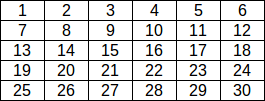
\includegraphics[scale=1]{figuras/fig102.png}
\end{center}

\item Quais são os números divisíveis por 6 entre 70 e 100 ?

\item Dados os números 39, 140, 245, 384, 720 e 2600, verifique os que são divisíveis por :
\begin{multicols}{2}
\begin{enumerate}[a)]
	\item 2
	\item 3
	\item 4
	\item 5
	\item 6
	\item 8
	\item 9
	\item 10
\end{enumerate}
\end{multicols}

\item Qual é o maior número de dois algarismos divisível por 5 ?

\item Qual é o menor número de três algarismos divisível por 3 ?

\item Um número é composto de três algarismos. O algarismo das unidades é 2 e o das centenas é 5. Determine os possíveis valores do algarismo das dezenas para que esse número seja divisível por 3.

\item Este é um jogo de números cruzados, parecido com as palavras cruzadas. Você deverá substituir os espaços por um algarismo, de modo que os números formados estejam de acordo com as seguintes instruções :

Horizontais :

A – Um número em que cada algarismo é o sucessor do algarismo anterior.\\
B – O maior número de três algarismos que seja divisível por 2.\\
C – Um número menor que 300.

Verticais :

A – Um número que não é divisível por 2.\\
B – Um número divisível por 3, mas não por 2.\\
C – Um número de três algarismos iguais.\\
\begin{center}
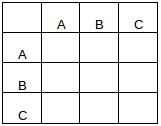
\includegraphics[scale=1]{figuras/fig103.png}
\end{center}
\end{list}
	\chapter{Problemas para o 7º ano.}
%==============================================================================================
\section{Expressões Numéricas}
\begin{list}{\textbf{Questão \arabic{quest}.}}{\usecounter{quest}}
%define a margem da lista.	
%\setlength{\labelwidth}{-2mm} \setlength{\parsep}{0mm}
%\setlength{\topsep}{0mm} \setlength{\leftmargin}{-2mm}
\renewcommand{\labelenumi}{(\alph{enumi})}

\item Calcule o valor das expressões
	\begin{multicols}{2}
	\begin{enumerate}[a)]
	\item $25-[10+(7-4)] =    (R:12)$
	\item $32+[10-(9-4)+8] =                         (R:45)$
	\item $45-[12-4+(2+1)] =                          (R:34)$
	\item $70-\{20-[10-(5-1)]\} =                     (R:56)$
	\item $28+\{13-[6-(4+1)+2]-1\} =              (R:37)$
	\item $53-\{20-[30-(15-1+6)+2]\} =           (R:45)$
	\item $62-\{16-[7-(6-4)+1]\} =                   (R:52)$
	\item $20-\{8+[3+(8-5)-1]+6\} =                (R:1)$
	\item $15+\{25-[2-(8-6)]+2\} =                   (R:42)$
	\item $56-[3+(8-2)+(51-10)-(7-2)] =          (R:11)$
	\end{enumerate}
	\end{multicols}

\item Calcule as expressões
	\begin{multicols}{2}
	\begin{enumerate}[a)]
		\item $3\cdot75+3\cdot25= (R:300)$
		\item $5\cdot97+5\cdot3= (R:500 )$
		\item $4\cdot101+4\cdot99= (R:800)$
		\item $20\cdot47+80\cdot47= (R:4700)$
		\item $12+16:8\cdot3-5= (R:13)$
		\item $100-6\cdot7+8:2 = (R:62)$
		\item $64:8+5\cdot5-3= (R: 30)$
		\item $1+3+5\cdot7-9:3 = (R:36)$
	\end{enumerate}
	\end{multicols}

\item Calcule o valor das expressões:
	\begin{multicols}{2}
	\begin{enumerate}[a)]
		\item $7+15:3                    = (R:12)$
		\item $4\cdot5+1                     = (R:21)$
		\item $10:2+8                    = (R:13)$
		\item $32+12:2                  = (R:38)$
		\item $20:10+10                = (R:12)$
		\item $7\cdot3-2\cdot5                   = (R:11)$
		\item $40-2\cdot4+5                 = (R:37)$
		\item $4\cdot3+10:2                 = (R:17)$
		\item $50-16:8+7                 = (R:55)$
		\item $32:4:2:2                    = (R:2)$
	\end{enumerate}
	\end{multicols}

\item Calcule o valor das expressões
	\begin{multicols}{2}
	\begin{enumerate}[a)]
		\item $(13+2)\cdot3+5            = (R:50)$
		\item $(7+2\cdot(3-1)              = (R:18)$
		\item $(4+2\cdot5)-3                = (R:11)$
		\item $20-(15+6:3)                        = (R:3)$
		\item $15+[6+(8-4:2)]                    = (R:27)$
		\item $40-[3+(10-2):2]                    = (R:33)$
		\item $[30+2\cdot(5-3)]\cdot2-10              = (R:58)$
		\item $10+[4+(7\cdot3+1)]-3              = (R:33)$
	\end{enumerate}
	\end{multicols}


\item Calcule o valor das expressões
	\begin{multicols}{2}
	\begin{enumerate}[a)]
		\item $(3+2)\cdot(5-1)+4                    = (R:24)$
		\item $82-8\cdot7:(4-1\cdot3)                   = (R:26)$
		\item $25-[10-(2\cdot3+1)]                 = (R:22)$
		\item $70-[12+(5\cdot2-1)+6]             = (R:43)$
		\item $8:2+[15-(4\cdot2+1)]                = (R:10)$
		\item $9+[4+2\cdot(6-4)+(2+5)]-8                   = (R:16)$
		\item $50+\{10-2\cdot[(6+4:2)-(10-3)]\}                      = (R:58)$
		\item $180:\{10+2\cdot[20-45:(13-2\cdot5)]\}                    = (R:9)$
	\end{enumerate}
	\end{multicols}



\item Calcule o valor das expressões:
	\begin{multicols}{2}
	\begin{enumerate}[a)]
		\item $70:7-1                     = (R:9)$
		\item $20+3\cdot2= (R:26)$
		\item $30+10:10                = (R:31)$
		\item $150-7\cdot12                = (R:66)$
		\item $48:16+20:4             = (R:8)$
		\item $10-8:2+3                 = (R:9)$
		\item $30:5-1+2\cdot3             = (R:11)$
	\end{enumerate}
	\end{multicols}


\item Calcule as expressões:
	\begin{multicols}{2}
	\begin{enumerate}[a)]
		\item $(3+4)\cdot(9-8)                         = (R:7)$
		\item $(20+8):(3+4)                      = (R:4)$
		\item $15+8\cdot(2+3)                        = (R:55)$
		\item $(5+3\cdot2)-1                           = (R:10)$
		\item $25+(8:2+1)-1                      = (R:29)$
		\item $15+[5\cdot(8-6:2)]                    = (R:40)$
		\item $50-[13-(10-2):2]                 = (R:41)$
		\item $[40+2\cdot(7-5)]\cdot2-20             = (R:68)$
	\end{enumerate}
	\end{multicols}

\item Calcule o valor das expressões:
	\begin{multicols}{2}
	\begin{enumerate}[a)]
		\item $16+[10-(18:3+2)+5]                       = (R: 23)$
		\item $25-[12-(3\cdot2+1)]                             = (R: 20)$
		\item $90-[25+(5\cdot2-1)+3]                         = ( R: 53)$
		\item $45+[(8\cdot5-10:2)+(18:6-2)]              = (R: 81)$
		\item $50-2\cdot\{7+8:2-[9-3\cdot(5-4)]\}              = (R: 40)$
		\item $100-3\cdot\{5+8:2-[3\cdot(7-6)]\}               = (R: 82)$
	\end{enumerate}
	\end{multicols}


\item Determine o valor de cada expressão
	\begin{multicols}{2}
	\begin{enumerate}[a)]
		\item $1000 - [(2 \cdot 4 - 6) + ( 2 + 6 \cdot 4)]      = (R: 972)$
		\item $60 + 2 \cdot \{[ 4 \cdot ( 6 + 2 ) - 10 ] + 12\}      = ( R: 128 )$
		\item $[( 4 + 16 \cdot 2) \cdot 5 - 10] \cdot 100   = (R: 17.000)$
		\item $\{ 10 + [ 5 \cdot ( 4 + 2 \cdot 5) - 8] \cdot 2 \} - 100  = ( R: 34)$
		\item $80 - 5 \cdot ( 28 - 6 \cdot 4 ) + 6 - 3 \cdot 4      = (R: 54)$
	\end{enumerate}
	\end{multicols}


\item Calcule
	\begin{multicols}{2}
	\begin{enumerate}[a)]
		\item $4 \cdot ( 10 + 20 + 15 + 30)  = (R: 300)$
		\item $(10 \cdot 6 + 12 \cdot 4 + 5 \cdot 8 ) - 40   = (R: 108)$
		\item $[ 6 \cdot ( 3 \cdot 4 - 2 \cdot 5) - 4 ] + 3 \cdot ( 4 - 2) - ( 10 : 2 ) = (R: 9)$
		\item $67 + \{ 50 \cdot [ 70 : ( 27 + 8 ) + 18 : 2 ] + 21 \}  = (R:638)$
		\item $[ 30 \cdot ( 9 - 6)] + [ 30 : ( 9 + 6 ) ]  = (R: 92)$
		\item $58 - [ 20 - ( 3 \cdot 4 - 2) : 5 ]= (R: 40)$
		\item $40 + 2 \cdot [ 20 - ( 6 + 4 \cdot 7 ) : 2 ] = ( R: 46)$
	\end{enumerate}
	\end{multicols}
\end{list}

%==============================================================================================
%=============================================================================================
\section{Geometria Espacial}

\begin{list}{\textbf{Questão \arabic{quest}.}}{\usecounter{quest}}
%define a margem da lista.	
%\setlength{\labelwidth}{-2mm} \setlength{\parsep}{0mm}
%\setlength{\topsep}{0mm} \setlength{\leftmargin}{-2mm}
\renewcommand{\labelenumi}{(\alph{enumi})}

\item  Observe a caixa representada abaixo:
\begin{center}
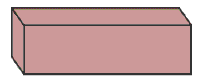
\includegraphics[scale=1]{figuras/fig80.png}
\end{center}
Uma planificação dessa caixa é:
\begin{multicols}{4}
\begin{enumerate}[a)]
	\item 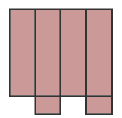
\includegraphics[scale=0.7]{figuras/fig80_a.png}
	\item 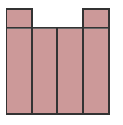
\includegraphics[scale=0.7]{figuras/fig80_b.png}
	\item 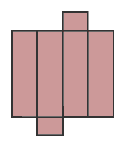
\includegraphics[scale=0.7]{figuras/fig80_c.png}
	\item 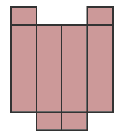
\includegraphics[scale=0.7]{figuras/fig80_d.png} 
\end{enumerate}
\end{multicols}

\item A forma geométrica espacial que pode ser associada à planificação abaixo é:
\begin{multicols}{2}
	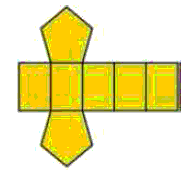
\includegraphics[scale=0.7]{figuras/fig81.png}
	\begin{enumerate}[a)]
		\item um cilindro
		\item uma pirâmide de base pentagonal 
		\item um prisma de base pentagonal.
		\item um paralelepípedo	
	\end{enumerate}
\end{multicols}

\item As figuras 1, 2 e 3 correspondem, respectivamente, às planificações dos sólidos:
\begin{center}
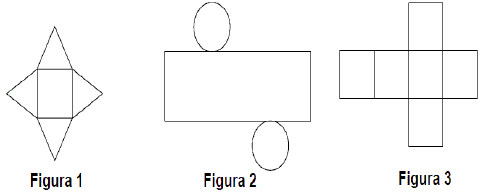
\includegraphics[scale=0.6]{figuras/fig82.png}
\end{center}
\begin{multicols}{4}
\begin{enumerate}[a)]
	\item Cubo, cone, pirâmide.
	\item Pirâmide, cilindro, cubo.
	\item Cubo, cilindro, pirâmide.
	\item Pirâmide, cone, cubo.
\end{enumerate}
\end{multicols}
\item Analise estes desenhos de poliedros e determine em cada um deles o número de vértices(V), o número de faces (F) e o número de arestas (A).
\begin{center}
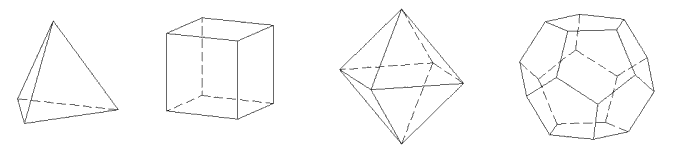
\includegraphics[scale=0.9]{figuras/fig83.png}
\end{center}

\end{list}

%==============================================================================================
%=============================================================================================
\section{Geometria Plana}

\begin{list}{\textbf{Questão \arabic{quest}.}}{\usecounter{quest}}
%define a margem da lista.	
%\setlength{\labelwidth}{-2mm} \setlength{\parsep}{0mm}
%\setlength{\topsep}{0mm} \setlength{\leftmargin}{-2mm}
\renewcommand{\labelenumi}{(\alph{enumi})}

\item Desenhe um polígono convexo e outro não convexo.
\item Calcule o número de diagonais em:
\begin{multicols}{2}
\begin{enumerate}[a)]
\item um polígono convexo de 11 lados;
\item um decágono(dez lados) convexo;
\item um icoságono(vinte lados) convexo;
\item um polígono convexo de 13 lados.
\end{enumerate}
\end{multicols}

\end{list}

%==============================================================================================
%=============================================================================================
\section{Números racionais}
\subsection{Atividades Introdutórias}
\begin{list}{\textbf{Questão \arabic{quest}.}}{\usecounter{quest}}
%define a margem da lista.	
%\setlength{\labelwidth}{-2mm} \setlength{\parsep}{0mm}
%\setlength{\topsep}{0mm} \setlength{\leftmargin}{-2mm}
\renewcommand{\labelenumi}{(\alph{enumi})}


\item Simplifique as frações.
\begin{multicols}{6}
\begin{enumerate}[a)]
	\item $\dfrac{10}{20}$
	\item $\dfrac{15}{35}$
	\item $\dfrac{6}{2}$
	\item $\dfrac{50}{60}$
	\item $\dfrac{20}{100}$
	\item $\dfrac{35}{40}$
	\item $\dfrac{16}{24}$
	\item $\dfrac{12}{16}$
	\item $\dfrac{20}{90}$
	\item $\dfrac{49}{63}$
	\item $\dfrac{12}{21}$
	\item $\dfrac{13}{15}$
	\item $\dfrac{19}{25}$
	\item $\dfrac{45}{82}$
	\item $\dfrac{50}{10}$
	\item $\dfrac{54}{27}$
	\item $\dfrac{9}{72}$
	\item $\dfrac{6}{17}$
	\item $\dfrac{65}{70}$
	\item $\dfrac{2}{3}$
	\item $\dfrac{7}{42}$
	\item $\dfrac{11}{120}$
	\item $\dfrac{56}{64}$
	\item $\dfrac{85}{24}$			
\end{enumerate}
\end{multicols}

\item Para cada item, escreva duas frações equivalentes.
\begin{multicols}{6}
\begin{enumerate}[a)]
	\item $\dfrac{1}{2}$		
	\item $\dfrac{2}{5}$		
	\item $\dfrac{7}{2}$		
	\item $\dfrac{8}{9}$		
	\item $\dfrac{5}{7}$		
	\item $\dfrac{9}{13}$		
	
	\item $\dfrac{2}{7}$		
	\item $\dfrac{11}{2}$		
	\item $\dfrac{7}{10}$		
	\item $\dfrac{9}{17}$		
	\item $\dfrac{1}{9}$		
	\item $\dfrac{8}{5}$		

	\item $\dfrac{10}{11}$		
	\item $\dfrac{7}{4}$		
	\item $\dfrac{4}{7}$		
	\item $\dfrac{2}{3}$		
	\item $\dfrac{6}{2}$		
	\item $\dfrac{20}{21}$		

	\item $\dfrac{21}{35}$		
	\item $\dfrac{1}{100}$		
	\item $\dfrac{1}{1000}$		
	\item $\dfrac{4}{50}$		
	\item $\dfrac{9}{40}$		
	\item $\dfrac{10}{100}$		
\end{enumerate}
\end{multicols}

\item Calcule:
\begin{multicols}{4}
\begin{enumerate}[a)]
	\item $mmc(2,4)=$
	\item $mmc(4,5)=$
	\item $mmc(6,7)=$
	\item $mmc(3,4)=$
	\item $mmc(8,12)=$

	\item $mmc(6 ,4 )=$
	\item $mmc(4,6)=$
	\item $mmc(10,100 )=$
	\item $mmc(6,18)=$
	\item $mmc(12,24)=$

	\item $mmc(13,9)=$
	\item $mmc(6,7)=$
	\item $mmc(9,10)=$
	\item $mmc(3,5)=$
	\item $mmc(6,11)=$

	\item $mmc(2,3,5)=$
	\item $mmc(3,4,5)=$
	\item $mmc(3,6,12)=$
	\item $mmc(5,10,20)=$
	\item $mmc(3,4,17)=$

\end{enumerate}
\end{multicols}

\item Reduza ao menor denominador comum as seguintes frações:
\begin{multicols}{3}
\begin{enumerate}[a)]
	\item $\dfrac{9}{4}\ , \dfrac{6}{7}$
	\item $\dfrac{7}{9}\ ,\ \dfrac{5}{3}$
	\item $\dfrac{3}{10}\ ,\ \dfrac{7}{15}$

	\item $\dfrac{1}{8}\ ,\ \dfrac{1}{5},\ \dfrac{1}{10}$
	\item $\dfrac{3}{4}\ ,\ \dfrac{7}{6},\ \dfrac{8}{9}$
	\item $\dfrac{5}{12}\ ,\ \dfrac{3}{8},\ \dfrac{1}{6}$
\end{enumerate}
\end{multicols}

\item Escreva em forma de fração imprópria:
\begin{multicols}{6}
\begin{enumerate}[a)]
	\item $4\frac{1}{2}$
	\item $7\frac{2}{3}$
	\item $5\frac{3}{4}$
	\item $1\frac{4}{7}$
	\item $10\frac{1}{2}$
	\item $11\frac{1}{5}$
\end{enumerate}
\end{multicols}

\item Escreva em forma de mista as seguintes frações impróprias:
\begin{multicols}{6}
\begin{enumerate}[a)]
	\item $\dfrac{16}{5}$
	\item $\dfrac{17}{3}$
	\item $\dfrac{31}{3}$
	\item $\dfrac{9}{2}$
	\item $\dfrac{11}{7}$
	\item $\dfrac{20}{6}$
\end{enumerate}
\end{multicols}

\item Calcule:
\begin{multicols}{3}
\begin{enumerate}[a)]
	\item $2\frac{1}{5} + \dfrac{3}{4}$
	\item $1\frac{1}{6} + 1\frac{1}{9}$
	\item $\dfrac{7}{10} + 2\frac{3}{4}$
\end{enumerate}
\end{multicols}

\item Calcule e simplifique, quando for possível, o resultado:
\begin{multicols}{3}
\begin{enumerate}[a)]
	\item $\dfrac{5}{7} - \dfrac{2}{7} = $
	\item $\dfrac{7}{8} - \dfrac{3}{8} = $
	\item $\dfrac{2}{9} - \dfrac{2}{9} = $

	\item $\dfrac{6}{6} - \dfrac{1}{6} = $
	\item $\dfrac{9}{10} - \dfrac{1}{10} = $
	\item $\dfrac{7}{12} - \dfrac{5}{12} = $

	\item $\dfrac{7}{5} - \dfrac{3}{5} + \dfrac{2}{5} = $
	\item $\dfrac{7}{9} + \dfrac{3}{9} - \dfrac{4}{9} = $
	\item $\dfrac{8}{8} - \dfrac{7}{8} + \dfrac{1}{8} = $
\end{enumerate}
\end{multicols}

\item Qual alternativa representa a fração 9/2 em números decimais?
\begin{multicols}{4}
\begin{enumerate}[a)]
	\item 3,333
	\item 4,25
	\item 5,01
	\item 4,5
\end{enumerate}
\end{multicols}

\item Qual alternativa representa a fração 35/1000 em números decimais?
\begin{multicols}{4}
\begin{enumerate}[a)]
	\item 0,35
	\item 3,5
	\item 0,035
	\item 35
\end{enumerate}
\end{multicols}

\item Qual é a alternativa que representa o número 0,65 na forma de fração?
\begin{multicols}{4}
\begin{enumerate}[a)]
	\item $\displaystyle\frac{65}{10}$
	\item $\displaystyle\frac{65}{100}$
	\item $\displaystyle\frac{65}{1000}$
	\item $\displaystyle\frac{65}{10000}$
\end{enumerate}
\end{multicols}

\item Observe as frações e suas respectivas representações decimais.
\begin{multicols}{4}
\begin{enumerate}[a)]
	\item $\displaystyle\frac{3}{1000}=0,003$
	\item $\displaystyle\frac{2367}{100}=23,67$
	\item $\displaystyle\frac{129}{1000}-0,129$
	\item $\displaystyle\frac{65}{10000}=0,065$
\end{enumerate}
\end{multicols}

Utilizando as igualdades acima, escolha a alternativa correta?
\begin{multicols}{4}
\begin{enumerate}[a)]
	\item I e II
	\item I e IV
	\item I, II e III
	\item I, II, III e IV
\end{enumerate}
\end{multicols}

\item Qual alternativa representa a soma dos números decimais 0,65 e 0,15?
\begin{multicols}{4}
\begin{enumerate}[a)]
	\item 0,80
	\item 0,77
	\item 0,67
	\item 1,00
\end{enumerate}
\end{multicols}

\item Qual alternativa representa a soma $S=4,013+10,182$?
\begin{multicols}{4}
\begin{enumerate}[a)]
	\item 14,313
	\item 13,920
	\item 14,195
	\item 14,083
\end{enumerate}
\end{multicols}

\item Qual é a diferença entre os números decimais 724,96 e 242,12?
\begin{multicols}{4}
\begin{enumerate}[a)]
	\item 48,284
	\item 586,28
	\item 241,59
	\item 482,84
\end{enumerate}
\end{multicols}

\item Qual é a alternativa que representa a subtração 3,02-0,65?
\begin{multicols}{4}
\begin{enumerate}[a)]
	\item 2,37
	\item 3,37
	\item 1,32
	\item 23,7
\end{enumerate}
\end{multicols}

\item Para cada caso, somar os números.
\begin{multicols}{4}
\begin{enumerate}[a)]
	\item 0,25 + 1,25
	\item 0,25 + 2,5
	\item 0,25 + 3,7
	\item 0,25 + 6,2
	\item 0,3 + 1,25
	\item 0,3 + 2,5
	\item 0,3 + 3,7
	\item 0,3 + 6,2
\end{enumerate}
\end{multicols}

\item Para cada caso, subtrair os números.
\begin{multicols}{4}
\begin{enumerate}[a)]
	\item 0,25 - 1,25
	\item 0,25 - 2,5
	\item 0,25 - 3,7
	\item 0,25 - 6,2
	\item 0,3 - 1,25
	\item 0,3 - 2,5
	\item 0,3 - 3,7
	\item 0,3 - 6,2
\end{enumerate}
\end{multicols}

\item O número decimal 0,03 pode ser escrito por extenso como:
\begin{multicols}{4}
\begin{enumerate}[a)]
	\item três décimos
	\item três centésimos
	\item três milésimos
\end{enumerate}
\end{multicols}

\item Associar o número 15,435 à alternativa que o representa:
\begin{enumerate}[a)]
	\item Quinze inteiros e quatrocentos e trinta e cinco centésimos
	\item Cento e cinquenta e quatro e trinta e cinco centésimos
	\item Quinze inteiros e quatrocentos e trinta e cinco milésimos
\end{enumerate}

\item Assinalar a alternativa com a resposta da adição $4/7+2/7$:
\begin{multicols}{4}
\begin{enumerate}[a)]
	\item $\displaystyle\frac{5}{7}$
	\item $\displaystyle\frac{6}{14}$
	\item $\displaystyle\frac{7}{6}$
	\item $\displaystyle\frac{6}{7}$	
\end{enumerate}
\end{multicols}

\item Qual das alternativas representa a subtração $8/9-6/9$?
\begin{multicols}{4}
\begin{enumerate}[a)]
	\item $-\displaystyle\frac{2}{9}$
	\item $\displaystyle\frac{2}{9}$
	\item $\displaystyle\frac{14}{9}$
	\item $\displaystyle\frac{1}{4}$	
\end{enumerate}
\end{multicols}

\item Qual alternativa representa a dízima periódica $0,555...$ ?
\begin{multicols}{4}
\begin{enumerate}[a)]
	\item $-\displaystyle\frac{5}{3}$
	\item $\displaystyle\frac{5}{2}$
	\item $\displaystyle\frac{5}{4}$
	\item $\displaystyle\frac{5}{9}$	
\end{enumerate}
\end{multicols}

\item Qual é a fração mais simples que equivale a $14/21$?

\item A área colorida em cada círculo indica uma fração de um inteiro. Qual alternativa representa a soma destas frações?
\begin{center}
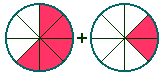
\includegraphics[scale=1]{figuras/fig99.png}
\end{center}
\begin{multicols}{4}
\begin{enumerate}[a)]
	\item $\displaystyle\frac{5}{8}$
	\item $\displaystyle\frac{7}{8}$
	\item $\displaystyle\frac{9}{8}$
	\item $\displaystyle\frac{8}{7}$
\end{enumerate}
\end{multicols}
\end{list}

%==============================================================================================
\subsection{Adição e Subtração de Números Racionais}
\begin{list}{\textbf{Questão \arabic{quest}.}}{\usecounter{quest}}
%define a margem da lista.	
%\setlength{\labelwidth}{-2mm} \setlength{\parsep}{0mm}
%\setlength{\topsep}{0mm} \setlength{\leftmargin}{-2mm}
\renewcommand{\labelenumi}{(\alph{enumi})}

\item Efetue as adições e subtrações.
\begin{multicols}{3}
\begin{enumerate}[a)]
	\item $\displaystyle\left(-\frac{2}{3}\right)+\left(+\frac{1}{4}\right)$
	\item $\displaystyle\left(-\frac{4}{7}\right)+\left(-\frac{2}{6}\right)$
	\item $\displaystyle\left(+\frac{1}{7}\right)-\left(+\frac{1}{3}\right)$
	\item $\displaystyle\left(+\frac{2}{3}\right)-\left(+\frac{1}{3}\right)$
	\item $\displaystyle\left(-\frac{4}{5}\right)-\left(-\frac{1}{8}\right)$
	\item $\displaystyle\left(-\frac{3}{4}\right)- 5$
\end{enumerate}
\end{multicols}

\item Calcule.
\begin{multicols}{2}
\begin{enumerate}[a)]
	\item $(+3,8)+(+5,72)$
	\item $(-1,75)+(+3,84)$
	\item $(+5,5)-(+8,13)$
	\item $(-4,72)-(-0,28)$
\end{enumerate}
\end{multicols}

\item Calcule o valor de cada expressão:
\begin{multicols}{3}
\begin{enumerate}[a)]
	\item $\displaystyle\frac{3}{7}-1+\frac{4}{3}$
	\item $\displaystyle\frac{7}{8}-\frac{1}{4}+\frac{2}{3}$
	\item $-0,25+1,5-0,3$
	\item $-\displaystyle\frac{5}{12}-\frac{1}{12}+\frac{4}{6}$
	\item $0,375-0,125 - 0,625$
	\item $\displaystyle\frac{1}{5}-2+\frac{1}{7}$
\end{enumerate}
\end{multicols}

\item Qual é o valor de cada expressão?
\begin{multicols}{2}
\begin{enumerate}[a)]
	\item $1,7+\left(\displaystyle\frac{2}{3}-0,25\right) - \displaystyle\frac{1}{4}$
	\item $\left[1,6+\left(\displaystyle\frac{1}{4}-0,75+2 \right)-\displaystyle\frac{3}{5}\right]$
\end{enumerate}
\end{multicols}

\item Um submarino encontra-se a $-60$ m de profundidade, se descer o dobro, que profundidade o submarino atingirá?

\item Em certo mês, uma cidade do Sul do país teve sua temperatura máxima de 14,5 ºC e temperatura mínima de $-2,8$ ºC. Qual foi a diferença entre as temperaturas máxima e mínima registradas nesse mês?

\item Lina possuía R\$ 312,50. Recebeu R\$ 250,00 do seu pai e efetuou 3 pagamentos nos valores de R\$ 108,15, R\$ 89,00 e R\$ 204,50. Com quanto Lina ficou?

\item Vitor gastou, em maio, $\frac{1}{3}$ do seu salário com alimentação e $\frac{1}{2}$ com entretenimento, sobrando-lhe ainda R\$ 315,00. Qual foi o salário de Vítor nesse mês?

\item Calcule as somas:
\begin{multicols}{2}
\begin{enumerate}[a)]
	\item $\displaystyle\frac{2}{5}+\left(-\frac{1}{3}\right)$
	\item $\displaystyle\left(-\frac{2}{3}\right)+\left(-\frac{5}{6}\right)$
	\item $\displaystyle\frac{3}{5}+ \left(-\frac{1}{3}\right)+\left(-\frac{2}{5}\right)$
	\item $(+0,1)+(-1,1)+(+0,11)$
\end{enumerate}
\end{multicols}

\item Efetue as subtrações:
\begin{multicols}{2}
\begin{enumerate}[a)]
	\item $\displaystyle\frac{2}{5}-\left(+\frac{1}{4}\right)$
	\item $\displaystyle\left(-\frac{5}{8}\right)-\left(+\frac{3}{8}\right)$
	\item $\displaystyle\left(+\frac{1}{4}\right)-\left(-\frac{1}{2}\right)$
	\item $(-0,54)-(-0,6)$
	\item $-\displaystyle\frac{1}{4}-\left(-\frac{1}{8}\right)$
	\item $\displaystyle\left(-\frac{4}{5}\right)-(+3,8)$
\end{enumerate}
\end{multicols}

\item Calcule o valor das expressões:
\begin{enumerate}[a)]
	\item $\displaystyle\left(+\frac{7}{6}\right)+\left(-\frac{5}{6}\right)$
	\item $\displaystyle\left(+\frac{1}{2}\right)-\left(-\frac{5}{2}\right)+\left(-\frac{3}{2}\right)$
	\item $-\displaystyle\frac{1}{4}+\left(+\frac{3}{5}\right)+\left(-\frac{1}{10}\right)$
	\item $\displaystyle\frac{1}{5}-\left[\frac{2}{3}-\left(\frac{2}{6}-\frac{1}{12}\right)\right]+\frac{5}{6}$
	\item $\left[\left(-\displaystyle\frac{1}{6}\right)+\left(\displaystyle\frac{1}{2}-\frac{1}{3}\right)\right]-\left[\displaystyle\frac{2}{3}+\left(-\frac{1}{2}-\frac{5}{6}\right)\right]$
	\item $[0,4-(0,62-1,8)+(-1,5+1,2)]-0,6$
\end{enumerate}

\item Dê exemplos de dos números racionais cuja soma seja:
\begin{multicols}{4}
\begin{enumerate}[a)]
	\item $-\displaystyle\frac{4}{5}$
	\item $0,7$
	\item $+\displaystyle\frac{1}{2}$
	\item $-6,3$
\end{enumerate}
\end{multicols}

\begin{multicols}{2} 
\item  Determine os números A,B e C da figura, sabendo que a soma dos números situados em qualquer lado é sempre 15.
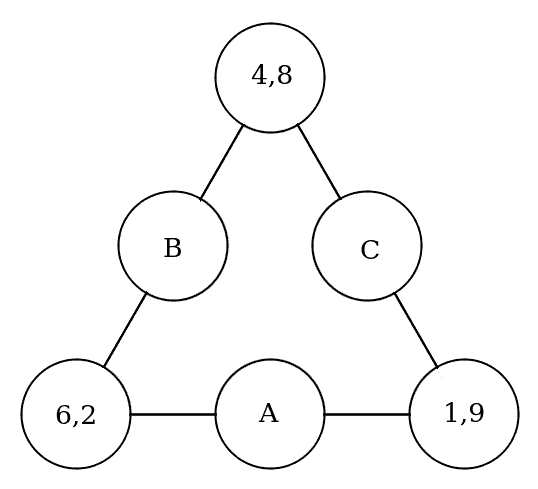
\includegraphics[scale=0.3]{figuras/fig100.png}
\end{multicols}
\end{list}

%==============================================================================================
\subsection{Multiplicação de Números Racionais}
\begin{list}{\textbf{Questão \arabic{quest}.}}{\usecounter{quest}}
%define a margem da lista.	
%\setlength{\labelwidth}{-2mm} \setlength{\parsep}{0mm}
%\setlength{\topsep}{0mm} \setlength{\leftmargin}{-2mm}
\renewcommand{\labelenumi}{(\alph{enumi})}

\item Determine os produtos:
\begin{multicols}{4}
\begin{enumerate}[a)]
	\item $\displaystyle\left(+\frac{2}{3}\right)\cdot\left(-\frac{2}{5}\right)$
	\item $\displaystyle\left(-\frac{3}{4}\right)\cdot\left(-\frac{2}{7}\right)$
	\item $\displaystyle\left(-\frac{3}{5}\right)\cdot\left(+\frac{5}{6}\right)$
	\item $(-0,5)\cdot (-2,0)$
\end{enumerate}
\end{multicols}

\item Determine o valor de cada expressão:
\begin{multicols}{2}
\begin{enumerate}[a)]
	\item $(+2)\cdot \displaystyle\left(-\frac{3}{4}\right)\cdot \left(+\frac{1}{6}\right)$
	\item $\displaystyle\left[\left(-\frac{1}{5}+\frac{3}{4}+1\right)\cdot \left(-\frac{1}{3}\right)\right]$
\end{enumerate}
\end{multicols}

\item Calcule o valor de cada expressão:
\begin{multicols}{2}
\begin{enumerate}[a)]
	\item $(-0,15)\cdot (+0,1)-(+0,6)\cdot (-0,21)$
	\item $(-3)\cdot (-1,6) - (+2)\cdot (-1,3)$
\end{enumerate}
\end{multicols}

\item Calcule o valor das expressões:
\begin{multicols}{3}
\begin{enumerate}[a)]
	\item $(5,4)\cdot (-3,2)$
	\item $(-1,08)\cdot (-2,5)$
	\item $(-3,85)\cdot (+2,4))$
	\item $(+1,4)\cdot (-0,5)$
	\item $(+10,6)\cdot (+8,17)$
	\item $(-8,35)\cdot (-1,17)$
\end{enumerate}
\end{multicols}

\item Efetue as multiplicações.
\begin{multicols}{2}
\begin{enumerate}[a)]
	\item $\left(-\displaystyle\frac{4}{5}\right)\cdot \left(-\displaystyle\frac{7}{4}\right)$
	\item $\left(+\displaystyle\frac{4}{9}\right)\cdot \left(-\displaystyle\frac{16}{81}\right)$
	\item $\displaystyle\left(+\frac{5}{8}\right)\cdot\left(-\frac{4}{3}\right)$
	\item $\left(+\displaystyle\frac{4}{5}\right)\cdot 0$
	\item $(+3)\cdot\displaystyle\left(-\frac{3}{9}\right)\cdot\left(+\frac{18}{6}\right)$
\end{enumerate}
\end{multicols}

\item Isadora vai revestir uma das paredes de seu quarto com um papel decorativo. Essa parede tem 4,35 m de comprimento por 2,80 m de largura. Quantos metros quadrados de papel decorativo serão necessários para cobrir essa parede?

\item Determine o produto dos números $-14$ e $-0,025$.

\item Calcule o valor da expressão: $\left(-\displaystyle\frac{3}{4}\cdot\frac{16}{81} +0,3\right)\cdot \left(-\displaystyle\frac{3}{4}\right)$

\item Em uma sessão de cinema foram vendidos 328 ingressos, sendo 80 meias-entradas. Calcule o valor arrecadado nessa sessão. Sabendo que o preço do ingresso (inteiro) custa R\$ 16,50.

\item Pedro comprou uma moto. Ele pagou $\displaystyle\frac{3}{10}$ de entrada e dividiu o restante em 20 parcelas iguais de R\$ 217,70. Qual foi o valor da moto?
\end{list}

%==============================================================================================
\subsection{Divisão de Números Racionais}
\begin{list}{\textbf{Questão \arabic{quest}.}}{\usecounter{quest}}
%define a margem da lista.	
%\setlength{\labelwidth}{-2mm} \setlength{\parsep}{0mm}
%\setlength{\topsep}{0mm} \setlength{\leftmargin}{-2mm}
\renewcommand{\labelenumi}{(\alph{enumi})}


\item Calcule o valor das divisões.
\begin{multicols}{2}
\begin{enumerate}[a)]
	\item $\left(+\dfrac{1}{4}\right): \left(-\dfrac{1}{2}\right)$
	\item $\left(-\dfrac{2}{5}\right): (+3)$
	\item $\left(-\dfrac{3}{25}\right): \left(-\dfrac{9}{10}\right)$
	\item $(-5):(-10)$
	\item $(-2,5):\left(+\dfrac{2}{100}\right)$
	\item $5:\left(-\dfrac{3}{4}\right)$
\end{enumerate}
\end{multicols}

\item Calcule o valor das expressões.
\begin{enumerate}[a)]
	\item $\left(-\dfrac{3}{4}\right) + \left(-\dfrac{1}{2}\right):\left(+\dfrac{1}{4}\right)$
	\item $\left[(+2) - \left(-\dfrac{3}{2}\right):\left(-\dfrac{3}{2}\right)\right]\cdot\left(-\dfrac{1}{2}\right)$
	\item $\left[\left(+\dfrac{1}{2}\right)\cdot \left(-\dfrac{3}{4}\right) - \left(+\dfrac{1}{2}\right) : \left(-\dfrac{2}{3}\right)\right]: \left(-\dfrac{3}{4}\right)$
	\item $(-3)\cdot (+1,25) - (+1,2) : (0,6)$
\end{enumerate}

\item Determine o valor de:
\begin{multicols}{2}
\begin{enumerate}[a)]
	\item $\dfrac{\left(-\dfrac{2}{5}\right)}{\left(-\dfrac{8}{10}\right)}$
	\item $\dfrac{\left(-\dfrac{1}{2}\right) + \left(+\dfrac{2}{3}\right)}{\left( -\dfrac{1}{6} \right) - \left(-\dfrac{1}{3} \right)}$
	\item $1 + \dfrac{\left(-\dfrac{1}{2}\right)}{\left(-\dfrac{2}{3}\right)}$
	\item $\dfrac{\left(-\dfrac{3}{4}\right)\cdot \left(-\dfrac{2}{5}\right)}{\left(\dfrac{1}{6} \right)}$
\end{enumerate}
\end{multicols}

\item Calcule o valor das expressões.
\begin{multicols}{2}
\begin{enumerate}[a)]
	\item $-27,6:1,5$
	\item $(-4,9):(-0,98)$
\end{enumerate}
\end{multicols}

\item Calcule o valor das expressões.
\begin{multicols}{2}
\begin{enumerate}[a)]
	\item $(-200):(+0,5)$
	\item $(+16,2):(-3,6)$
	\item $(-81,64):(-6,5)$
	\item $(+12,6):(-0,25)$
\end{enumerate}
\end{multicols}

\item Efetue as divisões.
\begin{multicols}{2}
\begin{enumerate}[a)]
	\item $\left(+\displaystyle\frac{7}{6}\right):\left(-\displaystyle\frac{1}{7}\right)$
	\item $\left(-\displaystyle\frac{4}{7}\right):\left(-\displaystyle\frac{8}{7}\right)$
	\item $\left(+\displaystyle\frac{3}{7}\right):\left(+\displaystyle\frac{21}{49}\right)$
	\item $\left(-\displaystyle\frac{3}{5}\right):\left(-\displaystyle\frac{9}{15}\right)$
	\item $\left(-\displaystyle\frac{4}{9}\right):\left(+\displaystyle\frac{16}{81}\right)$
	\item $\left(-\displaystyle\frac{5}{2}\right):(+8)$
	\item $(+16):\left(-\displaystyle\frac{3}{8}\right)$
	\item $\left(-\displaystyle\frac{3}{5}\right):(+0,1)$
\end{enumerate}
\end{multicols}

\item Jorge tinha um terreno de 23 575 metros quadrados. Ele reservou 6 100 metros quadrados desse terreno para área de lazer. Do que restou, Jorge reservou $\displaystyle\frac{1}{5}$ para estacionamento e dividiu o restante em lotes de 349,50 metros quadrados cada um. Quantos lotes Jorge obteve?
\end{list}

%==============================================================================================
\subsection{Potenciação de Números Racionais}
\begin{list}{\textbf{Questão \arabic{quest}.}}{\usecounter{quest}}
%define a margem da lista.	
%\setlength{\labelwidth}{-2mm} \setlength{\parsep}{0mm}
%\setlength{\topsep}{0mm} \setlength{\leftmargin}{-2mm}
\renewcommand{\labelenumi}{(\alph{enumi})}


\item Efetue.
\begin{multicols}{3}
\begin{enumerate}[a)]
	\item $\left(-\dfrac{3}{5}\right)^2$
	\item $\left(+\dfrac{1}{2}\right)^5$
	\item $\left(-1\frac{1}{2}\right)^3$
	\item $(-3,5)^2$
	\item $\left(+\dfrac{1}{3}\right)^0$
	\item $(-1,5)^1$
\end{enumerate}
\end{multicols}

\item Determine o valor de cada expressão.
\begin{enumerate}[a)]
	\item $\left(-\dfrac{1}{2}\right)^2\cdot \left(+\dfrac{3}{2}\right) - \left(+\dfrac{2}{3}\right)^2 : \left(-\dfrac{1}{27}\right)$
	\item $(0,1)^2:(-2) + (1,5)\cdot (-0,1)^2$
\end{enumerate}

\item Calcule as potências.
\begin{multicols}{4}
\begin{enumerate}[a)]
	\item $\left(-\displaystyle\frac{1}{3}\right)^4$
	\item $(0,2)^3$
	\item $(0,01)^2$
	\item $\left(-\displaystyle\frac{17}{20}\right)^0$
	\item $\left(-\displaystyle\frac{1}{2}\right)^4$
	\item $(1,2)^2$
	\item $-0,5^1$
	\item $\left(-\displaystyle\frac{1}{6}\right)^3$
\end{enumerate}
\end{multicols}

\item Calcule o valor das expressões.
\begin{multicols}{2}
\begin{enumerate}[a)]
	\item $\left(-\displaystyle\frac{1}{2}\right)^2 + \displaystyle\frac{3}{4}$
	\item $\left(-\displaystyle\frac{3}{2}\right)^2 + 3\cdot\left(-\displaystyle\frac{1}{2}\right)^3$
\end{enumerate}
\end{multicols}

\item Use a propriedade e escreva diretamente o produto em forma de uma única potência.
\begin{multicols}{2}
\begin{enumerate}[a)]
	\item $10^5\cdot 10^9$
	\item $(-2)^3\cdot (-2)^2$
	\item $\left(\dfrac{1}{2}\right)^2 \cdot \left(\dfrac{1}{2}\right)^3 \cdot \dfrac{1}{2}$
	\item $(1,5)^2 \cdot (1,5)^4$
	\item $ a^2 \cdot a^3 \cdot a^4 \cdot a$ para $a \in \mathbb{Q}$
	\item $\left(-\dfrac{3}{4}\right)^2 \cdot \left(-\dfrac{3}{4}\right)^3 \cdot \left(- \dfrac{3}{4}\right)^4$
\end{enumerate}
\end{multicols}

\item Determine o valor de $x$ e $y$. Considere que $x$ e $y$ são números naturais.
\begin{enumerate}
	\item $2^x \cdot 2^2 \cdot 2^3 = 2^9$
	\item $(-3)^y \cdot (-3)^y \cdot (-3) = (-3)^3$
	\item $2^x \cdot 2^y = 2^6$
	\item $\left(\dfrac{1}{2}\right)^x \cdot \left(\dfrac{1}{2}\right) \cdot \left(\dfrac{1}{2}\right)^x = \left(\dfrac{1}{2}\right)^9$
\end{enumerate}

\item Aplique as propriedades das potências e escreva os resultados por meio de uma só potência.
\begin{multicols}{2}
\begin{enumerate}[a)]
	\item $\left(\displaystyle\frac{7}{13}\right)^{10}:\left(\displaystyle\frac{7}{13}\right)^6$
	\item $\left(-\displaystyle\frac{1}{2}\right)^2\cdot \left(-\displaystyle\frac{1}{2}\right)^4 \cdot \left[ \left( \displaystyle\frac{1}{2}\right)^4 \right]^2$
	\item $\left(\displaystyle\frac{4}{3}\right)^2\cdot\left(\displaystyle\frac{4}{3}\right)^3$
	\item $\left[\left( -0,5\right)^2\right]^3$
	\item $\left[\left( -0,222...\right)^0\right]^{100}$
\end{enumerate}
\end{multicols}
\end{list}

%==============================================================================================
\subsection{Raiz Quadrada de Números Racionais}
\begin{list}{\textbf{Questão \arabic{quest}.}}{\usecounter{quest}}
%define a margem da lista.	
%\setlength{\labelwidth}{-2mm} \setlength{\parsep}{0mm}
%\setlength{\topsep}{0mm} \setlength{\leftmargin}{-2mm}
\renewcommand{\labelenumi}{(\alph{enumi})}


\item Efetue.
\begin{multicols}{3}
\begin{enumerate}[a)]
	\item $\sqrt{\dfrac{36}{64}}$
	\item $\sqrt{+0,04}$
	\item $\sqrt{+0,25}$
	\item $\sqrt{-\dfrac{1}{9}}$
	\item $\sqrt{+1\frac{7}{9}}$
	\item $\sqrt{3,24}$
\end{enumerate}
\end{multicols}

\item Determine o valor de cada expressão.
\begin{multicols}{2}
\begin{enumerate}[a)]
	\item $\dfrac{1}{2}\cdot \sqrt{1,69} + \dfrac{2}{5}\cdot \sqrt{0,81}$
	\item $2\cdot \sqrt{0,36} - 5\cdot \sqrt{0,09} + (-3)$
\end{enumerate}
\end{multicols}

\item Calcule, se possível, as raízes quadradas.
\begin{multicols}{4}
\begin{enumerate}[a)]
	\item $\sqrt{\displaystyle\frac{100}{9}}$
	\item $-\sqrt{\displaystyle\frac{1}{81}}$
	\item $-\sqrt{0,01}$
	\item $\sqrt{\displaystyle\frac{4}{25}}$
	\item $\sqrt{6,25}$
	\item $\sqrt{\displaystyle\frac{-81}{64}}$
	\item $-\sqrt{\displaystyle\frac{1}{144}}$
	\item $\sqrt{0,64}$
\end{enumerate}
\end{multicols}

\item calcule o valor de cada uma das expressões.
\begin{multicols}{2}
\begin{enumerate}[a)]
	\item $\dfrac{2}{\sqrt{81}}-\dfrac{\sqrt{16}}{3}+\dfrac{2}{\sqrt{25}}-\dfrac{\sqrt{36}}{3}$
	\item $ \sqrt{\dfrac{4}{25}}-\sqrt{\dfrac{1}{9}}+\sqrt{\dfrac{9}{25}}-\sqrt{\dfrac{4}{9}}$
	\item $\sqrt{\dfrac{1}{25}}\cdot\sqrt{\dfrac{25}{9}}\cdot\left(\sqrt{\dfrac{9}{4}}\right)^2 - \sqrt{\dfrac{1}{16}}$	
\end{enumerate}
\end{multicols}
\end{list}

%==============================================================================================
\subsection{Expressões Numéricas com Números Racionais}
\begin{list}{\textbf{Questão \arabic{quest}.}}{\usecounter{quest}}
%define a margem da lista.	
%\setlength{\labelwidth}{-2mm} \setlength{\parsep}{0mm}
%\setlength{\topsep}{0mm} \setlength{\leftmargin}{-2mm}
\renewcommand{\labelenumi}{(\alph{enumi})}

\item Calcule o valor numérico de cada expressão.
\begin{multicols}{2}
\begin{enumerate}[a)]
	\item $\left(-2 - \dfrac{2}{5}\right)\cdot \left(-\dfrac{3}{4}\right)^2$
	\item $1-\left(\dfrac{1}{3}\right)^2:\left(\dfrac{1}{2}-1\right)^2$
	\item $\left(0,1+\dfrac{1}{5}\right):\left(-0,02+\dfrac{1}{100}\right)$
	\item $\left(\dfrac{1}{5} - \dfrac{1}{2}\right) - \left(\dfrac{1}{3} - \dfrac{1}{4}\right)\cdot \dfrac{2}{5}$
	\item $-\dfrac{5}{8} + \dfrac{1}{4}\cdot(0,2) + \dfrac{1}{2} $
\end{enumerate}
\end{multicols}

\item Resolva as expressões numéricas.
\begin{enumerate}
	\item $\left(\dfrac{\dfrac{7}{5}}{\dfrac{14}{4}} - 0,15\right) : (1 -3 \cdot 0,4)$
	\item $\left(\dfrac{1}{3}\right)^2 - \sqrt{\dfrac{1}{16}}\cdot \left[\dfrac{3}{4} - \left(-2 + \dfrac{3}{2}\right)^2\right]$
\end{enumerate}

\item Calcule o valor das expressões.
\begin{multicols}{2}
\begin{enumerate}[a)]
	\item $\dfrac{3 - \dfrac{1}{4}}{1 + \dfrac{2}{5}}$
	\item $\dfrac{-10}{2 - \dfrac{3}{2}}$
\end{enumerate}
\end{multicols}

\item Calcule o valor numérico das expressões.
\begin{enumerate}
	\item $2x-9y$, sendo: $x = -\dfrac{1}{4}$ e $y = \dfrac{1}{3}$
	\item $x^2 + 2xy$, sendo: $x = -\dfrac{1}{3}$ e $y = \dfrac{1}{4}$
	\item $2x^2 - 4y + 8$, sendo: $x = 2^{-2}$ e $y = 2^{-3}$
\end{enumerate}

\item Calcule o valor das expressões.
\begin{enumerate}[a)]
	\item $[(-7)^6\cdot (-7)^8\cdot (-49)^3]^2:(-7)^{18}$
	\item $[(-0,03)^7\cdot (-0,03)^3\cdot(0,03)]:(-0,03)^8$
\end{enumerate}
\end{list}

%==============================================================================================
\subsection{Potências com expoentes inteiros.}
\begin{list}{\textbf{Questão \arabic{quest}.}}{\usecounter{quest}}
%define a margem da lista.	
%\setlength{\labelwidth}{-2mm} \setlength{\parsep}{0mm}
%\setlength{\topsep}{0mm} \setlength{\leftmargin}{-2mm}
\renewcommand{\labelenumi}{(\alph{enumi})}

\item Calcule as potências. Nas potências de expoente negativo, dê a resposta na forma decimal.
\begin{multicols}{4}
\begin{enumerate}[a)]
	\item $10^6$
	\item $10^{-6}$
	\item $10^{-4}$
	\item $10^4$
	\item $10^{-2}$
	\item $10^{-5}$
	\item $10^{10}$
	\item $10^{-8}$
\end{enumerate}
\end{multicols}

\item Escreva os números seguinte como potências de base 10.
\begin{multicols}{4}
\begin{enumerate}[a)]
	\item 1000
	\item 0,001
	\item $\displaystyle\frac{1}{10\ 000}$
	\item 10 000 000
	\item 0,00001
	\item 100 000 000 000
	\item 1
	\item $1000\cdot10\ 000$
\end{enumerate}
\end{multicols}

\item Escreva a decomposição dos seguintes decimais usando potências de 10.
\begin{multicols}{4}
\begin{enumerate}[a)]
	\item 3,49
	\item 31,6
	\item 17,043
	\item 109,306
\end{enumerate}
\end{multicols}

\item Simplifique cada uma destas expressões escrevendo-as como uma única potência de 10.
\begin{multicols}{2}
\begin{enumerate}[a)]
	\item $\displaystyle\frac{10^5\cdot 10^{-3}\cdot 10^2}{10^{-4}\cdot 10^7}$
	\item $\displaystyle\frac{10^4\cdot 10^{-6}\cdot 10^2}{10^{3}\cdot 10\cdot 10^{-3}}$
\end{enumerate}
\end{multicols}

\item Escreva os números a seguir em notação científica.
\begin{multicols}{3}
\begin{enumerate}[a)]
	\item 49 000 000 000
	\item 0,00000607
	\item 9 360 000
	\item 0,00001
	\item 10 000 000 000 000
	\item 0,00007
\end{enumerate}
\end{multicols}
\end{list}
%==============================================================================================
\subsection{Grandezas e suas Unidades}
\subsubsection{Tabela de Grandezas}
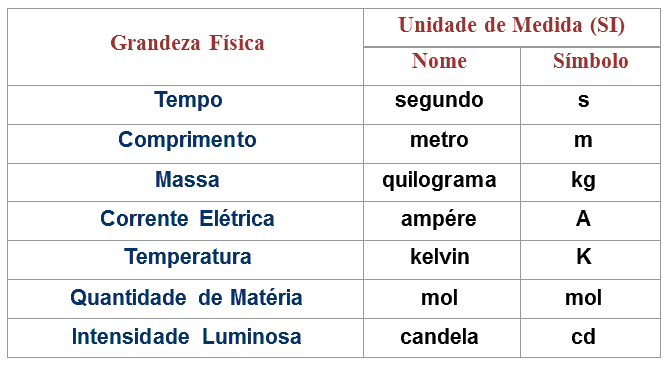
\includegraphics[scale=1]{figuras/tabela_grandeza_unidade.png}
\subsubsection{Conversão de Valores}
\begin{multicols}{2}
\begin{flushleft}
Comprimento.
\end{flushleft}
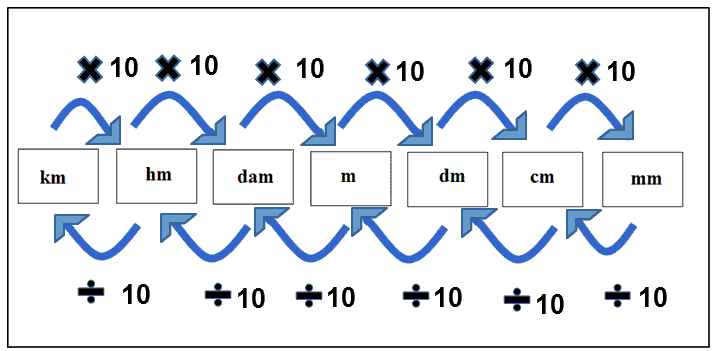
\includegraphics[scale=0.3]{figuras/conversao_comprimento.png}
\begin{flushleft}
Área.
\end{flushleft}
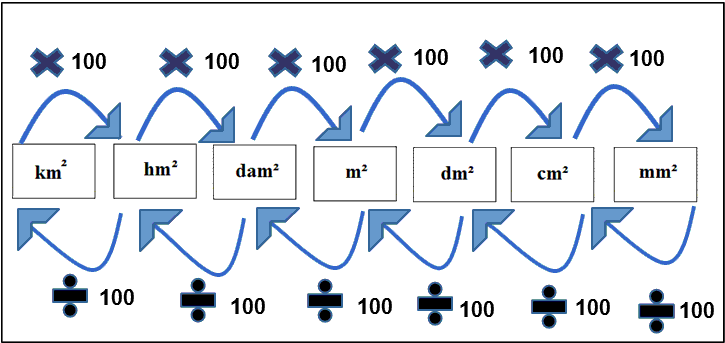
\includegraphics[scale=0.3]{figuras/conversao_area.png}
\begin{flushleft}
Massa.
\end{flushleft}
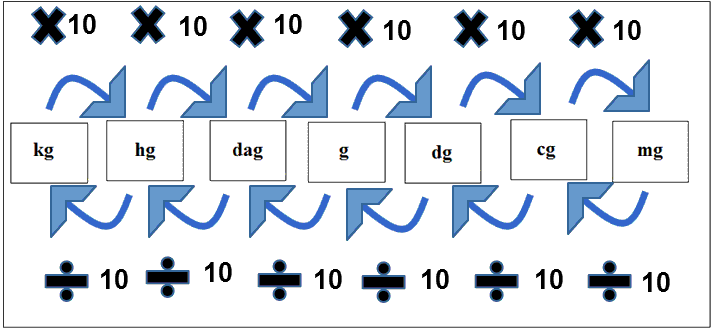
\includegraphics[scale=0.3]{figuras/conversao_massa.png}
\begin{flushleft}
Tempo.
\end{flushleft}
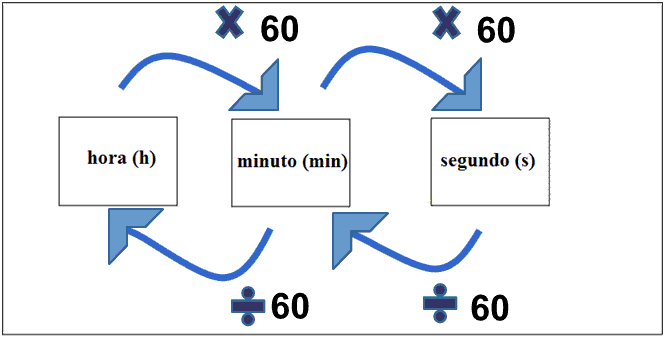
\includegraphics[scale=0.3]{figuras/conversao_tempo.png}
\end{multicols}



	\chapter{Problemas para o 8º ano}
\section{Problemas extras sobre as quatro operações.}
\begin{list}{\textbf{Questão \arabic{quest}.}}{\usecounter{quest}}
%define a margem da lista.	
%\setlength{\labelwidth}{-2mm} \setlength{\parsep}{0mm}
%\setlength{\topsep}{0mm} \setlength{\leftmargin}{-2mm}
\renewcommand{\labelenumi}{(\alph{enumi})}
	
    \item Fabrício tinha 320 reais para pagar as contas (117 reais de energia elétrica, 58 reais de água e 88 reais de telefone) e para fazer algumas compras. Quanto lhe restou para fazer as compras?
     
    \item Na escola de Pedro há 8 classes de 35 alunos, 5 classes de 33 alunos e 12 classes de 30 alunos. Qual é o total de alunos nessa escola?
     
    \item Quarenta e cinco balas foram repartidas entre 3 crianças, Ana, Maria e João. Quantas balas cada uma recebeu?
     
    \item Ana tinha 500 reais no banco. Na segunda-feira retirou 250 reais e na terça-feira fez um depósito de 180 reais. Qual o valor do seu saldo?
     
    \item Fernando comprou 4 cadernos e pagou R\$ 15,00. Quanto pagaria se tivesse comprado 12 cadernos?
     
    \item O preço de três camisetas é R\$ 54,00. Noemi deu uma nota de R\$ 50,00 para pagar a compra de duas camisetas. Quanto recebeu de troco?
     
    \item Aline tinha uma certa quantia na bolsa. Emprestou R\$ 15,00 ao seu irmão e agora tem R\$65,00. Qual quantia ela tinha inicialmente na bolsa?
     
    \item Laura e Célia jogaram uma partida de videogame em 5 rodadas. Laura fez nas três primeiras rodadas 47 pontos em cada uma e, nas seguintes, 51 e 49 pontos. Célia fez 50 pontos na primeira rodada e, nas seguintes, 48 pontos em cada uma. Responda às perguntas a seguir.
	\begin{enumerate}[a)]
    	\item Quem fez mais pontos na partida?
    	\item Quantos pontos faltaram para Laura totalizar 270 pontos?
	\end{enumerate}      
	
	\item Na escola de Pedro há 7 classes de 35 alunos, 9 classes de 33 alunos e 12 classes de 30 alunos. Qual é o total de alunos nessa escola?
	
	\item Se 65 reais é o preço de 13 cadernos, quanto pagaremos por 20 cadernos?
	
	\item Para plantar 532 mudas de rosas em 14 canteiros, com a mesma quantidade de mudas em todos eles, quantas mudas Lauro precisa colocar em cada canteiro?
	
	\item . Uma farmácia possui na prateleira um analgésico com 8 comprimidos em cada cartela. Cada caixa desse analgésico contém 25 cartelas. Na prateleira, estão 3 caixas fechadas e 1 caixa com 12 cartelas. Qual é o total de comprimidos desse analgésico?
	
	\item  Uma loja de meias possui em seu estoque 20 caixas de meias pretas, 15 caixas de meias brancas e 14 caixas de meias azuis. As caixas com meias pretas e brancas contêm 36 pares em cada caixa e as restantes, 18 pares em cada caixa. Qual é o total de meias do estoque? Quantos pares fazem parte do estoque?
	
	\item Uma fábrica de massas produz massas de pizza de dois tipos: pequena e grande. Os pacotes com pizzas pequenas contêm 10 massas cada um e os pacotes com pizzas grandes contêm 2 massas cada um. Um carregamento saiu da fábrica com 4700 pizzas entre pequenas e grandes. Sabe-se que 1180 pizzas são grandes. Quantos pacotes de pizzas pequenas e grandes estão no carregamento?
	
	\item Um conjunto habitacional possui 16 prédios, sendo 9 prédios de 6 andares cada um, com quatro apartamentos por andar, e os restantes com 5 andares cada um, com 6 apartamentos por andar. Qual é o total de apartamentos desse conjunto habitacional?
	
	\item Meu livro tem 160 páginas. Já li 92. quero terminar a leitura em 4 dias lendo o mesmo número de páginas em cada dia. Quantas páginas lerei por dia?
	
	\item Três garçons juntaram as gorjetas do dia: 70 notas de 10 reais e 22 notas de 5 reais. Dividindo igualmente esse total, quanto receberá cada um?
	
	\item Um caminhão transporta 85 sacas de café em cada viagem. Quantas viagens ele terá de fazer para transportar 680 sacas de café?
	
	\item Para uma pessoa estar bem alimentada, é recomendável que ela tome 2 copos de leite por dia. Quantos copos de leite uma pessoa deve tomar em um ano?
	
	\item Para uma pessoa estar bem alimentada, é recomendável que ela tome 2 copos de leite por dia. Quantos copos de leite uma pessoa deve tomar em um ano?
	
	\item Um prédio comercial tem 20 andares. Até o 8º andar existem 24 escritórios por andar. Nos demais, existem 13 escritórios por andar. Quantos escritórios existem até o 8º andar. Quantos escritórios existem no prédio?
	
	\item Júlia e sua prima compraram 108 carrinhos e pagaram R\$ 216,00. Deste valor sua prima pagou R\$ 126,00 pelos seus carrinhos.
	\begin{multicols}{2}
	\begin{enumerate}[a)]
		\item Qual foi o valor pago por Júlia?
		\item Quanto custa cada carrinho?
		\item Quantos carrinhos Júlia comprou?
		\item  Quantos carrinhos a prima comprou?
	\end{enumerate}
	\end{multicols}
		
	\item Um comerciante comprou por R\$ 720,00 um atum com 20 kg. Ele vendeu cada quilo de atum por R\$ 60,00.
	\begin{enumerate}[a)]
		\item Quanto o comerciante pagou por cada quilo de atum?
		\item Quanto ele faturou ao vender os 20 kg de atum?
		\item Qual foi o lucro total do comerciante ao vender os 20 kg de atum? (lembrando que lucro é o faturamento menos o valor pago pelo comerciante)
	\end{enumerate}	

	\item Dona Márcia comprou 7 dúzias de bananas. Distribuiu duas para cada macaco e ela reservou 12 para levar para casa. Quantos macacos ela alimentou?

	\item  Sílvia comprou uma geladeira por R\$ 820,00. Ela deu R\$ 220,00 de entrada e pagou o restante em três prestações mensais de igual valor. Qual o valor de cada prestação?

	\item Na decisão das Olimpíadas, foram realizadas três partidas de basquete. Na primeira partida, compareceram 2.853 pessoas. Na segunda,1.987 e, na final, 3.587 pessoas.
	\begin{enumerate}[a)]
		\item Em qual partida o público foi maior?
		\item Qual a diferença de público entre o terceiro e o primeiro jogo?
		\item Nos três jogos, quantas pessoas compareceram no total?
	\end{enumerate}

	\item Minha mãe nasceu em 1967. Eu nasci 24 anos depois. Quantos anos eu tenho agora?
	
	\item Na banca de revistas, Mariana comprou um álbum de figurinhas que custou R\$ 1,50; um pacote de figurinhas por R\$ 0,25; uma revista em quadrinhos por R\$ 2,50 e uma revista sobre informática que custou R\$4,25.De acordo com os preços, responda:
	\begin{enumerate}[a)]
		\item Quanto Mariana gastou ao todo?
		\item Se Mariana pagar a conta com uma nota de R\$ 50, quanto receberá de troco?
	\end{enumerate}
	
	\item Um camelô comprou 30 ursinhos de pelúcia por R\$ 165,00. Desejando lucrar R\$ 75,00 com a venda desses ursinhos, por quanto o camelô deve vender cada um?

	\item Um escritor escreveu, em certo dia, as 20 primeiras páginas de um livro. A partir desse dia, ele escreveu a cada dia tantas páginas quanto havia escrito no dia anterior mais 5 páginas. Se o escritor trabalhou 4 dias, quantas páginas ele escreveu no total?

	\item  A Lotação de um Teatro é de 360 lugares, todos do mesmo preço. Uma parte da lotação foi vendida por R\$ 3.000,00, tendo ficado ainda por vender ingressos no valor de R\$ 6.000,00. Quantos ingressos já foram vendidos?

	\item Um pai tem 35 anos e seus filhos 6, 7 e 9 anos. Daqui a 8 anos, a soma das idades dos três filhos menos a idade do pai será de quanto?

	\item Em uma sala de aula, onde todos os lugares se encontram ocupados, os alunos estão sentados em filas e essas filas têm todas o mesmo número de lugares.
	
	O aluno roberto tem:
	\begin{enumerate}
		\item[$-$]um aluno sentado à sua frente;
		\item[$-$]dois alunos sentados atrás de si;
		\item[$-$]três alunos sentados à sua direita;
		\item[$-$]dois alunos sentadas à sua esquerda.
	\end{enumerate}
	Quantos alunos há na sala de Roberto?	

	\item Dispomos de cinco cadeados e 5 chaves para os mesmos. Qual o número máximo de tentativas que devemos fazer para estabelecer a correspondência correta entre os cadeados e as chaves?
\end{list}
	\chapter{Problemas para o 9º ano}
\subsection{Radiciação}
\begin{list}{\textbf{Questão \arabic{quest}.}}{\usecounter{quest}}
%define a margem da lista.	
%\setlength{\labelwidth}{-2mm} \setlength{\parsep}{0mm}
%\setlength{\topsep}{0mm} \setlength{\leftmargin}{-2mm}
\renewcommand{\labelenumi}{(\alph{enumi})}

\item Calcule:
\begin{multicols}{5}
\begin{enumerate}[a)]
	\item $\sqrt{9}$
	\item $\sqrt{36}$
	\item $\sqrt{16}$
	\item $\sqrt{25}$
	\item $\sqrt{49}$

	\item $\sqrt{64}$
	\item $\sqrt{81}$
	\item $\sqrt{100}$
	\item $\sqrt{9}$
	\item $\sqrt{2}$
\end{enumerate}
\end{multicols}

\item Calcule:
\begin{multicols}{5}
\begin{enumerate}[a)]
	\item $\sqrt{144}$
	\item $\sqrt{196}$
	\item $\sqrt{324}$
	\item $\sqrt{225}$
	\item $\sqrt{289}$

	\item $\sqrt{121}$
	\item $\sqrt{400}$
	\item $\sqrt{256}$
	\item $\sqrt{625}$
	\item $\sqrt{1296}$
\end{enumerate}
\end{multicols}

\item Calcule:
\begin{multicols}{5}
\begin{enumerate}[a)]
	\item $\sqrt{0,01}$
	\item $\sqrt{0,16}$
	\item $\sqrt{1,25}$
	\item $\sqrt{2,25}$
	\item $\sqrt{2,89}$

	\item $\sqrt{1,21}$
	\item $\sqrt{12,96}$
	\item $\sqrt{2,56}$
	\item $\sqrt{6,25}$
	\item $\sqrt{1,96}$
\end{enumerate}
\end{multicols}
\end{list}
	\chapter{Números Naturais}
\section{Sistemas de numeração}
\begin{list}{\textbf{Questão \arabic{quest}.}}{\usecounter{quest}}
%define a margem da lista.	
%\setlength{\labelwidth}{-2mm} \setlength{\parsep}{0mm}
%\setlength{\topsep}{0mm} \setlength{\leftmargin}{-2mm}
\renewcommand{\labelenumi}{(\alph{enumi})}

\item Passe o número abaixo para o nosso sistema de numeração.
		\begin{multicols}{4}		
		\begin{enumerate}
			\item XX
			\item CM
			\item LXVII
			\item XLV
			\item XXXIX
			\item XIII
			\item MDCCLXXIX
			\item MCMLXIII
		\end{enumerate}
		\end{multicols}
		
		\item Escreva os números abaixo no sistema de numeração romano.
			\begin{multicols}{4}		
			\begin{enumerate}
				\item 18
				\item 352
				\item 29
				\item 734
				\item 97
				\item 3008
				\item 270
				\item 999
			\end{enumerate}
			\end{multicols}
			
		\item Passe do sistema de numeração romano para o nosso sistema.
		\begin{multicols}{3}		
		\begin{enumerate}
			\item $\overline{XXI}DCXL$
			\item $\overline{CLXX}$
			\item $\overline{\overline{CCC}}\ \overline{LXX}IV$
		\end{enumerate}
		\end{multicols}
		
		\item Qual o valor posicional no número 7 nos números abaixo?
		\begin{multicols}{3}		
		\begin{enumerate}
			\item 279
			\item 154 523 657
			\item 78 954
		\end{enumerate}
		\end{multicols}
		
		\item Escreva:			
		\begin{enumerate}
			\item Um número natural de cinco algarismo distintos no qual apareça o 2 no valor posicional 20;
			\item o menor número natural de quatro dígitos;
			\item o maior número natural de três algarismos distintos cuja a soma seja 6.
		\end{enumerate}
		
		\item O número 8 515 692 a ordem do algarismo 1 é a das dezenas de milhar e seu valor posicional é 10 000. Ainda em relação a esse número, responda.	
		\begin{enumerate}
			\item Qual é a ordem do algarismo 6? Qual o seu valor posicional?
			\item Qual é a ordem do algarismo 8? Qual o seu valor posicional?
			\item Quantas classe tem esse número?
			\item Quantas ordens tem esse número?
		\end{enumerate}
		
		\item Escreva como se leem o número abaixo.
		\begin{multicols}{4}		
		\begin{enumerate}
			\item 5 136 784
			\item 6 002 457
			\item 9 000 020
			\item 787 000 874 125
		\end{enumerate}
		\end{multicols}
		
		\item Escreva o número formado por:
		\begin{enumerate}
				\item seis dezenas de milhão, mais três centenas de milhar, mais nove dezenas.
				\item três unidades de milhão, mais cinco unidades de milhar, mais duas unidades.
		\end{enumerate}
		
		\item Represente com todos os algarismos.
		\begin{multicols}{3}		
		\begin{enumerate}
			\item 4,8 mil
			\item 3,6 milhões
			\item 2,7 bilhões.
		\end{enumerate}
		\end{multicols}
		
		\item Escreva na forma simplificada, com palavras e algarismo.
		\begin{multicols}{2}		
		\begin{enumerate}
			\item 10 400 000
			\item 13 500
			\item 2 000 500 000
			\item 8 000 000 000 000 
		\end{enumerate}
		\end{multicols}
		
		\item Escreva na forma simplificada (usando vírgula).
		\begin{multicols}{4}		
		\begin{enumerate}
			\item 9 600 000
			\item 23 500
			\item 8 600
			\item 6 600
		\end{enumerate}
		\end{multicols}
		
		\item Identifique qual ideia da adição está envolvida em cada situação e responda às questões.
		\begin{enumerate}
			\item Marcelo tinha 123 reais e ganhou de sua tia uma nota de 50 reais. Com quanto ele ficou?
			\item A coleção de Marta tem 60 adesivos e a de Aninha tem 50 adesivos. Reunindo as duas coleções, quantos adesivos elas têm?
			\item De 1º de junho a 31 de julho do mesmo ano, incluindo esses dias, quantos dias temos?
			\item Pedro já caminhou 1450 metros. Se caminhar outros 500 metros, vai completar um percurso de quantos metros?
		\end{enumerate}
		
		\item Elabore um problema que envolva uma adição.
		
		\item Use o algoritmo da decomposição para resolver a situação a seguir: Jonas tinha 624 reais na poupança e depositou 142 reais. Quanto ele tem agora de saldo na poupança?
		\item Explique com suas palavras por que o zero é chamando de elemento neutro da adição.
		
		\item No início do mês, no estoque de uma loja de brinquedos havia 2174 bonecos articulados. Durante a semana, foram vendidos 1268 bonecos. Quantos bonecos restaram?
		
		\item Efetue estas subtrações usando o algoritmo da  decomposição do subtraendo.		
		\begin{multicols}{4}
		\begin{enumerate}
			\item $497-54$
			\item $1239-129$
			\item $795-148$
			\item $2914-1825$
		\end{enumerate}
		\end{multicols}
		
		\item Um \textit{pet shop} teve, no mês de março, uma despesa de 4256 reais e um faturamento de 7250 reais. Nesse mês houve lucro ou prejuízo? De quanto?
		\item Pedro tinha 567 selos. Deu 45 para Carla, 39 para Beto e 27 para Bia. Com quantos selos ele ficou?
		\item Descubra os algarismos que faltam em cada um dos algoritmos abaixo:
		\begin{multicols}{2}
		\begin{enumerate}
			\item 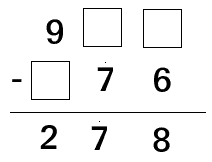
\includegraphics[scale=0.4]{figuras/fig66.png}
			\item 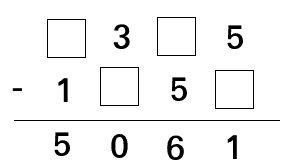
\includegraphics[scale=0.4]{figuras/fig67.png}
		\end{enumerate}
		\end{multicols}
		
\end{list}
	\chapter{Números Inteiros}

\begin{list}{\textbf{Questão \arabic{quest}.}}{\usecounter{quest}}
%define a margem da lista.	
%\setlength{\labelwidth}{-2mm} \setlength{\parsep}{0mm}
%\setlength{\topsep}{0mm} \setlength{\leftmargin}{-2mm}
\renewcommand{\labelenumi}{(\alph{enumi})}

\item Registre usando números positivos, negativos ou zero.
		\begin{enumerate}
			\item uma altitude de 50 m acima do nível do mar.
			\item a altitude de  43 m abaixo do nível do mar.
			\item a altitude ao nível do mar.
		\end{enumerate}
		
		\item Em uma cidade de Europa, foi registrada a temperatura ao meio-dia durante os oito primeiros dias de janeiro de certo ano. Veja  resultado das anotações no gráfico abaixo, que relaciona cada dia à temperatura correspondente.
		
		\begin{center}
				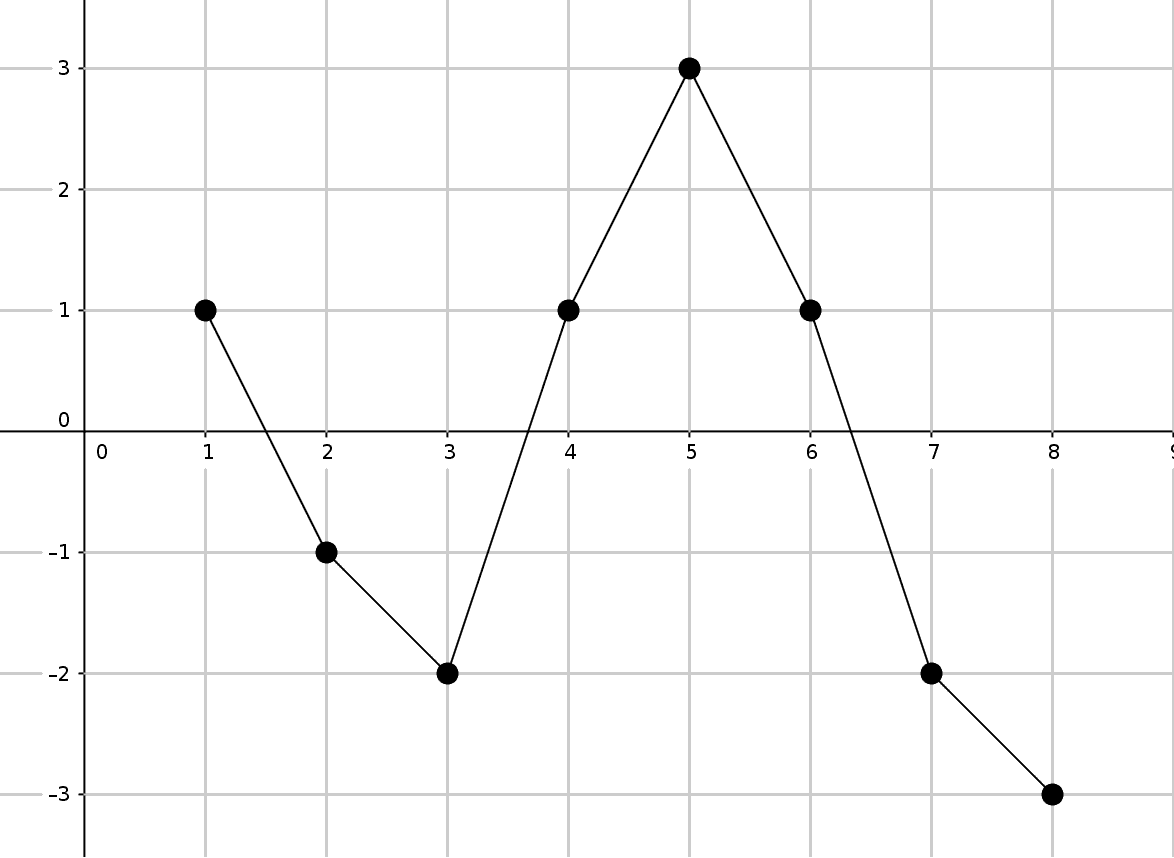
\includegraphics[scale=0.25]{figuras/fig42.png}.
		\end{center}		
		\begin{enumerate}
			\item Qual foi a temperatura máxima registrada nesses dias? Em que dia ocorreu?
			\item Qual foi temperatura mínima? Em que dia ocorreu?
			\item Em que dia a temperatura registrada foi de 0º C?
			\item Qual foi a temperatura registrada no dia 2?
		\end{enumerate}
		
		\item Localize na reta os pontos dados.
		\begin{center}
			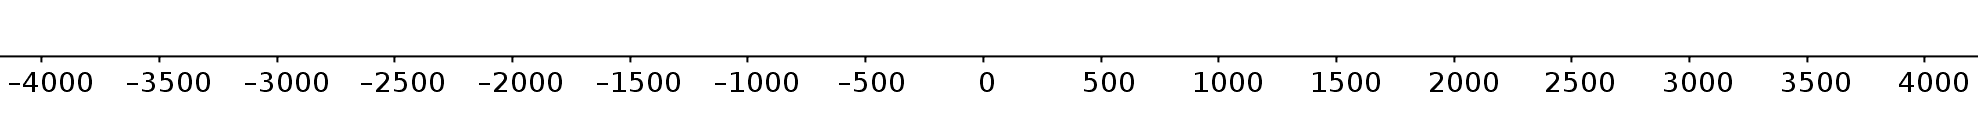
\includegraphics[scale=0.33]{figuras/fig43.png}
		\end{center}
		Coloque na reta os seguintes pontos.
		\begin{multicols}{5}
		\begin{enumerate}
			\item 476
			\item -753
			\item 391
			\item -540
			\item -405
		\end{enumerate}
		\end{multicols}
		\item Responda:
		\begin{enumerate}
			\item Em que ano morreu uma pessoa que nasceu no ano -15 e viveu 60 anos?
			\item Quantos anos viveu uma pessoa que nasceu no ano -75 e morreu no ano +5?
			\item Em que ano nasceu uma pessoa que viveu 92 anos e morreu no ano -20?
		\end{enumerate}
		
		\item Efetue a subtração correspondente a cada situação e escreva qual a temperatura resultante.		
		\begin{enumerate}
			\item A temperatura era de 18º C e baixou 4ºC.
			\item A temperatura era de 10ºC e baixou 10ºC.
			\item A temperatura era de 2ºC e baixou 5ºC.
			\item A temperatura era de 0ºC e baixou 7ºC.
		\end{enumerate}
		
		\item Considere o conjunto dos números inteiros e escreva:
		\begin{multicols}{2}		
		\begin{enumerate}
			\item o sucessor de 8.
			\item o antecessor de 0.
			\item o sucessor de 50.
			\item o sucessor de -2.
			\item o antecessor de -2.
			\item o antecessor de -69.
		\end{enumerate}
		\end{multicols}
		
		\item Coloque entre cada $\square$ o símbolo de pertence $(\in)$ ou de não pertence $(\notin)$.
		\begin{multicols}{3}
		\begin{enumerate}
			\item -6 $\square\ \mathbb{N}$ 
			\item -2 $\square\ \mathbb{Z}$ 
			\item -0 $\square\ \mathbb{Z}$
			\item 16 $\square\ \mathbb{N}$
			\item +13 $\square\ \mathbb{Z}$   
			\item 2,7 $\square\ \mathbb{Z}$ 
		\end{enumerate}		
		\end{multicols}
		
		\item Escreva:
		\begin{multicols}{2}
		\begin{enumerate}
			\item um número inteiro que não é natural.
			\item um número natural que não é inteiro.
		\end{enumerate}
		\end{multicols}
		
		\item Observe a reta numerada, a seguir, e escreva a localização dos seguintes pontos em relação à origem.
		\newline
		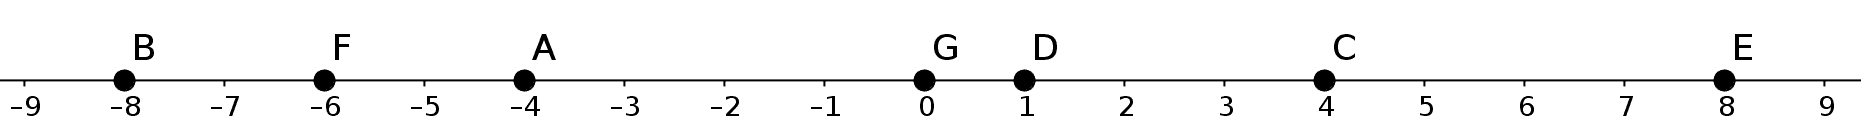
\includegraphics[scale=0.3]{figuras/fig44.png} 		
		\begin{multicols}{3}
		\begin{enumerate}
			\item A = 
			\item B = 
			\item C =
			\item D =
			\item E =
			\item F = 
		\end{enumerate}
		\end{multicols}
		
		\item Determine:
		\begin{multicols}{3}
		\begin{enumerate}
			\item |-2| 
			\item |150|
			\item |-7|
			\item |-50|
			\item |-3| + 3 + |-5|
			\item |5| + |4| + |-5|
		\end{enumerate}
		\end{multicols}
		
		\item Determine o oposto ou simétrico  de cada número.
		\begin{multicols}{3}
		\begin{enumerate}
			\item -7 
			\item 200
			\item -53
			\item 55
			\item 1 000
			\item -5 000
		\end{enumerate}
		\end{multicols}
		
		\item Complete com >, < ou = os espaços entre os números. Use o processo que julgar mais conveniente.
		\begin{multicols}{4}
		\begin{enumerate}
			\item 86 \ \ -100
			\item 623 \ \ 519
			\item -374 \ \ -200
			\item 0 \ \ -6
			\item 0 \ \ 11
			\item +8 \ \ 8
			\item +4 \ \ -4
			\item -6 \ \ +2
			\item +6 \ \ -2
			\item -18 \ \ 0
			\item +16 \ \ 0
			\item -3 \ \ +9
		\end{enumerate}
		\end{multicols}
		
		\item Efetue as adições.
		\begin{multicols}{3}
		\begin{enumerate}
			\item $-2-2$
			\item $(-3)+(+3)$
			\item $+2-0$
			\item $(-3)+(+3)$
			\item $+2-0$
			\item $+4-6$
			\item $(-5)+(+7)$
			\item $(-3)+(-4)$
			\item $(+3) +0$
			\item $+6+1$
			\item $+5-4$
			\item $(-12)+(-15)$
			\item $ +23+30$
			\item $(+17)+(+49)$
			\item $-132-29$
			\item $(+51)+(-51)$
			\item $-80+30$
			\item $-27+30$
			\item $(+230)+(-201)$
			\item $-37+37$
			\item $+46-59$
		\end{enumerate}
		\end{multicols}
		
		\item Escreva e efetue a adição correspondente a cada situação e indique o novo saldo.
		\begin{enumerate}
			\item O saldo de José era negativo de R\$ 150,00 e ele fez um depósito de R\$ 200,00.
			\item O saldo de Ana era positivo de R\$ 95,00, e ela realizou uma retirada de R\$ 150,00.
			\item O saldo de Sílvio era negativo de R\$ 55,00, e ele efetuou uma retirada de R\$ 60,00.
			\item O saldo de Sueli era zero, e ela fez um depósito de R\$ 300,00.
			\item O saldo de Sérgio era positivo de R\$ 427,00, e ele realizou um depósito de R\$ 248,00.
		\end{enumerate}
		
		\item Use o processo que julgar mais conveniente, como estudado nas aulas, e calcule:
		\begin{multicols}{2}
		\begin{enumerate}
			\item $-12+4+11-8+13 +1$
			\item $(+6)+(-14)+(-7)+(6)+(+9)$
			\item $-2+5+3-2+1$
			\item $-7-3-9+8-1-4$
			\item $(+16)+(-29)+(+33)+(-37)$
			\item $(-3)+(-5)+(-2)+(-1)$
		\end{enumerate}
		\end{multicols}
		
		\item Vamos imaginar o movimento de um elevador em um prédio de 8 andares (acima do térreo) e 3 subsolos, como indica a figura ao lado. Complete a tabela abaixo. Na última coluna, indique a operação efetuada (adição ou subtração.)
		\newline
		\newline
		\begin{tabular}{|c|c|c|c|}
		\hline 
		Andar da saída & Deslocamento do elevador & Andar de chegada & Operação efetuada \\ 
		\hline 
		-1 & +3 &   &   \\ 
		\hline 
		-2 & -1 &   &   \\ 
		\hline 
		+3 &   & -3 &   \\ 
		\hline 
		  & +2 & +2 &   \\ 
		\hline 
		0 & -2 &   &   \\ 
		\hline 
		-3 &   & -1 &   \\ 
		\hline 
		\end{tabular} 
		
		\item Efetue estas multiplicações que envolvem todos os casos estudados.
		\begin{multicols}{3}
		\begin{enumerate}
			\item $(-7)\cdot(-11)$
			\item $(+4)\cdot(+3)$
			\item $(-14)\cdot0$
			\item $(-8)\cdot(+9)$
			\item $0\cdot(-342)$
			\item $(+12)\cdot(-12)$
		\end{enumerate}
		\end{multicols}
		
		\item Calcule:
		\begin{multicols}{4}
		\begin{enumerate}
			\item $(2)^5$
			\item $(+10)^{10}$
			\item $(-3)^4$
			\item $(-2)^5$
			\item $(+1)^3$
			\item $(+1)^2$
			\item $(-1)^5$
			\item $(-1)^4$
		\end{enumerate}
		\end{multicols}
\end{list}
	\chapter{Cálculo Numérico}
\section{Operações com números reais.}
\begin{list}{\textbf{Questão \arabic{quest}.}}{\usecounter{quest}}
%define a margem da lista.	
%\setlength{\labelwidth}{-2mm} \setlength{\parsep}{0mm}
%\setlength{\topsep}{0mm} \setlength{\leftmargin}{-2mm}
\renewcommand{\labelenumi}{(\alph{enumi})}

\item Calcular o valor numérico de cada expressão.
\begin{multicols}{2}
\begin{enumerate}

	\item $\displaystyle{
			\frac{\displaystyle{\frac{4}{5}-\frac{1}{2}}}{\displaystyle{\left(\frac{3}{2}\right)^{-2}}}
			}$
	\item $0,2-\left\{(0,5)^2\cdot(-2)+\left[3:(4^0\cdot\sqrt{36})\right]-1\right\}$
\end{enumerate}
\end{multicols}
	\item Dar o valor da expressão 
		$\displaystyle{
		\frac{10^{-2}+\sqrt{400}-(8,1:3)^{3}}
		{\displaystyle\sqrt[10]{1024}-\left(\displaystyle\frac{13}{4}\right)^0}
		}$.
	\item Racionalizar o denominador da fração $\displaystyle{\frac{\sqrt{2}+2}{\sqrt{2}-2}}$.
	\item Calcular o valor da raiz quadrada de $82,81$.
	\item Calcular $12\%$ de $75\%$ de 36.

	\item Calcule o valor de cada expressão.
	%\begin{multicols}{2}
	\begin{enumerate}
		\item $\displaystyle{
			1,8 + \left\{ 13 - (5^2-3):\left[3-(0,9)^0\right]\right\}+\sqrt{0,36}
			}$
		\item $\displaystyle{
			\frac{\displaystyle\frac{1}{3}+\frac{4}{5}}{\displaystyle\frac{2}{9}\cdot\frac{3}{2}}		
		}$
		\item $\displaystyle{
			\frac{\displaystyle\frac{2}{3}\cdot\frac{1}{7}}{\displaystyle\frac{1}{5}\cdot\left(\frac{3}{10}\right)^{-1}}		
		}$
		\item $\left[3,2\cdot(0,8)^{-2}+5\right]:0,2+\left[(-5,2)^0:0,3\right]^{-1}$
		\item $\displaystyle{
			\left(\frac{1}{3}\right)^{2} + \left(\frac{3}{4}\right)^{-2} \cdot \left(\frac{2}{5}\right)^{-1}	
		}$
		\item $\frac{\displaystyle\frac{5}{3}\cdot(2,1)}{\displaystyle(6,4):\displaystyle\left(\frac{6}{4}\right)}$
		\item $\displaystyle\frac{\displaystyle\frac{2}{3}+ (0,3)^{-1}}{2,7\cdot\displaystyle\frac{1}{9}} : \frac{5:0,2}{3-\displaystyle\frac{1}{2}}$
	\end{enumerate}
	%\end{multicols}
	\item Calcule o valor das expressões.
	\begin{enumerate}
		\item $\displaystyle\frac{\sqrt{169}-(0,2:2)+10^0} {\left( \displaystyle\frac{2}{5} \cdot \frac{1}{6}\right)-\sqrt[5]{25 \cdot 125}}$ 
		\item $\displaystyle\frac{(-2,1+3\cdot 1,2) + (0,05:0,1)^{-1}}{\left[(-2)^2:(-2)^3\right]^{-1}}+\sqrt{196}$
	\end{enumerate}
	\item Dividir um número por 0,0625 é equivalente a multiplicá-lo por:
	\begin{multicols}{5}
	\begin{enumerate}
		\item 4
		\item 8
		\item 16
		\item 2
		\item 1
	\end{enumerate}
	\end{multicols}
	\item Racionalize o denominador das expressões.
	\begin{multicols}{2}
	\begin{enumerate}
		\item $\displaystyle\frac{2}{\sqrt{3}}$
		\item $\displaystyle\frac{2}{\sqrt{7}-\sqrt{5}}$
		\item $\displaystyle\frac{3}{2+\sqrt{3}}$
		\item $\displaystyle\frac{\sqrt{11} + \sqrt{7}}{\sqrt{11} - \sqrt{7}}$
		\item $\displaystyle\frac{6}{\sqrt[3]{3}}$
		\item $\displaystyle\frac{10}{\sqrt[4]{8}}$
	\end{enumerate}
	\end{multicols}
	\item Calcule os valor das expressões.
	\begin{multicols}{2}
	\begin{enumerate}
		\item $\sqrt{289}+\sqrt{441}$
		\item $\sqrt[4]{1296}-\sqrt[5]{243}$
		\item $\sqrt{72}+\sqrt{50}$
		\item $\displaystyle\frac{7}{\sqrt[3]{729}} + \frac{3}{\sqrt[7]{128}}$
		\item $\displaystyle\sqrt[4]{32} + \sqrt[3]{40} - \sqrt[4]{162}$
	\end{enumerate}
	\end{multicols}
	\item Calcule:
	\begin{multicols}{2}
	\begin{enumerate}
		\item 20\% de 450.
		\item 35\% de 800
		\item 1\% de 10\% de 9
		\item $(25\%)^2$ de 100
	\end{enumerate}
	\end{multicols}
\end{list}	
	\chapter{Cálculo Algébrico}
\section{Fatoração e simplificação de expressões algébricas}
\begin{list}{\textbf{Questão \arabic{quest}.}}{\usecounter{quest}}
%define a margem da lista.	
%\setlength{\labelwidth}{-2mm} \setlength{\parsep}{0mm}
%\setlength{\topsep}{0mm} \setlength{\leftmargin}{-2mm}
\renewcommand{\labelenumi}{(\alph{enumi})}

\item Desenvolver as expressões algébricas.
	\begin{multicols}{3}
	 \begin{enumerate}
	 	\item $(y-4)^2$
	 	\item $(5p-4q)\cdot (5p+4q)$
	 	\item $(z-2)^3$
	 \end{enumerate}
	 \end{multicols}
	 \item Fatorar as expressões algébricas.
	 \begin{multicols}{3}
	 \begin{enumerate}
	 	\item $21x^2+18x+3xz$
	 	\item $xy +2x+ 5y+ 10$
	 	\item $16z^2 - 4t^2$
	 	\item $y^2 + 6y +9$
	 	\item $m^3 - 27$
	 	\item $n^3+8$
	 \end{enumerate}
	 \end{multicols}
	 \item Desenvolva as expressões algébricas.
	\begin{multicols}{2}	 
	 \begin{enumerate}
	 	\item $(2x+ 5)^2$
	 	\item $\left(3x^3 + \displaystyle\frac{y}{4}\right)^2$
	 	\item $(7 - 4y)^2$
	 	\item $\left(\displaystyle\frac{m}{2} - \frac{n}{3}\right)^2$
	 	\item $(2p+3z)(2p-3z)$
	 	\item $\left(\displaystyle\frac{x}{2} + \frac{5y}{3}\right)\left(\displaystyle\frac{x}{2} - \frac{5y}{3}\right)$
	 	\item $(4+q)^3$
	 	\item $(y-2)^3$
	 \end{enumerate}
	 \end{multicols}
	 \item Simplifique as expressões algébricas:
	 \begin{multicols}{2}	 
	 \begin{enumerate}
	 	\item $x(3x + 1) + (x + 2)^2$
	 	\item $(y + 1) (y - 1) - (y + 3)^2$
	 	\item $(2 + z)^3 - 2(4 + 3z)$
	 	\item $(4p + 3)^2 + (2p - 2)^2$
	 	\item $(2y - 1)(z - 2) - 2$
	 	\item $(2 - m)^2 - m^2 + 4$ 
	 \end{enumerate}
	 \end{multicols}
	 \item Fatore as expressões algébricas:
	 \begin{multicols}{3}
	 \begin{enumerate}
	 	\item $\displaystyle\frac{z}{6} + \frac{xz}{8} + \frac{yz^2}{12}$
	 	\item $8z + 32y^2z + 20yz^2$
	 	\item $\displaystyle\frac{8}{ab^3} + \frac{4}{ab^2} - \frac{20}{a^3b^2}$
	 	\item $3q + 6 + pq + 2p$
	 	\item $xy + 2x + \displaystyle\frac{y}{4} + \frac{1}{2}$
	 	\item $px + qx - p - q$
	 	\item $y^{16} - x^{16}$
	 	\item $4m^2 - 36n^2$
	 	\item $\displaystyle\frac{a^2b^6}{64} - \frac{49}{a^{10}}$
	 	\item $9z^2 + 6z + 1$
	 	\item $64 + n^3$
	 	\item $8 - 216z^3$
	 \end{enumerate}
	 \end{multicols}
\end{list}

\section{Simplificação de frações algébricas}
\begin{list}{\textbf{Questão \arabic{quest}.}}{\usecounter{quest}}
%define a margem da lista.	
%\setlength{\labelwidth}{-2mm} \setlength{\parsep}{0mm}
%\setlength{\topsep}{0mm} \setlength{\leftmargin}{-2mm}
\renewcommand{\labelenumi}{(\alph{enumi})}

	\item simplificar as frações algébricas.
	\begin{multicols}{3}
	\begin{enumerate}
		\item $\displaystyle\frac{12x^2 - 6x}{6x}$
		\item $\displaystyle\frac{y^2 - 9}{y^2 + 6y +9}$
		\item $\displaystyle\frac{z - zx + 3 - 3x}{1 - x}$
	\end{enumerate}
	\end{multicols}
\end{list}
	\chapter{Porcentagem}
\begin{list}{\textbf{Questão \arabic{quest}.}}{\usecounter{quest}}
%define a margem da lista.	
%\setlength{\labelwidth}{-2mm} \setlength{\parsep}{0mm}
%\setlength{\topsep}{0mm} \setlength{\leftmargin}{-2mm}
\renewcommand{\labelenumi}{(\alph{enumi})}

\item Calcule:
\begin{multicols}{4}
\begin{enumerate}
	\item 15\% de 300
	\item 80\% de 1 200 
	\item 9\% de 50 000
	\item 31\% de 2 500 
	\item 43\% de 7 200 
	\item 91\% de 9 400
	\item 8\% de 32 500
	\item 67\% de 20 000 
\end{enumerate}
\end{multicols}

\item Na minha cidade, foi feita uma pesquisa sobre o meio de transporte utilizado pelos alunos para chegarem  à  escola. Responderam  à  essa  pergunta  2000  alunos.  42\%  responderam  que  vão  de  carro,  25\% responderam que vão de moto, e o restante de ônibus. Calcule todas as porcentagens possíveis. 

\item Ao  comprar  um  produto  que  custava  R\$ 1.500,00  obtive  um  desconto  de  12\%.  Por  quanto acabei pagando o produto? Qual o valor do desconto obtido?

\item Na  festa  de  aniversário  do  meu  sobrinho  derrubei  uma  mesa  onde  estavam  40  garrafas  de refrigerante.  Sobraram  apenas  15\%  das  garrafas  sem quebrar.  Quantas  garrafas  sobraram  e  quantas  eu quebrei?

\item Dos  28  bombons  que  estavam  na  minha  gaveta,  já  comi   75\%.  Quantos  bombons  ainda  me restam?

\item Comprei  30 peças  de roupa  para revender.  Na primeira  saída  eu  estava  com  sorte  e  consegui vender 60\%. Quantas peças de roupa eu vendi?     

\item Em  uma  população  de  250  ratos,  temos  que  16\%  são  brancos.  Qual  é  o  número  de  ratos brancos desta população?

\item Das 20 moedas que possuo em meu bolso, apenas 15\% delas são moedas de um real. Quantas moedas de um real eu possuo em meu bolso? 

\item Dos 8 irmãos que possuo, apenas 50\% são mulheres. Quantas irmãs eu possuo?

\item Um jogador de futebol, ao longo de um campeonato, cobrou 75 faltas, transformando em gols 8\% dessas faltas. Quantos gols de falta esse jogador fez?  

\item Uma loja lança uma promoção de 10\% no preço dos seu s produtos. Se uma mercadoria custa R\$120,00, quanto a mercadoria passará a custar? 

\item Com  10  kg  de  trigo  podemos  fabricar  7 kg  de  farinha.  Quantos  quilogramas  de  trigo  são necessários para fabricar 28 kg de farinha? 

\item Com 50 kg de milho, obtemos 35 kg de fubá. Quantas sacas de 60 kg de fubá podemos obter com 1 200 kg de milho?

\item Sete litros de leite dão 1,5 quilos de manteiga. Quantos litros de leite serão necessários para se obterem 9 quilos de manteiga?
\end{list}
	%Data da última atilaização: 19/10/2016
\chapter{Equações do Primeiro Grau.} \label{cap1}
		\section{Atividades Básicas}				
			\begin{list}{\textbf{Questão \arabic{quest}.}}{\usecounter{quest}}
%define a margem da lista.	
%\setlength{\labelwidth}{-2mm} \setlength{\parsep}{0mm}
%\setlength{\topsep}{0mm} \setlength{\leftmargin}{-2mm}
\renewcommand{\labelenumi}{(\alph{enumi})}
				
				\item Dada a equação $7x-3+x=5-2x$, responda.
					\setlength{\columnsep}{5pt}%define o espaçamento entre as colunas								
					\begin{multicols}{2}					
					\begin{enumerate}
						\item Qual é o primeiro membro?
						\item Qual é o segundo membro?
						\item Quais são os termos do primeiro termo?
						\item Quais são os termos do segundo termo?
					\end{enumerate}
					\end{multicols}
						
				\item Qual é o número que colocado no lugar de $x$, torna verdadeira as sentenças?
					\begin{multicols}{4}
					\begin{enumerate}
						\item $x+9=13$
						\item $x-7=10$
						\item $5x-1=9$
						\item $x-3=8$
					\end{enumerate}
					\end{multicols}
				\item Resolva as equações:
					\begin{multicols}{4}
					\begin{enumerate}
						\item $x+5=8$
						\item $x-4=3$
						\item $x+6=5$
						\item $x-7=7$
						\item $x+9=-1$
						\item $x+28=11$
						\item $x-109=5$
						\item $x-39=-79$
						\item $10=x+8$
						\item $15=x+20$
						\item $4=x-10$
						\item $7=x+8$
						\item $0=x+12$
						\item $-3=x+10$
					\end{enumerate}
					\end{multicols}
				\item Resolva:
					\begin{multicols}{4}
					\begin{enumerate}
						\item $-x=9$
						\item $-x=-2$
						\item $-7x=14$
						\item $-3x=10$
						\item $-5x=-12$
						\item $-4x=8$
						\item $-3x=-9$
						\item $-5x=15$
						\item $-2x=-10$
						\item $15=-3x$
						\item $-40=-5x$
										    
				    \end{enumerate}	
				    \end{multicols}								
				
				
				\item Resolva as seguintes equações:
					\begin{multicols}{4}					
					\begin{enumerate}
						\item $3x=15$
						\item $2x=14$
						\item $4x=-12$
						\item $7x=-21$
						\item $13x=13$
						\item $9x=-9$
						\item $25x=0$
						\item $35x=-105$
						\item $4x=1$
						\item $36x=12$
						\item $21=3x$
						\item $84=6x$
					\end{enumerate}							
					\end{multicols}
				\item Resolva as equações:
					\begin{multicols}{3}
					\begin{enumerate}
						\item $\displaystyle\frac{x}{3}=7$
						\item $\displaystyle\frac{x}{4}=-3$
						\item $\displaystyle\frac{2x}{5}=4$
						\item $\displaystyle\frac{2x}{3}=-10$
						\item $\displaystyle\frac{3x}{4}=30$
						\item $\displaystyle\frac{2x}{5}=-18$
					\end{enumerate}
					\end{multicols}				
							
				\item Resolva as equações a seguir:
					\begin{multicols}{2}
					\begin{enumerate}
						\item $18x - 43 = 65$
						\item $23x - 16 = 14 - 17x$
						\item $10y - 5 (1 + y) = 3 (2y - 2) - 20$
						\item $x(x + 4) + x(x + 2) = 2x^2 + 12$
						\item $\displaystyle\frac{(x - 5)}{10} + \frac{(1 - 2x)}{5} = \frac{(3-x)}{4}$                                 
						\item $4x (x + 6) + x^2 = 5x^2$
					\end{enumerate}				
					\end{multicols}
				\item Verifique se $1$ é a raiz da equação $\displaystyle{4x + \frac{1}{2} = \frac{9}{2}}$
						
%marcador				
       			\item Determine um número real $a$ para que as expressões $\frac{3a + 6}{8}$ e $\frac{2a + 10}{6}$ sejam iguais.
       			\item Resolver as seguintes equações (na incógnita $x$):
					\begin{multicols}{2}					
					\begin{enumerate}
		 			\item $\displaystyle\frac{5}{x} - 2 = \frac{1}{4} (x\neq 0)$
		 			\item $3bx + 6bc = 7bx + 3bc$
		 			\end{enumerate} 
		 			\end{multicols}
		 		\item Determine o valor de $x$ na equação a seguir aplicando as técnicas resolutivas.
		 			\begin{multicols}{2}
		 			\begin{enumerate}
		 				\item $3 - 2(x + 3) = x - 18$
		 				\item $50 + (3x - 4) = 2  (3x - 4) + 26$
		 			\end{enumerate}
		 			\end{multicols}
		 		\item Qual é a raiz da equação $7x - 2 = -4x + 5$?
		 		\item Resolva as Equações em $\mathbb{R}$.
		 			\begin{multicols}{2}
		 			\begin{enumerate}
		 				 \item $2x + 6 = x + 18$
		 				 \item $5x - 3 = 2x + 9$
		 				 \item $3(2x - 3) + 2(x + 1) = 3x + 18$
		 				 \item $2x + 3(x - 5) = 4x + 9$
		 				 \item $2(x + 1) - 3(2x - 5) = 6x - 3$
		 				 \item $3x - 5 = x - 2$
		 				 \item $3x - 5 = 13$
		 				 \item $3x + 5 = 2$
		 				 \item $x - (2x - 1) = 23$
		 				 \item $2x - (x - 1) = 5 - (x - 3)$   
		 			\end{enumerate}
		 			\end{multicols}
		 		\item O valor numérico da expressão $2x^2 + 8$, para $x$ igual a $-3$ é:		
		 			\setlength{\columnseprule}{0pt}
					\begin{multicols}{4}					
					\begin{enumerate}
						\item 17
						\item 18
						\item 26   
						\item 34
					\end{enumerate}
					\end{multicols}
				\item Resolva as equações.
					\setlength{\columnseprule}{0pt}
					\setlength{\columnsep}{20pt}					
					\begin{multicols}{4}
					\begin{enumerate}
						\item $2x - 3 = 15                                                   $
						\item $4y = 30 - 18                                                 $
						\item $5z - 6 = z + 14                                              $
						\item $m + 4 = 20 $
					\end{enumerate}
					\end{multicols}
				\item Resolva– as equações
					\begin{multicols}{2}
					\begin{enumerate}
						\item $4x-1=3(x-1)$
						\item $3(x-2)=2x-4$
						\item $2(x-1)=3x-4$
						\item– $3(x-1)-7=15$
						\item $7(x-4)=2x-3$
						\item $3(x-2)=4(3-x)$
						\item $3(3x-1)=2(3x+2)$
						\item $7(x-2)=5(x+3)$
						\item $3(2x-1)=-2(x+3)$
						\item $5x-3(x+2)=15$
						\item $2x+3x+9=8(6-x)$
						\item $4(x-10)-2(x-5)=0$
						\item $3(2x+3)-4(x-1)=3$
						\item $7(x-1)-2(x-5)=x-5$
						\item $2(3-x)=3(x-4)+15$
						\item $3(5-x)-3(1-2x)=42$
						\item $(4x+6)-2x=(x-6)+10+14$
						\item $(x-3)-(x+2)+2(x-1)-5=0$
						\item $3x-2(4x-3)=2-3(x-1)$
						\item $3(x-1)-(x-3)+5(x-2)=18$
						\item $5(x-3)-4(x+2)=2+3(1-2x)$
					\end{enumerate}
					\end{multicols}
				\item Resolva as seguintes equações:
					\begin{multicols}{3}
					\begin{enumerate}
						\item $\displaystyle\frac{x}{4}-\frac{x}{6}=3$
						\item $\displaystyle\frac{3x}{4}-\frac{x}{3}=5$
						\item $\displaystyle\frac{x}{5}-1=9$
						\item $\displaystyle\frac{x}{3}-5=0$
						\item $\displaystyle\frac{x}{2}+\frac{3x}{5}=6$
						\item $\displaystyle\frac{x}{5}+\frac{x}{2}=\frac{7}{10}$
						\item $5x-10=\displaystyle\frac{x+1}{2}$
						\item $\displaystyle\frac{8x-1}{x}-2x=3$
						\item $\displaystyle\frac{2x-7}{5}=\frac{x+2}{3}$
						\item $\displaystyle\frac{5x}{2}=2x+\frac{x-2}{3}$
						\item $\displaystyle\frac{x-3}{4}-\frac{2x-1}{5}=5$
						\item $\displaystyle\frac{x-1}{2}+\frac{x-3}{3}=6$
						\item $\displaystyle\frac{5x-7}{2}=\frac{1}{2}+x$
						\item $\displaystyle\frac{2x-1}{3}=x-\frac{x-1}{5}$
						\item $\displaystyle\frac{x}{4}+\frac{3x-2}{2}=\frac{x-3}{2}$
						\item $\displaystyle\frac{2(x-1)}{3}=\frac{3x+6}{5}$
						\item $\displaystyle\frac{3(x-5)}{6}+\frac{2x}{4}=7$
						\item $\displaystyle\frac{x}{5}-2=\frac{5(x-3)}{4}$
					\end{enumerate}
					\end{multicols}					
			\end{list}	
		\section{Problemas Envolvendo Equações}
			\begin{list}{\textbf{Questão \arabic{quest}.}}{\usecounter{quest}}
%define a margem da lista.	
%\setlength{\labelwidth}{-2mm} \setlength{\parsep}{0mm}
%\setlength{\topsep}{0mm} \setlength{\leftmargin}{-2mm}
\renewcommand{\labelenumi}{(\alph{enumi})}

				\item Resolva cada situação problema a seguir, utilizando equações do primeiro grau com uma variável:
					\begin{enumerate}
						\item O triplo de um número somado a quatro é igual a vinte e cinco. Qual é este número?
						\item O quíntuplo do número de meninas da 7$^{a}$A menos cinco é igual a 25. Quantas são as meninas da 7$^{a}$ A

						\item A diferença entre o triplo de um número e 90 é igual a esse número somado com 48. Que número é esse?

						\item Um número menos 12 é igual a 3/4 do mesmo número. Qual é esse número?

						\item O triplo de um número menos 40 é igual a sua metade mais 20. Que número é esse?

						\item A metade de um número mais 10 e mais a sua terça parte é igual ao próprio número. Que número é esse?

						\item Sabe-se que 3/5 da idade de Jurandir menos 15 é igual a 9. Qual é a idade de Jurandir?

						\item Um número é o triplo do outro. Somando os dois, obtemos 84. Quais são esses números?

						\item A idade de um pai é o triplo da idade de seu filho. Calcule essas idades, sabendo que juntos eles possuem 72 anos.

						\item Somando 5 anos ao dobro da idade de Sônia, obtemos 35 anos. Qual é a idade da Sônia?						

						\item Um número tem 4 unidades a mais que o outro. A soma deles é 150. Quais são estes números?						

						\item Tenho 9 anos a mais que meu irmão e juntos temos 79 anos. Quantos anos eu tenho?

						\item As idades de 3 irmão somam 99 anos. Sabendo-se que o mais jovem tem 1/3 da idade do mais velho e o 2$^{o}$ irmão tem a metade da idade do mais velho, determine a idade do mais velho.

						\item Numa escola 1/3 dos alunos são meninos e 120 são meninas. Quantos alunos há nesta escola?

						\item Numa caixa há bolas brancas e bolas pretas num total de 360. Se o número de bolas brancas é o quádruplo do número de bolas pretas, qual é o número de bolas brancas?

						\item Diminuindo-se 6 anos da idade de minha filha obtém-se os 3/5 de sua idade. Qual é a idade de minha filha?

						\item A soma de três números é 150. O segundo é o triplo do primeiro e o terceiro tem 10 unidades a mais do que o segundo. Quais são estes números?

						\item A quantidade de figurinhas que os irmão Pedro, João e Marcos possuem, somam 142. João tem o quádruplo de figurinhas de Pedro e Marcos o triplo das de João e mais seis figurinhas. Quantas figurinhas tem cada um?

						\item A soma das idades de três irmãos é 28 anos. Quando o segundo nasceu, o primeiro tinha três anos, e quando o terceiro nasceu, o segundo tinha 2 anos. Qual é a idade atual de cada um?

						\item Num campeonato de futebol, as três primeiras equipes classificadas A, B e C,  marcaram 115 gols. A equipe A marcou 12 gols a mais que a equipe C e oito gols a mais que a equipe B. Quantos gols marcou cada equipe?

						\item Jair e Edson têm juntos 35 mil reais. Jair tem a mais que Edson 6 mil reais. Quanto tem cada um?

						\item Ary e Rui têm juntos 840 reais. A quantia de Ary é igual a 3/4 da quantia de Rui. Quantos reais Rui tem?

						\item Numa partida de basquetebol, as duas equipes fizeram um total de 145 pontos. A equipe A fez o dobro de pontos menos cinco, que a equipe B. Quantos pontos marcou cada equipe? 
					\end{enumerate}
				\item O dobro de um número, aumentado de 15, é igual a 49. Qual é esse número?
				\item A soma de um número com o seu triplo é igual a 48. Qual é esse número?
				\item A idade de um pai é igual ao triplo da idade de seu filho. Calcule essas idades, sabendo que juntos têm 60 anos?
				\item Somando 5 anos ao dobro da idade de Sônia, obtemos 35 anos. Qual é a idade de Sônia?
				\item O dobro de um número, diminuído de 4, é igual a esse número aumentado de 1. Qual é esse número?
				\item O triplo de um número, mais dois, é igual ao próprio número menos quatro. Qual é esse número?
				\item O quádruplo de um número, diminuído de 10, é igual ao dobro desse número, aumentado de 2. Qual é esse número?
				\item O triplo de um número, menos 25, é igual ao próprio número, mais 55. Qual é esse número?				
				\item Um número somado com sua quarta parte é igual a 80. Qual é esse número?
				\item Um número mais a sua metade é igual a 15. Qual é esse número?
				\item A diferença entre um número e sua quinta parte é igual a 32. Qual é esse número?
				\item O triplo de um número é igual a sua metade mais 10. Qual é esse número?
				\item O dobro de um número, menos 10, é igual à sua metade, mais 50. Qual é esse número?
				\item A diferença entre o triplo de um número e a metade desse número é 35. Qual é esse número?
				\item Subtraindo 5 da terça parte de um número, obtém-se o resultado 15. Qual é esse número?
				\item A metade dos objetos de uma caixa mais a terça parte desses objetos é igual a 25. Quantos objetos há na caixa?
				\item Em uma fábrica, um terço dos empregados são estrangeiros e 72 empregados são brasileiros. Quantos são os empregados da fábrica?
				\item Flávia e Sílvia têm juntas 21 anos. A idade de Sílvia é três quartos da idade de Flávia. Qual a idade de cada uma?
				\item A soma das idades de Carlos e Mário é 40 anos. A idade de Carlos é três quintos da idade de Mário. Qual a idade de Mário?
				\item A diferença entre um número e os seus dois quintos é igual a trinta e seis. Qual é esse número?
				\item A diferença entre os dois terços de um número e sua metade é igual a seis. Qual é esse número?
				\item Os três quintos de um número aumentados de doze são iguais aos cinco sétimos desse número. Qual é esse número?
				\item Dois quintos do meu salário são reservados para o aluguel e a metade é gasta com alimentação, restando ainda R\$ 45,00 para gastos diversos. Qual é o meu salário?
				\item Lúcio comprou uma camisa que foi paga em 3 prestações. Na 1$^{\underline{a}}$ prestação, ele pagou a metade do valor da camisa, na 2$^{\underline{a}}$ prestação, a terça parte e na última, R\$ 2,00. Quanto ele pagou pela camisa?
				\item Achar um número, sabendo-se que a soma de seus quocientes por 2, por 3 e por 5 é 124.
				\item Um número tem 6 unidades a mais que outro. A soma deles é 76. Quais são esses números?
				\item Um número tem 4 unidades a mais que o outro. A soma deles é 150. Quais são esses números?
				\item Fábia tem cinco anos a mais que Marcela. A soma da idade de ambas é igual a 39 anos. Qual é a idade de cada uma?
				\item Marcos e Plínio tem juntos R\$ 350,00. Marcos tem a mais que Plínio R\$ 60,00. Quanto tem cada um?
				\item Tenho nove anos a mais que meu irmão, e juntos temos 79 anos. Quantos anos eu tenho?
				\item O perímetro de um retângulo mede 74 cm. Quais são suas medidas, sabendo-se que o comprimento tem cinco centímetros a mais que a largura?
				\item Eu tenho R\$ 20,00 a mais que Paulo e Mario R\$ 14,00 a menos que Paulo. Nós temos juntos R\$ 156,00. Quantos reais tem cada um?
				\item A soma de dois números consecutivos é 51. Quais são esses números?
				\item A soma de dois números consecutivos é igual a 145. Quais são esses números?
				\item A soma de um número com seu sucessor é 71. Qual é esse número?
				\item A soma de três números consecutivos é igual a 54. Quais são esses números?
				\item A soma de dois números inteiros e consecutivos é - 31. Quais são esses números?
				\item A soma de dois números ímpares consecutivos é 264. Quais são esses números?	
				\item Carlos tem 17 anos e Mário tem 15 anos. Daqui a quantos anos a soma de suas idades será 72 anos?
				\item Um homem tem 25 anos de idade e seu filho 7 anos. Daqui a quantos anos a idade do pai será o triplo da idade do filho?
				\item Dois irmãos tem 32 e 8 anos respectivamente. Quantos anos faltam para que a idade do mais velho seja o triplo da idade do mais novo?
				\item Se hoje Pedro tem o dobro da idade de Maria e daqui a 20 anos Maria será 10 anos mais jovem do que Pedro, qual será a idade de Pedro nessa época?
					\begin{multicols}{5}
					\begin{enumerate}
						\item 30 anos
						\item 35 anos
						\item 40 anos  
						\item 45 anos
						\item 50 anos
					\end{enumerate}
					\end{multicols}
				\item Os estudantes de uma classe organizaram sua festa de final de ano, devendo cada um contribuir com R\$135,00 para as despesas. Como 7 alunos deixaram a escola antes da arrecadação e as despesas permaneceram as mesmas, cada um dos estudantes restantes teria de pagar R\$27,00 a mais. No entanto, o diretor, para ajudar, colaborou com R\$630,00. Quanto pagou cada aluno participante da festa?
					\begin{multicols}{5}					
					\begin{enumerate}					
						\item R\$136,00
						\item R\$138,00
						\item R\$140,00
						\item R\$142,00
						\item R\$144,00
					\end{enumerate}
					\end{multicols}
				\item Pedro e Paula são irmãos. Pedro tem 8 anos e a irmã é 2 anos mais velha que ele. Somando-se a idade dos dois e dobrando o resultado, tem-se a idade da mãe deles. Quantos anos a mãe deles tem?
				\item A soma de um número com o seu antecessor é igual a 49. Qual é o menor desses números?
				\item Uma sorveteria vendeu 900 sorvetes durante o verão. Sabendo que o valor médio dos sorvetes é de R\$ 5,00 e de que o custo médio é de R\$ 3,00, qual foi o lucro da sorveteria nesse verão?
				\item Carlos juntou a mesada de três meses para comprar um brinquedo de R\$ 60,00. Qual é o valor da mesada dele?
				\item No centro de São Paulo existe um estacionamento para carros e motos. Sabendo que o número total de rodas é 180 e que o número de carros é igual a 30, determine o número de motos.
				\item O quíntuplo de um número mais 15 é igual ao dobro desse número adicionado de 45. Qual é esse número?
				\item Beatriz passou 1/3 do dia dormindo, 1/6 na escola e 1/4 brincando com as amigas. Quantas horas restaram para ela fazer outras atividades nesse dia?
				\item Uma fazenda tem vacas e galinhas. Sabendo-se que existem 16 vacas e que o número de patas é igual a 100. Determine o número de galinhas.
				\item Numa sala de aula existem 6 meninos a mais do que meninas. Se o número total de alunos é igual a 36, determine o número de meninos.
				\item Henrique quebrou o cofrinho de moedas dele para ter dinheiro para comprar um presente. Sabendo que ele tinha R\$ 9,30, que ele não guardava moedas de 1, 5 e 25 centavos e que tinha moedas de 1 real e de 50 e 10 centavos, determine: ele poderia ter no máximo quantas moedas de 50 centavos?
				\item O dobro da quantia que Marcos possui e mais R\$ 15,00 dá para comprar exatamente um objeto que custa R\$ 60,00. Quanto Marcos possui?
				\item Um número somado com sua metade é igual a 45. Qual é esse número?
				\item (CESGRANRIO) José viaja 350 quilômetros para ir de carro de sua casa à cidade onde moram seus pais. Numa dessas viagens, após alguns quilômetros, ele parou para um cafezinho. A seguir, percorreu o triplo da quantidade de quilômetros que havia percorrido antes de parar. Quantos quilômetros ele percorreu após o café?
				\item 4.(CESPE/UnB-Adaptada) Um motorista, após ter enchido o tanque de seu veículo, gastou 1/5 da capacidade do tanque para chegar à cidade A; gastou mais 28 L para ir da cidade A até a cidade B; sobrou, no tanque, uma quantidade de combustível que corresponde a 1/3 de sua capacidade. Quando o veículo chegou à cidade B, havia, no tanque menos de:
				\begin{multicols}{5}				
				\begin{enumerate}
					\item 10 L
					\item 15 L
					\item 18 L
					\item 20 L
					\item 21 L
				\end{enumerate}
				\end{multicols}
				\item (OMSP-Adaptada) Eduardo tem R\$ 1.325,00 e Alberto, R\$ 932,00. Eduardo economiza R\$ 32,90 por mês e Alberto, R\$ 111,50. Depois de quanto tempo terão quantias iguais?
				\begin{multicols}{4}				
				\begin{enumerate}					
					\item 3 meses
					\item 5 meses
					\item 7 meses
					\item 9 meses
				\end{enumerate}	
				\end{multicols}
			\end{list}	

\section{Atividades Extras}				
\begin{list}{\textbf{Questão \arabic{quest}.}}{\usecounter{quest}}
%define a margem da lista.	
%\setlength{\labelwidth}{-2mm} \setlength{\parsep}{0mm}
%\setlength{\topsep}{0mm} \setlength{\leftmargin}{-2mm}
\renewcommand{\labelenumi}{(\alph{enumi})}
		

\item Resolva as equações
\begin{multicols}{2}				
\begin{enumerate}					
	\item $6x = 2x + 16$
	\item $2x - 5 = x + 1$
	\item $2x + 3 = x + 4$
	\item $5x + 7 = 4x + 10$
	\item $4x - 10 = 2x + 2$
	\item $4x - 7 = 8x - 2$
	\item $2x + 1 = 4x - 7$
	\item $9x + 9 + 3x = 15$
	\item $16x - 1 = 12x + 3$
	\item $3x - 2 = 4x + 9$
	\item $5x -3 + x = 2x + 9$
	\item $17x - 7x = x + 18$
	\item $x + x - 4 = 17 - 2x + 1$
	\item $x + 2x + 3 - 5x = 4x - 9$
	\item $5x + 6x - 16 = 3x + 2x - 4$
	\item $5x + 4 = 3x - 2x + 4$
\end{enumerate}	
\end{multicols}

\item Resolva as seguintes equações
\begin{multicols}{2}				
\begin{enumerate}					
	\item $4x - 1 = 3 ( x - 1)$
	\item $3( x - 2) = 2x - 4$
	\item $2( x - 1) = 3x + 4$
	\item $3(x - 1) - 7 = 15$
	\item $7 ( x - 4) = 2x - 3$
	\item $3 ( x -2) = 4(3 - x)$
	\item $3 ( 3x - 1) = 2 ( 3x + 2)$
	\item $7 ( x - 2 ) = 5 ( x + 3 )$
	\item $3 (2x - 1) = -2 ( x + 3)$
	\item $5x - 3( x +2) = 15$
	\item $2x + 3x + 9 = 8(6 -x)$
	\item $4(x+ 10) -2(x - 5) = 0$
	\item $3 (2x + 3 ) - 4 (x -1) = 3$
	\item $7 (x - 1) - 2 ( x- 5) = x - 5$
	\item $2 (3 - x ) = 3 ( x -4) + 15$
	\item $3 ( 5 - x ) - 3 ( 1 - 2x) =$
	\item $( 4x + 6) - 2x = (x - 6) + 10 +14$
	\item $( x - 3) - ( x + 2) + 2( x - 1) - 5 = 0$
	\item $3x -2 ( 4x - 3 ) = 2 - 3( x - 1)$
	\item $3( x- 1) - ( x - 3) + 5 ( x - 2) = 18$
	\item $5( x - 3 ) - 4 ( x + 2 ) = 2 + 3( 1 - 2x)$
\end{enumerate}	
\end{multicols}

\item Resolva as seguintes equações
\begin{multicols}{2}				
\begin{enumerate}					
	\item $2x + 5 - 5x = -1$
	\item $5 + 6x = 5x + 2$
	\item $x + 2x - 1 - 3 = x$
	\item $-3x + 10 = 2x + 8 +1$
	\item $5x - 5 + x = 9 + x$
	\item $7x - 4 - x = -7x + 8 - 3x$
	\item $-x -5 + 4x = -7x + 6x + 15$
	\item $3x - 2x = 3x + 2$
	\item $2 - 4x = 32 - 18x + 12$
	\item $2x - 1 = -3 + x + 4$
	\item $3x - 2 - 2x - 3 = 0$
	\item $10 - 9x + 2x = 2 - 3x$
	\item $4x - 4 - 5x = -6 + 90$
	\item $2 - 3x = -2x + 12 - 3x$
\end{enumerate}	
\end{multicols}

\item Resolva as seguintes equações
\begin{multicols}{2}				
\begin{enumerate}					
	\item $7(x - 5) = 3 (x + 1)$
	\item $3 ( x - 2 ) = 4 (-x + 3)$
	\item $2 (x +1) - (x -1) = 0$
	\item $5(x + 1) -3 (x +2) = 0$
	\item $13 + 4(2x -1) = 5 (x +2)$
	\item $4(x + 5) + 3 (x +5)= 21$
	\item $2 (x +5 ) - 3 (5 - x) =10$
	\item $8 ( x -1) = 8 -4(2x - 3)$
\end{enumerate}	
\end{multicols}


\item resolva as seguintes equações, sendo
\begin{multicols}{2}				
\begin{enumerate}					
	\item $ x /2 - x/4 = 1 /2$
	\item $x/2 - x/4 = 5$
	\item $x/5 + x/2 = 7/10$
	\item $x/5 + 1 = 2x/3$
	\item $x/2 + x/3 = 1$
	\item $x/3 + 4 = 2x$
	\item $x/2 + 4 = 1/3$
	\item $5x/3 - 2/5 = 0$
	\item $x - 1 = 5 - x/4$
	\item $x + x/2 = 1$
	\item $8x/3 = 2x - 9$
	\item $x/2 + 3/4 = 1/6$
\end{enumerate}	
\end{multicols}

\item Resolva as seguintes equações
\begin{multicols}{2}				
\begin{enumerate}					
	\item $x/2 - 7 = x/4 + 5$
	\item $2x - 1/2 = 5x + 1/3$
	\item $x - 1 = 5 - x/4$
	\item $x/6 + x/3 = 18 - x/4$
	\item $x/4 + x/6 + x/6 = 28$
	\item $x/8 + x/5 = 17 - x/10$
	\item $x/4 - x/3 = 2x - 50$
	\item $5x /2 + 7 = 2x + 4$
	\item $x/4 - x/6 = 3$
	\item $3x/4 - x/6 = 5$
	\item $x/5 + x/2 = 7/10$
	\item $(2x - 7)/5 = (x + 2)/3$
	\item $5x/2 = 2x + (x - 2) / 3$
	\item $(x - 3)/4 - (2x - 1) / 5 = 5$
\end{enumerate}	
\end{multicols}

\item Resolva as seguintes equações
\begin{multicols}{2}				
\begin{enumerate}					
	\item $ x/2 + x/3 = (x + 7)/3$
	\item $(x + 2) / 6 + (x +1)/4 = 6$
	\item $(x -2) /3 - (x + 1)/ 4 =4$
	\item $(x - 1) /2 + (x - 2) /3 = (x -3)/4$
	\item $(2x- 3) / 4 - (2 - x)/3 = (x -1) / 3$
	\item $(3x -2) / 4 = (3x + 3) / 8$
	\item $ 3x + 5) / 4 - (2x - 3) / 3 = 3$
	\item $ x/5 - 1 = 9$
	\item $x/3 - 5 = 0$
	\item $x/2 + 3x/5=6$
	\item $5x - 10 = (x+1)/2$
	\item $(8x - 1) / 2 - 2x = 3$
	\item $(x - 1) /2 + (x - 3)/3 = 6$
	\item $(5x - 7)/2 = 1/2 + x$
	\item $(2x - 1) / 3 = x - (x - 1)/5$
\end{enumerate}	
\end{multicols}

\item A soma do quádruplo de um número com 63 é igual a 211. Qual é esse número?

\item O sêxtuplo de um número, diminuído de 12, é igual a 36. Qual é esse número?

\item O quíntuplo de um número, aumentado de 100, é igual a 300. Qual é esse número?

\item O triplo de um número menos 99 é igual a 9. Qual é esse número?

\item A soma de um número com o seu sucessor é 37. Qual é esse número?

\item A soma de dois números consecutivos é igual a 101. Quais são esses números?

\item Somando 20 anos ao quíntuplo da idade de Arthur, obtemos 40 anos. Qual é a idade de Arthur?

\item Pensei em um número que multiplicado por 8 e subtraído 16 dá 64. Qual é esse número?

\item Pensei em um número que somado com seu dobro e diminuído de 5 é igual a 37. Qual é esse número?

\item O dobro de um número mais 10 é igual a 56. Qual é esse número?

\item Júnior e Luís jogam na mesma equipe de basquete. No último jogo dessa equipe, os dois juntos marcaram 52 pontos. Júnior marcou 10 pontos a mais que Luís. Quantos pontos Júnior marcou nessa partida?

\item O dobro da quantia que Jair possui e mais 18 reais dá 60 reais. Quantos reais Jair possui?

\item Uma fita de 247 metros vai ser dividida em duas partes, de modo que uma tenha 37 metros a mais que a outra. Quanto mede a parte maior?

\item O sêxtuplo de um número menos 10 é igual ao dobro desse próprio número mais 14. Qual é esse número?

\item Pensei em um número que multiplicado por 9 e subtraído 81 dá 18. Qual é esse número?

\item A soma da minha idade, com a idade de meu irmão que é 7 anos mais velho que eu dá 37 anos. Quantos anos eu tenho de idade?

\item O quíntuplo de um número menos 15 é igual ao dobro desse mesmo número mais 12. Qual é esse número?

\item O quádruplo de um número menos 20 é igual ao triplo desse mesmo número mais 37. Qual é esse número?

\item O triplo de um número mais 30 é igual a esse próprio número mais 70. Qual é esse número?

\item O triplo de um número mais dois é igual ao próprio número mais 8. Qual é esse número?

\item O quádruplo de um número, diminuído de três, é igual a 33. Qual é esse número?

\item O quíntuplo de um número mais 20 é igual ao próprio número mais 16. Qual é esse número?

\item O quádruplo de um número mais 10 é igual ao dobro desse mesmo número menos 4. Qual é esse número?

\item O triplo de um número menos 10 é igual ao dobro desse mesmo número menos 78. Qual é esse número?

\item O dobro de um número mais 50 é igual ao próprio número menos 2. Qual é esse número?

\item A terça de um número menos 3 é igual a 9. Qual é esse número?

\item A metade de um número mais 20 é igual a 25. Qual é esse número?

\item A sexta parte de um número menos 4 é igual a 2. Qual é esse número?

\item A quarta parte de um número mais 30 é igual a 40. Qual é esse número?

\item A metade de um número somada com sua terça parte é igual a 25. Qual é esse número?
\end{list}	
	\chapter{Sistemas de Equações do Primeiro Grau.}

\section{Atividades Basicas}
	\begin{list}{\textbf{Questão \arabic{quest}.}}{\usecounter{quest}}
%define a margem da lista.	
%\setlength{\labelwidth}{-2mm} \setlength{\parsep}{0mm}
%\setlength{\topsep}{0mm} \setlength{\leftmargin}{-2mm}
\renewcommand{\labelenumi}{(\alph{enumi})}

	
	\item Utilizando o método da substituição, determine a solução de cada um dos seguintes sistemas de equações do primeiro grau nas incógnitas $x$ e $y$.
	\begin{multicols}{2}	
	\begin{enumerate}
		\item $\begin{cases}	x+y=20\\ x-y=8\end{cases}$
		\item $\begin{cases}	3x-y=18\\x+y=10\end{cases}$
		\item $\begin{cases} 2x+y=-3\\ x-3y=-26\end{cases}$
		\item $\begin{cases}	x+5y=-24\\ 3x-2y=-4\end{cases}$
		\item $\begin{cases}	\displaystyle\frac{x}{5}=10+\frac{y}{2}\\ x-y=29\end{cases}$
		\item $\begin{cases} 3x-5y=2(x-y)+1\\ 3y-3(x-3y)+x=-2-3y\end{cases}$
		\item $\begin{cases}	\displaystyle\frac{x+y}{5}=\frac{x-y}{3}\\ \displaystyle\frac{x}{2}=y+2  \end{cases}$
		\item $\begin{cases}	x=2(y+2)\\ \displaystyle\frac{x-y}{10}=\frac{x}{2}+2\end{cases}$
	\end{enumerate}
	\end{multicols}
	
	\item Determine a solução de cada um dos seguintes sistemas de equações pelo método da substituição:
	\begin{multicols}{2}	
	\begin{enumerate}
		\item $\begin{cases}5x+y=-1\\ 3x+4y=13\end{cases}$
		\item $\begin{cases}	x+\displaystyle\frac{y}{2}=12\\ \displaystyle\frac{x+y}{2}+\frac{x-y}{3}=10\end{cases}$
		\item $\begin{cases}2(x-3)+y=-15\\ \displaystyle\frac{x}{4}=\frac{x+y}{6}+\frac{2}{3}\end{cases}$
		\item $\begin{cases}2x-5=y-4\\ 7x-y=y+3\end{cases}$	
	\end{enumerate}
	\end{multicols}
	
	\item Resolva em seu caderno esses sistemas pelo método da adição.
	\begin{multicols}{2}
	\begin{enumerate}
		\item $\begin{cases} 3x-2y=10\\ 5x+2y=22 \end{cases}$
		\item $\begin{cases}-a+2b=7\\ a-3b=-9\end{cases}$
		\item $\begin{cases}a+3b=5\\ 2a-3b=-8\end{cases}$
		\item $\begin{cases}2a-b=-3\\ 6a+b=7\end{cases}$
	\end{enumerate}
	\end{multicols}
	
	\item Utilizando o método da adição , determine a solução de cada um dos seguintes sistemas de equações do primeiro grau nas incógnitas $x$ e $y$.
	\begin{multicols}{2}	
	\begin{enumerate}
		\item $\begin{cases} x+y=32\\ x-y=18\end{cases}$
		\item $\begin{cases} 6x-3y=20\\ 4x+3y=40\end{cases}$
		\item $\begin{cases}	7x+6y=23\\ 5x+6y=21\end{cases}$
		\item $\begin{cases} 8x+5y=11\\ 4x+5y=3\end{cases}$
		\item $\begin{cases}	2x-3y=11\\ 2x+7y=1\end{cases}$
		\item $\begin{cases} 2x-y=12\\ \displaystyle\frac{x}{3}+ \frac{y}{2}=6\end{cases}$
		\item $\begin{cases}	3(x-2)=2(y-3)\\ 18(y-2)+y=3(2x+3)\end{cases}$
		\item $\begin{cases}	\displaystyle\frac{x-y}{5}=\frac{x-y}{2}\\ \displaystyle\frac{3x}{2}=y-2 \end{cases}$
	\end{enumerate}
	\end{multicols}
	
	\item Usando o método mais conveniente, determine a solução de cada um dos seguintes sistemas de equações.
	\begin{multicols}{3}
	\begin{enumerate}
		\item $\begin{cases}	3x-20=y-4\\ \displaystyle\frac{x+1}{3}=\frac{y+2}{2}+\frac{x}{6} \end{cases}$
		\item $\begin{cases}\displaystyle\frac{5x-2}{2}+\frac{y-3}{5}=2x\\ \displaystyle\frac{7(y-1)}{2}+\frac{y-3}{3}=2y\end{cases}$
		\item $\begin{cases} \displaystyle\frac{x-y}{6}+\frac{x+y}{8}=5\\ \displaystyle\frac{x+y}{4}-\frac{x-y}{5}=10\end{cases}$
	\end{enumerate}
	\end{multicols}
	
	\item Calcule o valor de número real representado pela letra $z$ na igualdade de $x-2y+z=-12$, sabendo que :$$\begin{cases} x+y=18\\ 2x-y=12 \end{cases}$$
				
	\item o par ordenado $(x,y)$ é a solução do sistema:$$\begin{cases} \displaystyle\frac{x+5}{5}=y-\displaystyle\frac{y}{2}\\ \displaystyle\frac{5x}{2}+3(y-10)=5(x-10) \end{cases}$$Nessas condições, determine o valor de :
	\begin{multicols}{3}	
	\begin{enumerate}
	\item $xy$ 
	\item $x^2+y^2$
	\item $\displaystyle\frac{x}{y}$
	\end{enumerate}
	\end{multicols}
	
	\item É dado o sistema $$\begin{cases} \displaystyle{2(x+2)-3(y-2)=5,6}\\ \displaystyle\frac{x}{2}+\frac{y}{4}=0,45 \end{cases}$$ Sendo $(x,y)$ a solução do sistema calcule $y^3-x^3$.
	
	\item Sabendo que $x+y=15$, $x+z=11$ e $y+z=6$, determine o valor da soma $x+y+z$.
	\end{list}
\section{Problemas Envolvendo Sistemas de Equações}
	\begin{list}{\textbf{Questão \arabic{quest}.}}{\usecounter{quest}}
%define a margem da lista.	
%\setlength{\labelwidth}{-2mm} \setlength{\parsep}{0mm}
%\setlength{\topsep}{0mm} \setlength{\leftmargin}{-2mm}
\renewcommand{\labelenumi}{(\alph{enumi})}

	\item Resolva os problemas a seguir:
	\begin{enumerate}
		\item A soma de dois números é 32 e a diferença é 8. Quais são esses números?
		\item A soma de dois números é igual a 27 e a diferença é 7. Quais são esses números?
		\item A soma de dois números é igual a 37 e a diferença é 13. Quais são esses números?			
		\item A diferença entre dois números reais é 7. Sabe-se também que a soma do dobro do primeiro número com o quádruplo do segundo é 11. Quais são esses números?
		
		\item Josias comprou 5 canetas e 3 lápis e gastou R\$21,10. Mariana comprou 3 canetas e 2 lápis e gastou R\$ 12,90. Fernando comprou 2 canetas e 5 lápis. Quanto ele gastou?
		
		\item Em uma sala de aula retangular, o primeiro é de 44 m e a diferença entre a metade de mediada do comprimento e a quarta parte da medida da largura é 5 m. Descubra a área dessa sala de aula.
		\item A soma de dois números é 127 e a diferença entre eles é 49. Quais são esses números?
	\end{enumerate}
	\item Num estacionamento há carros e motos, totalizando 78 veículos. O número de carros é o quíntuplo do número de motos. Quantas motos existem neste estacionamento?
	
	\item Um senhor tem coelhos e galinhas num total de 20 cabeças e 58 pés. Determine o número de coelhos e de galinhas.	
	
	\item Eu tenho 30 cédulas, algumas de R\$ 5,00 e outras de R\$ 10,00. O valor total das cédulas é de R\$ 250,00. Quantas cédulas de R\$ 5,00 e quantas cédulas de R\$ 10,00 eu tenho?
	
	\item Num pátio há bicicletas e carros num total de 20 veículos e 56 rodas. Determine o número de bicicletas e de carros.
	
	\item A soma de dois números é $169$, e a diferença entre eles é $31$. Quais são os dois números?
	
	\item A soma de dois números é $110$. O maior deles é igual ao triplo do menor mais $18$ unidades. Quais são os dois números?
	
	\item Um terreno retangular tem $128$ m de perímetro. O comprimento tem $20$ m a mais que a largura. Determine as dimensões desse terreno e a sua área.
	
	\item Pelo regulamento de um torneio de basquete, cada partida que a equipe ganha vale 2 pontos e cada partida que perde vale $1$ ponto. A equipe de basquete do nosso colégio, disputando esse torneio, jogou $10$ vezes e já acumulou $16$ pontos. Quantos jogos a equipe do nosso colégio já venceu?
	
	\item Uma tábua de $235$ cm de comprimento foi dividida em $3$ partes. A primeira tem $85$ cm de comprimento, e a segunda tem o dobro do comprimento da terceira parte. Quais são os comprimentos dessas duas últimas partes?
	
	\item Um treinador propôs a um de seus jogadores que a arremessasse, sucessivamente, uma bola à cesta, informando que ele ganharia $5$ pontos a cada acerto e perderia $2$ pontos a cada erro. Ao fim dessa parte do treinamento, o jogador havia feito $36$ arremessos e conseguido acumular $110$ pontos. Determine o número de arremessos certos.
	
	\item Num terreno há galinhas e ovelhas, num total de $21$ animais e $50$ pés. Quantos animais de cada espécie há nesse terreiro?
	
	\item Neste ano, os $300$ alunos do 8$^{\underline{o}}$ ano de uma escola estão divididos nas aulas de Inglês em Nível Avançado e Nível Intermediário. Para o próximo ano a escola resolveu oferecer o curso de Espanhol como opção ao curso de Inglês. Sabendo que $40\%\ (0,4)$ dos alunos do Nível Avançado e $5\%\ (0,05)$ dos alunos do Nível Intermediário se inscreveram no novo curso, totalizando $50$ alunos, quantos alunos do Nível Intermediário de Inglês não escolheram o curso de Espanhol?
	
	\item Duas pessoas tem juntas, $70$ anos. Subtraindo $10$ anos da idade da mais velha e acrescentando os mesmos $10$ anos à idade da mais jovem, as idades ficam iguais. Qual é a idade de cada pessoa?
	
	\item Um campeonato de Fórmula 1 termina com o campeão levando 7 pontos de vantagem sobre o vice-campeão. O campeão e o vice, juntos, somam no final da temporada 173 pontos. Nessas condições, quantos pontos somou o campeão da temporada? E o vice?
	
	\item Para embalar $1650$ livros, uma editora utilizou $27$ caixas, umas com capacidade para $50$ livros e outras, para $70$ livros. Quantas caixas de cada tipo a editora utilizou?
	
	\item Um marceneiro é contratado para colocar prateleiras em uma parede de um depósito que tem 6 m de altura. O dono do depósito quer que sejam colocadas 23 prateleiras, com alguns vãos de 20 cm e outros de 30 cm. Nessas condições, quantos vãos de 20 cm e quantos vãos de 30 cm o marceneiro vai deixar? 
	
	\item Certa mercadoria é vendida nas lojas A e B. O preço dessa mercadoria é de 18 reais mais caro na loja A. Se a loja A oferecer um desconto de $20\%$, o preço nas duas lojas será o mesmo. Qual é o preço inicial da mercadoria em cada uma das lojas?
	
	\item Uma herança de R\$ $50.000,00$ foi deixada para dois irmãos. No testamento, ficou estabelecido que o filho mais novo deveria receber R\$ $18.000,00$ a mais do que o irmão mais velho. Qual a parte que cabe a cada um?
	
	\item Leia o que afirmaram Cibele, Mariana, e Gustavo sobre compras de cadernos e canetas em uma papelaria:
	\begin{itemize}
		\item Cibele: Comprei dois cadernos e uma caneta e paguei R\$ 14,00.
		\item Mariana:Eu comprei um caderno e duas canetas e paguei R\$ 10,00.
		\item Gustavo: Então, cada caderno custa R\$ 5,00 e cada caneta, R\$ 4,00.
	\end{itemize}
	\begin{enumerate}
		\item Escreva um sistema correspondente às duas primeiras afirmações.
		\item Será que a afirmação de Gustavo está correta?
		\item Descubra o preço da cada caderno e de cada caneta.
	\end{enumerate}
	
	\item O ``peso'' de Camila e de seu gato Tico, juntos, é de 32 kg, O ``peso'' de Camila é 7 vezes o de Tico. Qual o ``peso'' de cada um?
	
	\item Ana e Marcelo economizaram suas mesadas para comprar um presente para o pai deles. Juntando a quantia dos dois, dá para comprar um tênis que custa R\$ 55,00 e não sobra troco. A quantia que Ana tem ultrapassa em R\$ 21,00 a quantia de Marcelo. Quantos reais tem cada um?
	\end{list}
	\chapter{Equações do Segundo Grau}
	\section{Atividade Básicas}
	\begin{list}{\textbf{Questão \arabic{quest}.}}{\usecounter{quest}}
%define a margem da lista.	
%\setlength{\labelwidth}{-2mm} \setlength{\parsep}{0mm}
%\setlength{\topsep}{0mm} \setlength{\leftmargin}{-2mm}
\renewcommand{\labelenumi}{(\alph{enumi})}

	\item Identifique os coeficientes de cada equação e diga se ela é completa ou não:
		\begin{multicols}{2}
		\begin{enumerate}
		\item $5x^2 - 3x - 2 = 0$                                                 
		\item $3x^2  + 55 = 0$                                                     
		\item $x~2 - 6x = 0$                                               
		\item $x^2 - 10x + 25 = 0$
		\end{enumerate}	
		\end{multicols}		
	\item Resolva as equações do segundo grau.
	\begin{multicols}{3}
	\begin{enumerate}
		\item $x^2 - 5x + 6 = 0$
		\item $x^2 - 8x + 12 = 0$
		\item $x^2 + 2x - 8 = 0$
		\item $x^2 - 5x + 8 = 0$
		\item $2x^2 - 8x + 8 = 0$  
		\item $x^2 - 4x - 5 = 0$
		\item $-x^2 + x + 12 = 0$  
		\item $-x^2 + 6x - 5 = 0$ 
		\item $6x^2 + x - 1 = 0$
		\item $3x^2 - 7x + 2 = 0$
		\item $2x^2 - 7x = 15$
		\item $4x^2 + 9 = 12x$
		\item $x^2 = x + 12$
		\item $2x^2 = -12x - 18$
		\item $x^2 + 9 = 4x$
		\item $25x^2 = 20x - 4$
		\item $2x = 15 - x^2$
		\item $x^2 + 3x - 6 = -8$
		\item $x^2 + x - 7 = 5$
		\item $4x^2 - x + 1 = x + 3x^2$
		\item $3x^2 + 5x = -x - 9 + 2x^2$
		\item $4 + x ( x - 4) = x$
		\item $x ( x + 3) - 40 = 0$
		\item $x^2 + 5x + 6 = 0$
		\item $x^2 - 7x + 12 = 0$
		\item $x^2 + 5x + 4 = 0$
	\end{enumerate}
	\end{multicols}
	\item Calcule as raízes das equações do segundo grau.
	\begin{multicols}{3}
	\begin{enumerate}	
		\item $7x^2 + x + 2 = 0$
		\item $x^2 - 18x + 45 = 0$
		\item $-x^2 - x + 30 = 0$
		\item $x^2 - 6x + 9 = 0$
		\item $(x + 3)^2 = 1$
		\item $(x - 5)^2 = 1$
		\item $(2x - 4)^2 = 0$
		\item $(x - 3)^2 = -2x^2$
		\item $x^2 + 3x - 28 = 0$
		\item $3x^2 - 4x + 2 = 0$
		\item $x^2 - 3 = 4x + 2$
	\end{enumerate}
	\end{multicols}
		
	\item Achar as raízes das equações: 
		\begin{multicols}{3}
		\begin{enumerate}
		\item $x^2 - x - 20 = 0$
		\item $x^2 - 3x -4 = 0$
		\item $x^2 - 8x + 7 = 0$
		\end{enumerate} 
		\end{multicols}
	\item Dentre os números $-2, 0, 1, 4$, quais deles são raízes da equação $x^2-2x-8= 0$?
	\item Determine quais os valores de $k$ para que a equação $2x^2 + 4x + 5k = 0$ tenha raízes reais e distintas.	
	\end{list}
	\section{Problemas Envolvendo Equações do Segundo Grau}
	\begin{list}{\textbf{Questão \arabic{quest}.}}{\usecounter{quest}}
%define a margem da lista.	
%\setlength{\labelwidth}{-2mm} \setlength{\parsep}{0mm}
%\setlength{\topsep}{0mm} \setlength{\leftmargin}{-2mm}
\renewcommand{\labelenumi}{(\alph{enumi})}

	\item A soma de um número com o seu quadrado é 90. Calcule esse numero.
	\item A soma do quadrado de um número com o próprio número é 12. Calcule esse numero.
	\item O quadrado menos o dobro de um número é igual a -1. Calcule esse número.
	\item A diferença entre o quadrado e o dobro de um mesmo número é 80. Calcule esse número.
	\item O quadrado de um número aumentado de 25 é igual a dez vezes esse número.         Calcule esse número.
	\item O quadrado menos o quádruplo de um numero é igual a 5. Calcule esse número.
	\item O quadrado de um número é igual ao produto desse número por 3, mais 18. Qual é esse numero?
	\item O dobro do quadrado de um número é igual ao produto desse numero por 7 menos 3. Qual é esse numero?
	\item O quadrado de um número menos o triplo do seu sucessivo é igual a 15. Qual é esse numero?
	\item Qual o número que somado com seu quadrado resulta em 56?
	\item Um numero ao quadrado mais o dobro desse número é igual a 35. Qual é esse número ?
	\item O quadrado de um número menos o seu triplo é igual a 40. Qual é esse número?
	\item Calcule um número inteiro tal que três vezes o quadrado desse número menos o dobro desse número seja igual a 40.
	\item Calcule um número inteiro e positivo tal que seu quadrado menos o dobro desse número seja igual a 48.
	\item O triplo de um número menos o quadrado desse número é igual a 2. Qual é esse número?
	\item Qual é o número , cujo quadrado mais seu triplo é igual a 40?
	\item O quadrado de um número diminuído de 15 é igual ao seu dobro. Calcule esse número
	\item Determine um número tal que seu quadrado diminuído do seu triplo é igual a 26.
	\item Se do quadrado de um número, negativo subtraímos 7, o resto será 42. Qual é esse número?
	\item A diferença entre o dobro do quadrado de um número positivo e o triplo desse número é 77. Calcule o número.
	\item Determine dois números ímpares consecutivos cujo produto seja 143.
	\item Um azulejista usou $2000$ azulejos quadrados e iguais para revestir $45m^2$ de parede. Qual é a medida do lado de cada azulejo?
	\end{list}
	%Alterado em 27/11/16
\chapter{Equações Exponenciais}
\begin{list}{\textbf{Questão \arabic{quest}.}}{\usecounter{quest}}
%define a margem da lista.	
%\setlength{\labelwidth}{-2mm} \setlength{\parsep}{0mm}
%\setlength{\topsep}{0mm} \setlength{\leftmargin}{-2mm}
\renewcommand{\labelenumi}{(\alph{enumi})}

	\item Resolva as seguintes equações exponenciais na variável $x$:
	\begin{multicols}{2}
	\begin{enumerate}
		\item $2^x = 64$
		\item $3^{x-2} = 9$
		\item $5^{x^2-2x} = 125$
		\item $10^{1-x} = \dfrac{1}{10}$
		\item $2^{4x-x^2} = 8$
		\item $\left(10^x\right)^{1-x} = 0,000001$
		\item $3^{2-x} = \dfrac{1}{27}$
		\item $3^{x-5} = 27^{1-x}$
	\end{enumerate}
	\end{multicols}
\end{list}
	\chapter{Logaritmos}
\begin{list}{\textbf{Questão \arabic{quest}.}}{\usecounter{quest}}
%define a margem da lista.	
%\setlength{\labelwidth}{-2mm} \setlength{\parsep}{0mm}
%\setlength{\topsep}{0mm} \setlength{\leftmargin}{-2mm}
\renewcommand{\labelenumi}{(\alph{enumi})}

	\item Calcule:
	\begin{multicols}{2}
	\begin{enumerate}[a)]
		\item $\log_2 16$
		\item $\log_3 81$
		\item $\log_5 125$
		\item $\log_6 1296$
		\item $\log_12 1728$
		\item $\log_2 4096$
		\item $\log_28 1$
		\item $\log_5 625$
		\item $\log_2 \sqrt{2}$
		\item $\log 100$
		\item $\log_2 1024$
		\item $\log_\pi \pi$
		\item $\log_4 16$
		\item $\log_3 \dfrac{1}{9}$
		\item $\log_81 3$
		\item $\log_\frac{1}{2} 8$
		\item $\log_7 \dfrac{1}{7}$
		\item $\log_125 5$
		\item $\log_\frac{1}{2} 32$
		\item $\log_9 \dfrac{1}{27}$
		\item $\log_27 81$
		\item $\log_{\sqrt{8}} \sqrt{32}$
	\end{enumerate}
	\end{multicols}
\end{list}
	\chapter{Matrizes}
\subsection{Atividades Extras}
\begin{list}{\textbf{Questão \arabic{quest}.}}{\usecounter{quest}}
%define a margem da lista.	
%\setlength{\labelwidth}{-2mm} \setlength{\parsep}{0mm}
%\setlength{\topsep}{0mm} \setlength{\leftmargin}{-2mm}
\renewcommand{\labelenumi}{(\alph{enumi})}

	\item A partir da matriz $A=(a_{ij})_{3\times3}$ cujo $a_{ij} = 3i+2j$ e $B=(b_{ij})_{3\times3}$, dado por $b_{ij}=i+j$, determine o valor de $A+B$ e $A-B$.
	
	\item Utilizando as matrizes do exercício anterior, determine a matriz $(X)$, tal que $A^t-B=X$
	
	\item Sendo o $A=\left[\begin{array}{cc} 2 & 3\\ -1 & 4\\ 6 & 7\\ \end{array}\right]$ e $B = \left[\begin{array}{c}	2\\ 0\\ \end{array}\right]$, calcule  o produto de $A\times B$.
\end{list}
	\chapter{Geometria Plana}
		\section{Triângulos}
		\begin{list}{\textbf{Questão \arabic{quest}.}}{\usecounter{quest}}
%define a margem da lista.	
%\setlength{\labelwidth}{-2mm} \setlength{\parsep}{0mm}
%\setlength{\topsep}{0mm} \setlength{\leftmargin}{-2mm}
\renewcommand{\labelenumi}{(\alph{enumi})}

		
			\item Diga se é possível construir um triângulo com lados cujas medidas são:
				\begin{enumerate}
					\item a = 8 cm, b = 6 cm e c = 5 cm
					\item a = 5 cm, b = 2 cm e c = 3 cm
					\item a = 5,4 cm, b = 1 cm e c = 3,5 cm
					\item a = 6,5 cm, b = 4,5 cm e c = 5 cm							
				\end{enumerate}
				
				\item Na figura ,med($\widehat{B}$) = $60^o$ e med($\widehat{C}$) = $40^o$. Se \textbf{D} é o \textbf{incentro} do triângulo ABC, então \textbf{x} vale:
				
				\begin{center}
				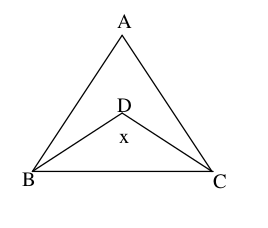
\includegraphics[scale=0.7]{figuras/fig28}
				\end{center}
				\begin{multicols}{5}
				\begin{enumerate}
					\item 120$^o$
					\item 130$^o$
					\item 150$^o$
					\item 100$^o$
					\item 40$^o$
				\end{enumerate}
				\end{multicols}
				
			\item Determine o valor dos termos desconhecidos nos triângulos abaixo:\\
			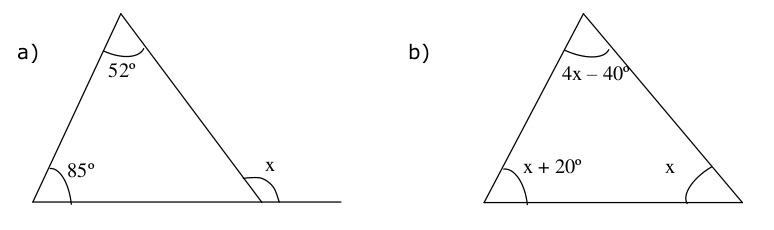
\includegraphics[scale=0.7]{figuras/fig26.png}\\
			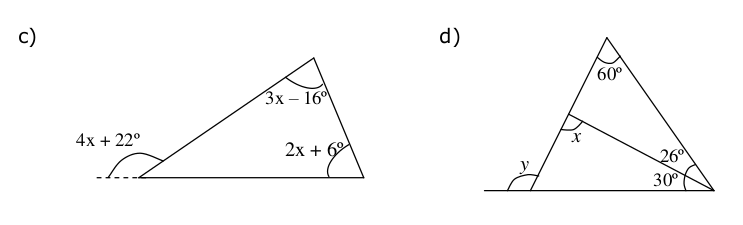
\includegraphics[scale=0.7]{figuras/fig27.png}
			
			\item Na figura, o $\bigtriangleup ABC$ é congruente ao $\bigtriangleup EDC$. Determine o caso de congruência e o valor de x e y.
			
			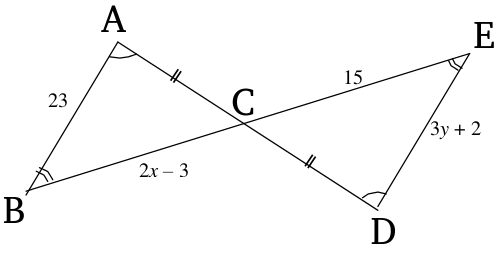
\includegraphics[scale=0.7]{figuras/fig29.png}
		\end{list}
		 \section{Congruência de Triângulo}	
		 	\begin{list}{\textbf{Questão \arabic{quest}.}}{\usecounter{quest}}
%define a margem da lista.	
%\setlength{\labelwidth}{-2mm} \setlength{\parsep}{0mm}
%\setlength{\topsep}{0mm} \setlength{\leftmargin}{-2mm}
\renewcommand{\labelenumi}{(\alph{enumi})}

		 		\item Os triângulos ABC e MNP são congruentes. Pelas indicações, determine o caso de congruências e as medidas x e y.	 		
		 		\begin{center}
		 		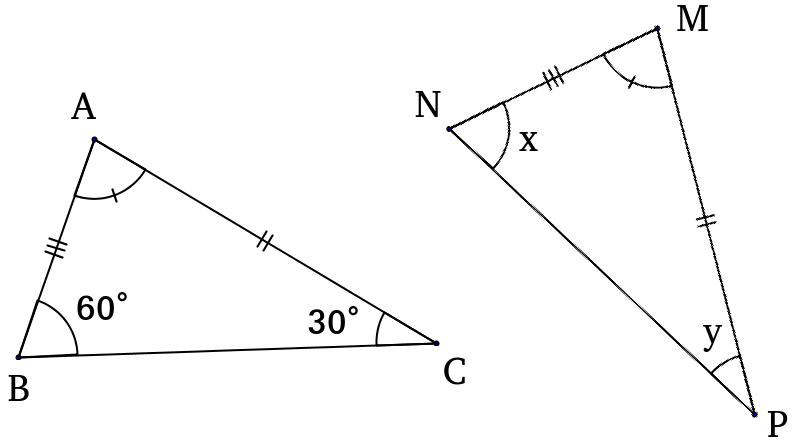
\includegraphics[scale=0.4]{figuras/fig17.png}
		 		\end{center}
		 		
		 		\item Na figura, $\widehat{B} \cong \widehat{E}$ e $\overline{AB} \cong \overline{DE}$. Nessas condições, determine as medidas de $x$ e $y$.		 		
		 		\begin{center}
		 		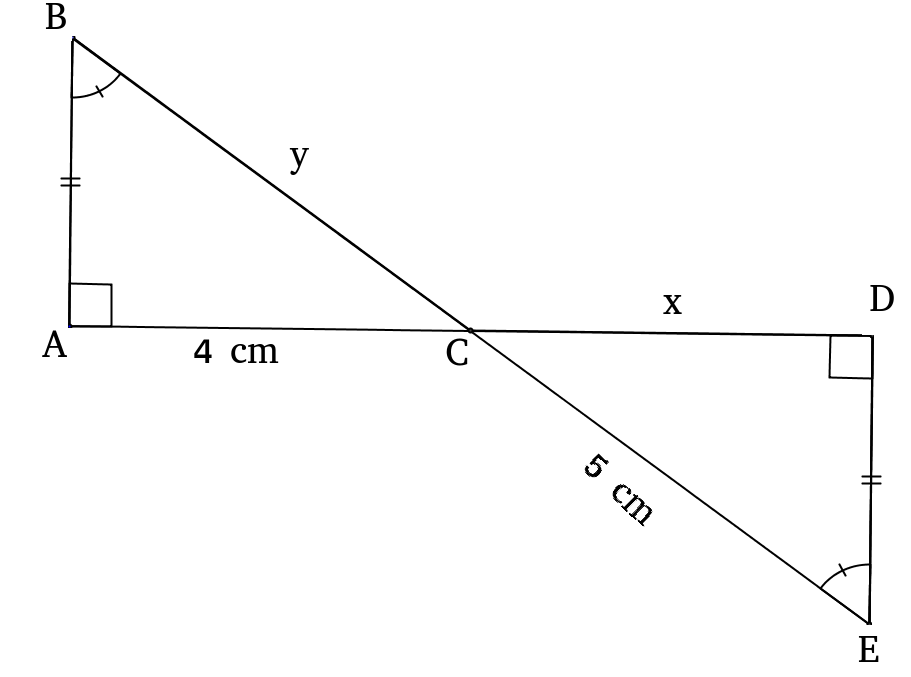
\includegraphics[scale=0.4]{figuras/fig18.png}
		 		\end{center}
		 		
		 		\item Na figura, prove que $\bigtriangleup ABC \cong \bigtriangleup CBD.$
		 		\begin{center}
		 		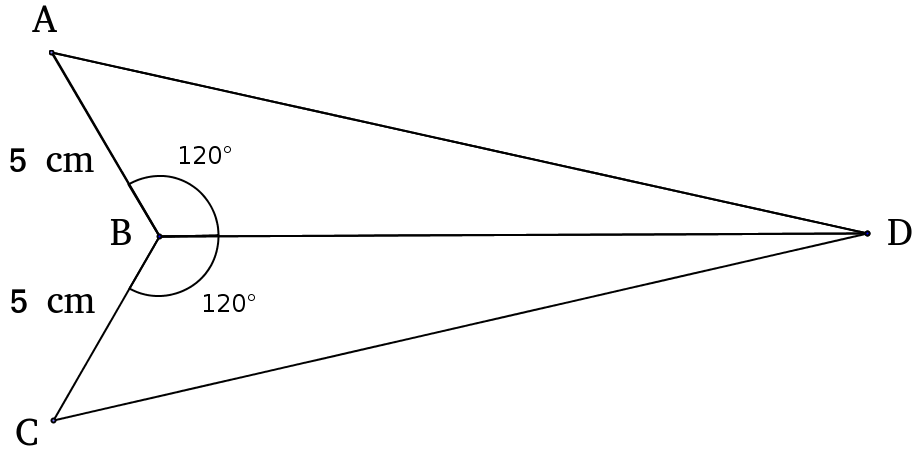
\includegraphics[scale=0.4]{figuras/fig19.png} 
		 		\end{center}
		 		
		 		\item Na figura, $\overline{AC} \cong \overline{MN}$ e $\widehat{C} \cong \widehat{N}$. Prove que $\overline{AB} \cong \overline{PM}$.
		 		\begin{center}
		 		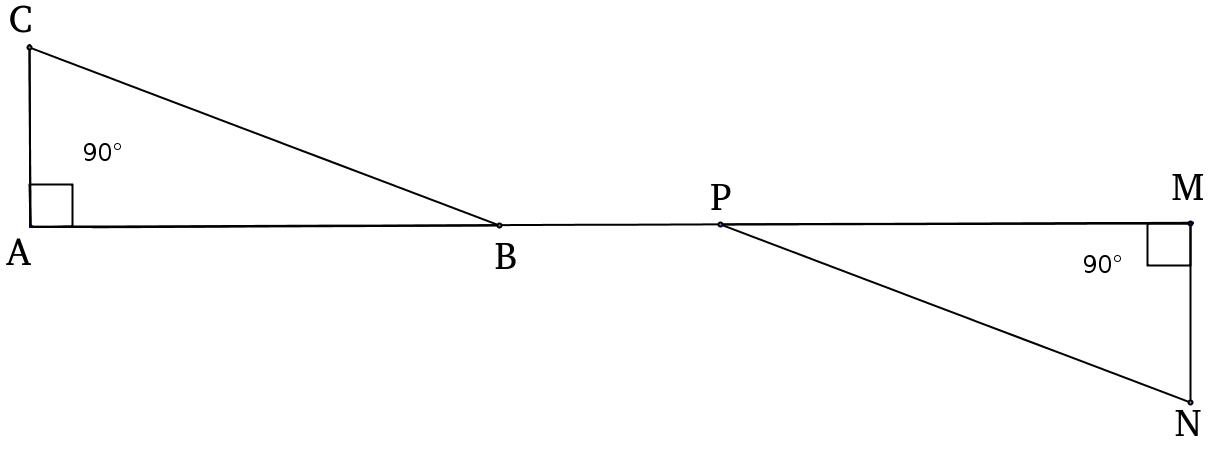
\includegraphics[scale=0.4]{figuras/fig20.png}
		 		\end{center}
		 		
		 		\item No $\bigtriangleup ABC, \overline{AB} \cong \overline{AC}$ e $\overline{BD} \cong \overline{DC}$. Nessas condições, mostre que:
		 		\begin{multicols}{3}
		 		\begin{enumerate}
		 			\item $x=y$.
		 			\item $\widehat{B} \cong \widehat{C}$.
		 			\item $\overline{AB}$ é altura do $\bigtriangleup ABC$.
		 		\end{enumerate}
		 		\end{multicols}
		 		
		 		\item (Saresp) Na figura, o triângulo ABC é isóceles e $\overline{BD} \cong \overline{DE} \cong \overline{EC}$. Nessas condições, os triângulos:
		 		\begin{enumerate}
		 			\item ABD e ADE são congruentes.
		 			\item ABD e AEC são congruentes.
		 			\item ADE e AEC são congruentes.
		 			\item ABD e ABC são congruentes.
		 		\end{enumerate}
		 		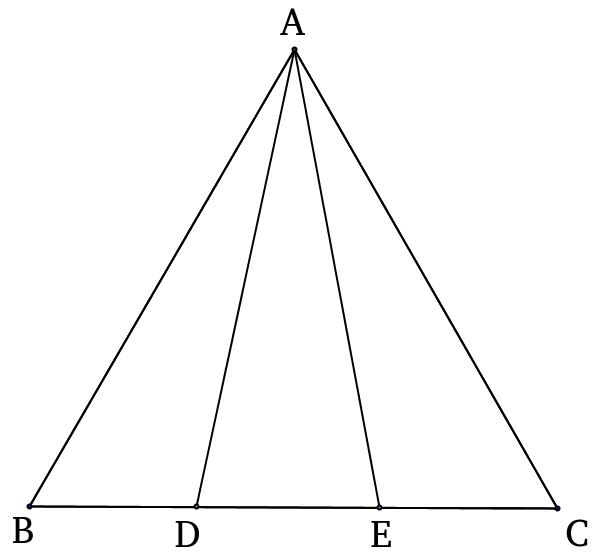
\includegraphics[scale=0.4]{figuras/fig21.png}
				
				\item Na figura, $\widehat{A} \cong \widehat{B}$ e $\overline{AM} \cong \overline{MB}$. Prove que $M$ é ponto médio de $\overline{CD}$.
				\begin{flushleft}
				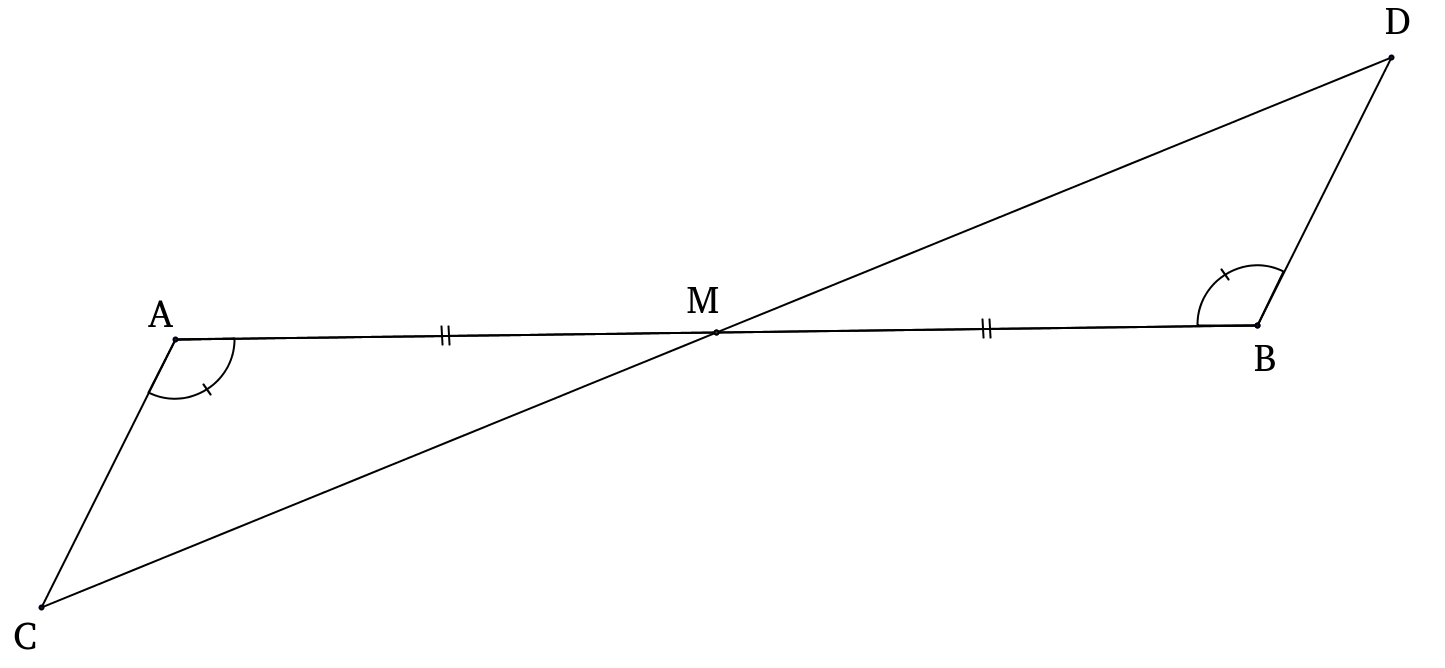
\includegraphics[scale=0.4]{figuras/fig22.png}
				\end{flushleft}
			\end{list}	
			
			\section{Quadriláteros}
			\begin{list}{\textbf{Questão \arabic{quest}.}}{\usecounter{quest}}
%define a margem da lista.	
%\setlength{\labelwidth}{-2mm} \setlength{\parsep}{0mm}
%\setlength{\topsep}{0mm} \setlength{\leftmargin}{-2mm}
\renewcommand{\labelenumi}{(\alph{enumi})}

				\item  Coloque (V) para verdadeiro e (F) para falso nas afirmativas abaixo:
				\begin{enumerate}
				\item ( \ ) As diagonais de um quadrado são sempre congruentes.
				\item ( \ ) As diagonais de um losango são sempre congruentes.
				\item ( \ ) As diagonais de um retângulo são sempre congruentes.
				\item ( \ ) As diagonais de um losango são sempre perpendiculares.
				\item ( \ ) Todo retângulo é um quadrado.
				\end{enumerate}
				
				\item Observe os paralelogramos e, considerando as propriedades estudadas, determine:
				\begin{multicols}{2}
				\begin{enumerate}
					\item MN e NP 
					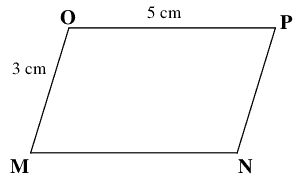
\includegraphics[scale=0.7]{figuras/fig30.png}
					\item x e y 
					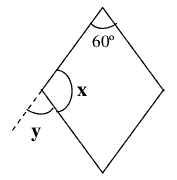
\includegraphics[scale=0.7]{figuras/fig31.png}
					\item $med(\widehat{A}),med(\widehat{B}),med(\widehat{C})$\\
					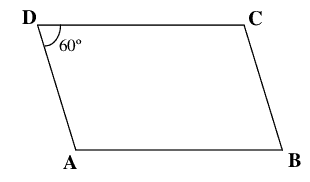
\includegraphics[scale=0.7]{figuras/fig32.png}
					\item O perímetro do triângulo RMS.
					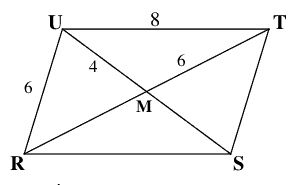
\includegraphics[scale=0.7]{figuras/fig33.png}
				\end{enumerate}
				\end{multicols}
				
				\item No retângulo ABCD da figura a seguir, M é ponto médio do lado CD. O valor da medida x indicada na figura abaixo é:
				\begin{center}
				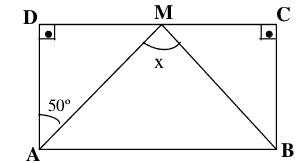
\includegraphics[scale=0.7]{figuras/fig34.png}
				\end{center}
				\begin{multicols}{5}
				\begin{enumerate}
					\item 50$^o$
					\item 45$^o$
					\item 100$^o$
					\item 75$^o$
					\item 80$^o$
				\end{enumerate}
				\end{multicols}
				
				\item Encontre os valores de x e y.
				\begin{multicols}{2}
				\begin{enumerate}
					\item ABCD é um losango
					\item[] 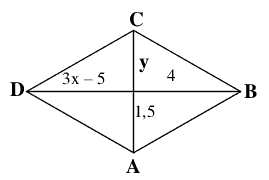
\includegraphics[scale=0.7]{figuras/fig35}
					\item ABCD é retângulo
					\item[] 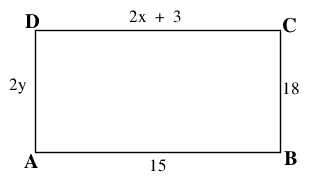
\includegraphics[scale=0.7]{figuras/fig36}
				\end{enumerate}
				\end{multicols}
				
				\item Observe o paralelogramo e determine:
				\begin{center}
				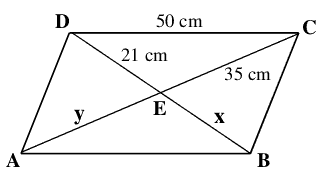
\includegraphics[scale=0.7]{figuras/fig37}
				\end{center}
				\begin{multicols}{2}
				\begin{enumerate}
					\item as medidas de x e Y indicadas.
					\item o perímetro do $\bigtriangleup ABC$
				\end{enumerate}
				\end{multicols}
				
				\item Calcula o valor de x e y nos trapézios abaixo.
				\begin{multicols}{2}
				\begin{enumerate}
					\item 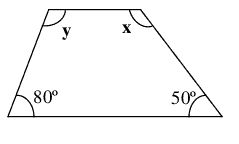
\includegraphics[scale=0.7]{figuras/fig38}
					\item 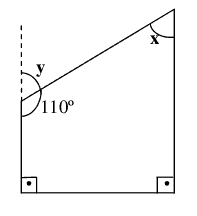
\includegraphics[scale=0.7]{figuras/fig39}
				\end{enumerate}
				\end{multicols}
				
				\item A figura abaixo é um trapézio isósceles. Sabendo que AM está contido na bissetriz do ângulo $\widehat{A}$ e BM está contido na bissetriz do ângulo $\widehat{B}$, o valor da medida x indicada é:
				\begin{center}
				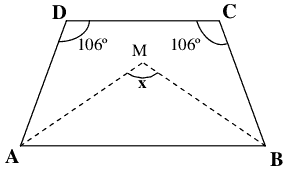
\includegraphics[scale=0.7]{figuras/fig40}
				\end{center}
				
				\begin{multicols}{4}
				\begin{enumerate}
					\item 74
					\item 36
					\item 104
					\item 106
				\end{enumerate}
				\end{multicols}
				
				\item No paralelogramo, temos: $med(\widehat{B}) = 80^o$, $\overline{BM}$ é bissetriz do $\widehat{A}$. Calcule a medida do ângulo $A\widehat{M}B$.
				
				\begin{center}
				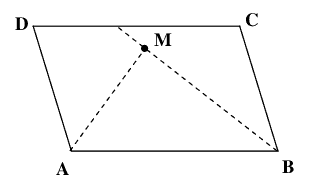
\includegraphics[scale=0.7]{figuras/fig41}
				\end{center}
			\end{list}


	\chapter{Conjuntos Numéricos}
\section{Atividade Elementares}
	\begin{list}{\textbf{Questão \arabic{quest}.}}{\usecounter{quest}}
%define a margem da lista.	
%\setlength{\labelwidth}{-2mm} \setlength{\parsep}{0mm}
%\setlength{\topsep}{0mm} \setlength{\leftmargin}{-2mm}
\renewcommand{\labelenumi}{(\alph{enumi})}

	\item Seja $A = \{ 1, \{2\}, \{1,2\} \}$. Considere as afirmações:
		\begin{multicols}{4}
		\newcounter{Romanos}
		\begin{list}{\Roman{Romanos} -}{\usecounter{Romanos}}
			\item $1 \displaystyle \in A$
			\item $2 \displaystyle \in A$
			\item $\displaystyle \varnothing \subset A$
			\item $\{1,2\} \displaystyle \subset A$
		\end{list}
		\end{multicols}
		Estão corretas as afirmações:
		\begin{multicols}{5}
		\begin{enumerate}
			\item I e II
			\item I e III
			\item III e IV	
			\item III
			\item I
		\end{enumerate}
		\end{multicols}

		\item Sabendo que A = {1, 2, 3, 4}, B = {4, 5, 6} e C = {1, 6, 7, 8, 9}, podemos afirmar que o conjunto $(A \displaystyle \cap B) \displaystyle \cup C$ é:
		\begin{multicols}{4}
		\begin{enumerate}
			\item \{1, 4\}
			\item \{1, 4, 6, 7\}
			\item \{1, 4, 5, 6\}	
			\item \{1, 4, 6, 7, 8, 9\}			
		\end{enumerate}
		\end{multicols}

		\item José Carlos e Marlene são os pais de Valéria. A família quer viajar nas férias de julho. José Carlos conseguiu tirar suas férias na fábrica do dia 2 ao dia 28. Marlene obteve licença no escritório de 5 a 30. As férias de Valéria na escola vão de 1 a 25. Durante quantos dias a família poderá viajar sem faltar as suas obrigações?
		\begin{multicols}{4}
		\begin{enumerate}
			\item 19
			\item 20
			\item 21 	
			\item  22			
		\end{enumerate}
		\end{multicols}

		\item (UNESP) Numa classe de 30 alunos, 16 gostam de Matemática e 20 gostam de História. O número de alunos desta classe que gostam de Matemática e História é:
		\begin{multicols}{3}
		\begin{enumerate}
			\item exatamente 16
			\item exatamente 10
			\item no máximo 6	
			\item no mínimo 6
			\item exatamente 18
		\end{enumerate}
		\end{multicols}

		\item (PUC) Numa pesquisa de mercado, verificou-se que 15 pessoas utilizam pelo menos um dos produtos A ou B. Sabendo que 10 destas pessoas não usam o produto B e que 2 destas pessoas não usam o produto A, qual é o número de pessoas que utilizam os produtos A e B?
		\begin{multicols}{4}
		\begin{enumerate}
			\item 2
			\item 3
			\item 4	
			\item 5 
		\end{enumerate}
		\end{multicols}
%===================================================================================================
	\item Qual é o conjunto dos números pares maiores que 50 e menores que 200?

	\item Qual é o conjunto das consoantes da palavra coco?

	\item Quantos elementos possui o conjunto \{3, 33, 333, 3333\}?

	\item Qual é o conjunto formado pelos números pares do número 31657?

	\item Faça um diagrama que satisfaça as seguintes condições: $2\in A, 4\notin A, 3\in A\cap B, A\cup B =\{2, 3, 4\}$.

	\item Como é representado um conjunto vazio?

	\item Seja o conjunto A = \{3, 4, 5, 6, 7, 8, 9\}, determine 3 subconjuntos de A, ou seja, 3 conjuntos que estejam contidos em A.

	\item Sabendo que A = \{0, 1, 2, ..., 98, 99\}, B = \{1, 2, 10, 12\} e C = \{10, 11, 12, ..., 98, 99\}, podemos afirmar que:
	\begin{enumerate}
	\begin{multicols}{4}
		\item $A\subset B$
		\item $B\subset C$
		\item $C\subset A$
		\item $A\subset C$
	\end{multicols}
	\end{enumerate}



	\item Sendo A = \{1, 2, 3, 4, 5\}, B = \{3, 4, 5, 6, 7\} e C = \{5, 6, 7, 8, 9\}, determine:
	\begin{enumerate}
	\begin{multicols}{4}
		\item $A\cup B$
		\item $A\cup C$
		\item $B\cup C$
		\item $A\cup B\cup C$
		\item $A\cap B$
		\item $A\cap C$	
		\item $B\cap C$
		\item $A\cap B\cap C$
	\end{multicols}
	\end{enumerate}
	
	\item Faça um diagrama que represente os conjuntos A, B e C da questão anterior.

	\item Quando temos $A\cap B = \varnothing$, dizemos que A e B são disjuntos. Escreva dois conjuntos, A e B, de modo que sejam disjuntos.

	\item Se o conjunto A tem 7 elementos, o conjunto B, 4 elementos e $A\cap B$ tem 1 elemento, quantos elementos terá $A\cup B$?

	\item Numa pesquisa em que foram ouvidas crianças, constatou-se que:
	\begin{itemize}
		\item 15 crianças gostavam de refrigerante.
		\item 25 crianças gostavam de sorvete
		\item 5 crianças gostavam de refrigerante e de sorvete
	\end{itemize}
	
Quantas crianças foram pesquisadas?

	\item Foram instaladas 66 lâmpadas para iluminar as ruas A e B, que se cruzam. Na rua A foram colocadas 40 lâmpadas e na rua B 30 lâmpadas. Quantas lâmpadas foram instaladas no cruzamento?

	\item Numa concentração de atletas há 42 que jogam basquetebol, 28 voleibol e 18 voleibol e basquetebol, simultaneamente. Qual é o número de atletas na concentração?

	\item Uma atividade com duas questões foi aplicada em uma classe de 40 alunos. Os resultados apontaram que 20 alunos haviam acertado as duas questões, 35 acertaram a primeira questão e 25, a segunda. Faça o diagrama e calcule o percentual de alunos que acertou apenas uma questão?

	\item Uma pesquisa de mercado foi realizada para verificar a audiência de três programas de televisão, 1200 famílias foram entrevistadas e os resultados obtidos foram os seguintes: 370 famílias assistem ao programa A, 300 ao programa B e 360 ao programa C. Desse total, 100 famílias assistem aos programas A e B, 60 aos programas B e C, 30 aos programas A e C e 20 famílias aos 3 programas.Com base nesses dados, determine:
	\begin{enumerate}
	\item quantas famílias não assistem a nenhum dos 3 programas?
	\item quantas famílias assistem ao programa A e não assistem ao programa C?
	\item qual o programa de maior fidelidade, ou seja, cujos espectadores assistem somente a esse programa?
	\end{enumerate}
	
	\end{list}
	\chapter{Função Afim}
		 \section{Atividades Básicas}	
		 	\begin{list}{\textbf{Questão \arabic{quest}.}}{\usecounter{quest}}
%define a margem da lista.	
%\setlength{\labelwidth}{-2mm} \setlength{\parsep}{0mm}
%\setlength{\topsep}{0mm} \setlength{\leftmargin}{-2mm}
\renewcommand{\labelenumi}{(\alph{enumi})}

		 	\item Seja a $f:\mathbb{R}\longrightarrow \mathbb{R}$ definida por $f(x)=4x+1$. Determine:
		 	\begin{multicols}{2}
		 	\begin{enumerate}
		 		\item $f(4)$
		 		\item $f(-2)$
		 		\item $f(-1)+f(0)-f(11)$
		 		\item $2f(3) - f(-3)$
		 	\end{enumerate}
		 	\end{multicols}
		 	
		 	\item Obtenha o domíno de cada função.
		 	\begin{multicols}{2}
		 	\begin{enumerate}
		 		\item $f(x)=9x+3$
		 		\item $g(x)=\displaystyle\frac{x^3 + 8x}{x+3}$
		 		\item $i(x) = \sqrt{x-8}$
		 		\item $j(x)=\displaystyle\frac{\sqrt{x-1}}{x-3}$
		 	\end{enumerate}
		 	\end{multicols}
		 	
		 	\item Dada à função do 1º grau $f(x) = (1 - 5x)$. Determinar:
		 	\begin{multicols}{4}
		 	\begin{enumerate}
		 		\item $f(0)$
		 		\item$f(-1)$
		 		\item $f(1/5)$
		 		\item $f(-1/5)$
		 	\end{enumerate}
			\end{multicols}		 	
		 				
			\item Considere a Função do 1º Grau $f(x) = -3x + 2$. Determine os valores de $x$ para que se tenha:
			\begin{multicols}{3}
			\begin{enumerate}
				\item $f(x) = 0$
				\item $f(x) = 11$
				\item $f(x) = -1/2$
			\end{enumerate}
			\end{multicols}
			
			\item Dada a função $f(x) = (ax + 2)$, determine o valor de a para que se tenha $f(4) = 22$.
			\item Dada a função $f(x) = ax + b$ e sabendo-se que $f(3) = 5$ e $f(-2) = -5$ calcule $f(1/2)$.
			\item Um vendedor recebe mensalmente um salário composto de duas partes: uma parte fixa, no valor de \$ 1.000,00 e uma parte variável que corresponde a uma comissão de 18\% do total de vendas que ele fez durante o mês.
				\begin{enumerate}
					\item Expressar a função que representa seu salário mensal.
					\item Calcular o salário do vendedor durante um mês, sabendo-se que vendeu \$ 10.000,00 em produtos.
				\end{enumerate}. 
			\item Em uma determinada loja, o salário mensal fixo de um vendedor é de R\$ 240,00. Além disso, ele recebe R\$ 12,00 por unidade vendida.
		\begin{enumerate}
			\item Expresse o ganho mensal (S) desse vendedor em função do número (u) de unidades vendidas.
			\item Quantas unidades ele deve vender para receber um salário de R\$ 700,00?
			\item Determine o domínio e a imagem desta função
		\end{enumerate}
		
		\item Um comerciante teve uma despesa de \$ 230,00 na compra de certa mercadoria. Como vai vender cada unidade por \$ 5,00, o lucro final L será dado em função das x unidades vendidas. Responda:
		\begin{enumerate}
		 	\item Qual a lei dessa função f;
		 	\item Para que valores de x têm f(x) < 0? Como podemos interpretar esse caso?
		 	\item Para que valores de x haverá um lucro de \$ 315,00?
		 	\item Para que valores de x o lucro será maior que \$ 280,00?
		\end{enumerate}
		
%+==========================================================================================
	\item Sendo $f(x) = x - 3$ e $g(x) = -3x + 4$, determine: 
	\begin{multicols}{3}
	\begin{enumerate}
		\item $f(f(0))$
		\item $g(g(2))$
		\item $f(f(0)) + g(g(2))$
	\end{enumerate}
	\end{multicols}		
	\item Esboce o gráfico da função sobre os números reais $f(x)  = 2x + 3$. 	
	\item Determine o domínio $D$ da função:
	\begin{multicols}{3}	
	\begin{enumerate}
		\item $f(x)=10x+5$
		\item $f(x)=\displaystyle\frac{2}{x}$
		\item $f(x)=\displaystyle\frac{1}{x-3}$
		\item $f(x)=\sqrt{x}$
		\item $f(x)=\sqrt{x+3}$
		\item $f(x)=\displaystyle\frac{3}{\sqrt{x-2}}$
	\end{enumerate}
	\end{multicols}	
	
	\item Determine se cada um dos gráficos abaixo representa uma função:
	\begin{multicols}{2}
	\begin{enumerate}
		\item 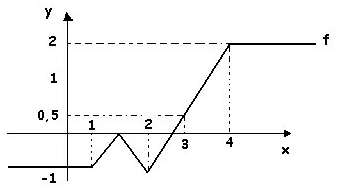
\includegraphics[scale=0.6]{figuras/fig10}
		\item 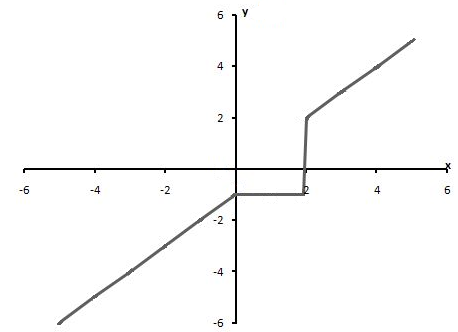
\includegraphics[scale=0.4]{figuras/fig11}
		\item \includegraphics[scale=0.9]{figuras/fig12}
		\item \includegraphics[scale=0.9]{figuras/fig13}			
	\end{enumerate}
	\end{multicols}	
	
	\item Na produção de peças, uma indústria tem um custo fixo de R\$ 8,00 mais um custo variável de R\$ 0,50 por unidade produzida. Sendo $x$ o número de unidades produzidas:
	\begin{enumerate}
		\item Escreva a lei da função que fornece o custo total de x peças;
		\item Calcule o custo de 100 peças;
		\item Escreva a taxa de crescimento da função.
	\end{enumerate}
	\item Na revelação de fotos, uma empresa calcula o preço a ser cobrado usando uma fórmula $P=12,00 + 0,65n$, onde $P$ é o preço, em reais, a ser cobrado e $n$ o número de fotos reveladas.
	\begin{enumerate}
		\item Quanto pagarei se forem reveladas 22 fotos?
		\item Se paguei a quantia de R\$ 33,45 pela revelação, qual o total de fotos reveladas?
	\end{enumerate}
		 		\item A cetesb detectou uma certa companhia jogando ácido sulfúrico no Rio Tiete, multou-a em \$ 125.000,00, mais \$ 1.000,00 por dia até que a companhia se ajustasse às normas legais que regulamentam os índices de poluição. Expresse o total de multa como função em numero de dias em que a companhia continuou violando as normas. 
		 		
		 		\item Em algumas cidades você pode alugar um carro \$ 154 por dia mais um adicional de \$ 16,00 por km. Determine a função por um dia e esboce no gráfico. Calcule o preço para se alugar por um dia e dirigi-lo por 200 km.
		 		
		 		\item Uma companhia de gás irá pagar para um proprietário de terra \$ 15.000,00 pelo direito de perfurar a terra para encontrar gás natural, e \$ 0,3 para cada mil pés cúbicos de gás
extraído. Expresse o total que o proprietário irá receber com função da quantidade de gás
extraído. Esboçar o gráfico.

				\item Em 1998, um paciente pagou \$ 300,00 por um dia em um quarto de hospital semiprivativo e \$ 1.500,00 por uma operação de apêndice. Expresse o total pago pela cirurgia como função do número de dias em que o paciente ficou internado.

				\item O preço a ser pago por uma corrida de táxi inclui uma parcela fixa, denominada bandeirada, e uma parcela que depende da distância percorrida. Se a bandeirada custa R\$ 5,50 e cada quilômetro rodado custa R\$ 0,90, calcule:

				\begin{enumerate}
					\item o preço de uma corrida de 10 km.
					\item a distância percorrida por um passageiro que pagou R\$ 19,00 pela corrida.	
				\end{enumerate}

16. As funções consumo e poupança de um operário de renda variável y são, respectivamente, $C = 100 + 0,6y$ e $S = 0,4y-100$.
				\begin{enumerate}
					\item Qual o seu consumo e sua poupança se ele ganhar R\$ 480,00?
					\item Qual o seu consumo se sua renda for nula? Como você explica a existência de consumo com uma renda nula?	
					\item Qual a sua poupança se sua renda for nula? Como você explica a existência de poupança negativa?
				\end{enumerate}

				\item Na revelação de um filme, uma ótica calcula o preço a ser cobrado usando a fórmula $P = 12,00 + 0,65n$, onde $P$ é o preço,em reais, a ser cobrado e $n$ o número de fotos reveladas do filme.
				\begin{enumerate}
					\item Quanto pagarei se forem reveladas 22 fotos do meu filme?
					\item Se paguei a quantia de R\$ 33,45 pela revelação, qual o total de fotos reveladas?
				\end{enumerate}


				\item O preço a ser pago por uma corrida de táxi inclui uma parcela fixa, denominada bandeirada, e uma parcela que depende da distância percorrida. Se a bandeirada custa R\$ 3,44 e cada quilômetro rodado custa R\$ 0,86, calcule:

				\begin{enumerate}
					\item o preço de uma corrida de 11 km;
					\item a distância percorrida por um passageiro que pagou R\$ 21,50 pela corrida.
				\end{enumerate}

				\item Um fabricante usa como política de vendas, colocar seu produto ao início de janeiro ao preço $p$ e aumentar mensalmente esse preço de 3,00. Em 1 de setembro esse preço passou a R\$ 54,00. Nestas condições determinar:
				\begin{enumerate}
					\item O preço inicial em janeiro
					\item Qual será o preço em dezembro
					\item Esboçar o gráfico da função que rege o preço do produto
				\end{enumerate}

		 	\end{list}	
		 	
	 	\section{Questões de Vestibular}
							
				\begin{center}
				\uppercase{Texto para próxima questão.}
				\end{center}
				Da  frieza  dos  números  da  pesquisa  saíram algumas recomendações. Transformadas em políticas públicas, poderiam reduzir a gravidade e as dimensões da tragédia urbana do trânsito. A   primeira é a adoção de práticas que possam reduzir a gravidade dos acidentes.A segunda     recomendação trata dos motociclistas, cuja frota equivale a 10\% do total, mas cujos custos   correspondem   a   19\%.O 'motoboy' ganha R\$2 por entrega, a empresa, R\$8. É um exército de garotos em disparada. O pedestre forma o contingente  mais vulnerável  no  trânsito  e  necessita  de  maior  proteção, diz a terceira recomendação da pesquisa. Entre a 0h e  as  18h  da  quinta-feira,  as  ambulâncias  vermelhas do  Resgate  recolheram  16  atropelados  nas  ruas  de São Paulo.
				
Fonte: "Folha de São Paulo", com adaptações
			\begin{list}{\textbf{Questão \arabic{quest}.}}{\usecounter{quest}}
%define a margem da lista.	
%\setlength{\labelwidth}{-2mm} \setlength{\parsep}{0mm}
%\setlength{\topsep}{0mm} \setlength{\leftmargin}{-2mm}
\renewcommand{\labelenumi}{(\alph{enumi})}

				\item  Conforme o texto, num dia de trabalho, são necessárias 12 entregas para um motoboy receber R\$24,00. Por medida de segurança, a empresa limitará a 10 a quantidade de entregas por dia. Como compensação, pagará um adicional fixo de p reais ao dia a quem atingir esse limite, porém reduzirá para R\$1,80 o valor pago por cada entrega. O valor de p que manterá inalterada a quantia diária recebida pelo motoboy, ou seja, R\$24,00, será:
				\begin{multicols}{5}				
				\begin{enumerate}
					\item R\$ 5,40
					\item R\$ 5,60
					\item R\$ 5,80
					\item R\$ 6,00
					\item R\$ 6,20
				\end{enumerate}
				\end{multicols}
				
				\begin{center}
				\uppercase{Texto para as próximas duas questões.}
				\end{center}
				(Faap) Medições realizadas mostram que a temperatura no interior da terra aumenta, 
aproximadamente, 3$^o$C a cada 100m de profundidade. Num certo local, a 100m de profundidade, a temperatura é de 25$^o$C. Nessas condições, podemos afirmar que:
				\item A temperatura a 1.500m de profundidade é:
				\begin{multicols}{5}
				\begin{enumerate}
					\item 70$^o$C
					\item 45$^o$C
					\item 42$^o$C
					\item 60$^o$C
					\item 67$^o$C
				\end{enumerate}
				\end{multicols}
				
				\item Encontrando-se uma fonte de água mineral a 46$^o$C, a profundidade dela será igual a:
				\begin{multicols}{5}
				\begin{enumerate}
					\item 700 m				
					\item 600 m
					\item 800 m
					\item 900 m
					\item 500 m
				\end{enumerate}								
				\end{multicols}
				
				\begin{center}
					\uppercase{texto para próxima questão.}
				\end{center}				
				(Enem) José Antônio viajarão em seus carros com as respectivas famílias para a cidade de Serra Branca. Com a intenção de seguir viagem juntos, combinam um encontro no marco inicial da rodovia, onde chegarão, de modo independente, ente meio-dia e 1 hora da tarde. Entretanto, como não querem ficar muito tempo esperando um pelo outro, combinam que o primeiro que chegar ao marco inicial esperará pelo outro, no máximo, meio hora; após esse tempo, seguirá viagem sozinho.		
				\item Chamando de $x$ o horário de chegada de José e de $y$ o horário de chegada de Antônio, e representando os pares (x; y) em um sistema de eixos cartesianos, a região OPQR a seguir indicada corresponde ao conjunto de todas as possibilidades para o par $(x, y)$:
				
				\begin{center}
				\includegraphics[scale=0.7]{figuras/fig24.png}
				\end{center}
				
				Na região indicada, o conjunto de pontos que representa o evento "José e Antônio chegam ao marco inicial exatamente no mesmo horário" corresponde:
				\begin{multicols}{4}
				\begin{enumerate}
					\item à diagonal OQ
					\item à diagonal PR
					\item ao lado PQ
					\item ao lado QR
					\item ao lado OR
				\end{enumerate}
				\end{multicols}
				
				\begin{center}
				\uppercase{texto para próxima questão.}
				\end{center}
				
				(Faap) A variação de temperatura $y=f(x)$ num intervalo
de tempo $x$ é dada pela função $f(x)=(m^2-9)x^2+(m+3)x+m-3$; calcule "m" de modo que:
				\item O gráfico da função seja uma reta e f(x) seja crescente:
				\begin{multicols}{5}
				\begin{enumerate}
					\item -3
					\item 9
					\item 3
					\item -9
					\item 0
				\end{enumerate}
				\end{multicols}
				
				\item (Mackenzie)
				
				\begin{center}
				\includegraphics[scale=0.7]{figuras/fig25.png}
				\end{center}
				
				Na figura temos os gráficos das funções $f$ e $g$. Se $f(x)=2x^2$, então $g(3)$ vale:
				\begin{multicols}{5}
				\begin{enumerate}
					\item 6
					\item 8
					\item 10
					\item 12
					\item 14
				\end{enumerate}
				\end{multicols}
				
				\item (Unesp) Considere a função $f:\mathbb{R} \longrightarrow \mathbb{R}$, definida por $f(x)=2x-1$. Determine todos os valores de $m \in \mathbb{R}$ para os quais é válida a igualdade: $$f(m^2)-2f(m)+f(2m)= \displaystyle\frac{m}{2}.$$
				
			    \item (Unesp) Um operário ganha R\$3,00 por hora de trabalho de sua jornada semanal regular de trabalho, que é de 40 horas. Eventuais horas extras são pagas com um acréscimo de 50\%. Encontre uma fórmula algébrica para expressar seu salário bruto semanal, $S$, para as semanas em que trabalhar h horas, com $h\geqslant40$.	
			    
			    \item (Unesp) Uma pessoa obesa, pesando num certo momento 156 kg, recolhe-se a um SPA onde se anunciam perdas de peso de até 2,5 kg por semana. Suponhamos que isso realmente ocorra. Nessas condições:
			    	\begin{enumerate}
			    		\item Encontre uma fórmula que expresse o peso mínimo, P, que essa pessoa poderá atingir após n semanas.
			    		\item Calcule o número mínimo de semanas completas que a pessoa deverá permanecer no SPA para sair de lá com menos de 120 kg de peso.
			    	\end{enumerate}
			
			\end{list}		 	
		\section{Atividades do Enem}				
			\begin{list}{\textbf{Questão \arabic{quest}.}}{\usecounter{quest}}
%define a margem da lista.	
%\setlength{\labelwidth}{-2mm} \setlength{\parsep}{0mm}
%\setlength{\topsep}{0mm} \setlength{\leftmargin}{-2mm}
\renewcommand{\labelenumi}{(\alph{enumi})}
	
				\item 06) (ENEM-08) Uma pesquisa da ONU estima que, já em 2008, pela primeira vez na história das civilizações,a maioria das pessoas viverá na zona urbana. O gráfico a seguir mostra o crescimento da população urbana desde 1950, quando essa população era de 700 milhões de pessoas, e apresenta uma previsão para 2030, baseada em crescimento linear no período de 2008 a 2030.			
				\begin{center}
				\includegraphics[scale=0.8]{figuras/fig14}
				\end{center}
	De acordo com o gráfico, a população urbana mundial em 2020 corresponderá, aproximadamente, a quantos bilhões de pessoas?
				\begin{multicols}{5}
				\begin{enumerate}
					\item 4,00
					\item 4,10
					\item 4,15
					\item 4,25 
					\item 4,50
				\end{enumerate}
				\end{multicols}
				
				\item (UNIRIO) O valor de um carro popular decresce linearmente com o tempo, devido ao desgaste. Sabendo-se que o preço de fábrica é R\$ 7.500,00 e que, depois de 6 anos de uso, é R\$ 1.200,00, seu valor após 4 anos de uso, em reais é:
				\begin{multicols}{4}
				\begin{enumerate}
					\item 2.100
					\item 2.400
					\item 3.150
					\item 3.300 					 
				\end{enumerate}
				\end{multicols}
				
				\item (UERJ) - Em uma partida, Vasco e Flamengo levaram ao Maracanã 90.000 torcedores. Três portões foram abertos às 12 horas e até as 15 horas entrou um número constante de pessoas por minuto. \newline A partir desse horário, abriram-se mais 3 portões e o fluxo constante
de pessoas aumentou. Os pontos que definem o número de pessoas dentro do estádio em função do horário de entrada estão contidos no gráfico abaixo:
				\begin{center}
				\includegraphics[scale=0.8]{figuras/fig15}
				\end{center}
				Quando o número de torcedores atingiu 45.000, o relógio estava marcando 15 horas e:
				\begin{multicols}{4}
				\begin{enumerate}
					\item 20 min
					\item 30 min
					\item 40 min
					\item 50 min 					 
				\end{enumerate}
				\end{multicols}
				
				\item Um helicóptero desloca-se numa trajetória cuja equação é $y=\displaystyle\frac{1}{2}x+100$. Um míssil disparado contra o helicóptero segue uma trajetória cuja
equação é $y = 2(x -10) + k$. Em ambas as equações,$y$ representa a altura em relação ao eixo $Ox$. O míssil atinge o helicóptero a uma altura de 130 m. Se as distâncias $x$ e $y$ são dadas em metros, o valor de $k$ será:
				\begin{multicols}{4}
				\begin{enumerate}
					\item 0
					\item 10
					\item 20
					\item 30 					 
				\end{enumerate}
				\end{multicols}


			\end{list}	


	\chapter{Teorema de Tales}
\begin{list}{\textbf{Questão \arabic{quest}.}}{\usecounter{quest}}
%define a margem da lista.	
%\setlength{\labelwidth}{-2mm} \setlength{\parsep}{0mm}
%\setlength{\topsep}{0mm} \setlength{\leftmargin}{-2mm}
\renewcommand{\labelenumi}{(\alph{enumi})}

	\item Nas figuras, a // b // c, calcule o valor de x.
		\begin{multicols}{2}
		\begin{enumerate}
			\item \includegraphics[scale=0.7]{figuras/fig46.png}
			\item \includegraphics[scale=0.7]{figuras/fig47.png}
			\item \includegraphics[scale=0.7]{figuras/fig48.png}
			\item \includegraphics[scale=0.7]{figuras/fig49.png}
			\item \includegraphics[scale=0.7]{figuras/fig50.png}
			\item \includegraphics[scale=0.7]{figuras/fig51.png}
			\item \includegraphics[scale=0.7]{figuras/fig52.png}
		\end{enumerate}
		\end{multicols}
		
	\item Determine x e y, sendo r, s, t e u retas paralelas.
		\begin{multicols}{2}
		\begin{enumerate}
			\item \includegraphics[scale=0.7]{figuras/fig53.png}
			\item \includegraphics[scale=0.7]{figuras/fig54.png}
			\item \includegraphics[scale=0.7]{figuras/fig55.png}
			\item \includegraphics[scale=0.7]{figuras/fig56.png} 
		\end{enumerate}
		\end{multicols}
		
	\item Determine x e y, sendo r, s e t retas  paralelas.
	\begin{center}
	\includegraphics[scale=0.7]{figuras/fig57.png}
	\end{center}
	
	\item Uma reta paralela ao lado $\overline{BC}$ de um triângulo ABC determina o ponto D em $\overline{AB}$ e E em $\overline{AC}$. Sabendo-se que $\overline{AD}= x$, $\overline{BD} = x + 6$,  $\overline{AE} = 3$ e $\overline{EC} = 4$, determine o lado $\overline{AB}$ do triângulo.
	
	\item A figura abaixo indica três lotes de terreno com frente para a rua A e para rua B. as divisas dos lotes são perpendiculares à rua A. As frentes dos lotes 1, 2 e 3 para a rua A, medem, respectivamente, 15 m, 20 m e 25 m. A frente do lote 2 para a rua B mede 28 m. Qual é a medida da frente para a rua B dos lotes 1 e 3?
	\begin{center}
	\includegraphics[scale=0.7]{figuras/fig58.png}
	\end{center}
	
	\item Um  feixe de quatro retas paralelas determina sobre uma transversal três segmentos consecutivos, que medem 5 cm, 6 cm e 9 cm. Calcule os comprimentos dos segmentos determinados pelo feixe em outra transversal, sabendo que o segmento desta, compreendido entre a primeira e a quarta paralela, mede 60 cm.
	
	\item As alturas de dois postes estão entre si assim como 3 esta para 5. Sabendo que o menor deles mede 6 m, então o maior mede:
	
	\item A figura abaixo nos mostra duas avenidas que partem de um mesmo ponto A e cortam duas ruas paralelas. Na primeira avenida, os quarteirões determinados pelas ruas paralelas tem 80 m e 90 m de comprimento, respectivamente. Na segunda avenida, um dos quarteirões determinados mede 60 m. Qual o comprimento do outro quarteirão?
	\begin{center}
	\includegraphics[scale=0.5]{figuras/fig59.png}
	\end{center}
	
	\item Na figura abaixo, sabe-se que $\overline{RS}//\overline{DE}$ e que $\overline{AE} = 42 cm$. Nessas condições, determine as medidas x  e y indicadas.
	\begin{center}
	\includegraphics[scale=0.5]{figuras/fig60.png}
	\end{center}
	
	\item Num triângulo ABC, o lado $\overline{AB}$ mede 24 cm. Por um ponto D, sobre o lado $\overline{AB}$, distante 10 cm do vértice A, traça-se a paralela ao lado $\overline{BC}$, que corta o lado $\overline{AC}$ no ponto E e $\overline{AE}$ tem 15 cm, determine a medida do lado $\overline{AC}$.
	
	\item No triângulo ABC da figura, sabe-se que $\overline{DE} // \overline{BC}$. Calcule as medidas dos lados $\overline{AB}$ e $\overline{AC}$ do triângulo.
	\begin{center}
	\includegraphics[scale=0.5]{figuras/fig61.png}
	\end{center}
	
	\item Na figura abaixo, $\overline{AE} // \overline{BD}$. Nessas condições, determine os valores de a e b.
	\begin{center}
	\includegraphics[scale=0.5]{figuras/fig62.png}
	\end{center}
	
	\item A planta abaixo no mostra três terrenos cujas laterais são paralelas. Calcule, em metros, as medidas x, y e z indicadas.
	\begin{center}
	\includegraphics[scale=0.5]{figuras/fig63.png}
	\end{center}
	
	\item Dois postes perpendiculares ao solo estão a uma distância de 4 m um do outro, e um fio bem esticado de 5 m liga seus topos, como mostra a figura abaixo. Prolongando esse fio até prende-lo no solo, são utilizados mais 4 m de fio. Determine a distância entre o ponto onde o fio foi preso ao solo e o poste mais próximo a ele.
	\begin{center}
	\includegraphics[scale=0.5]{figuras/fig64.png}
	\end{center}
	
	\item No triângulo abaixo, sabe-se que $\overline{DE} // \overline{BC}$. Calcule as medidas dos lados  $\overline{AB}$ e $\overline{AC}$ do triângulo.
	\begin{center}
	\includegraphics[scale=0.7]{figuras/fig65.png}
	\end{center}
	
	\item Em um triângulo retângulo, a hipotenusa mede 14 cm e um dos catetos mede $5\sqrt{3}$cm. Determine a medida do outro cateto.
\end{list}	
	\chapter{Teorema de Pitágoras}
\begin{list}{\textbf{Questão \arabic{quest}.}}{\usecounter{quest}}
%define a margem da lista.	
%\setlength{\labelwidth}{-2mm} \setlength{\parsep}{0mm}
%\setlength{\topsep}{0mm} \setlength{\leftmargin}{-2mm}
\renewcommand{\labelenumi}{(\alph{enumi})}

\item Aplicando o teorema de Pitágoras, determine a medida x indicada em cada um dos triângulos retângulos.
	\begin{multicols}{2}
	\begin{enumerate}
		\item \includegraphics[scale=0.5]{figuras/fig68.png}
		\item \includegraphics[scale=0.5]{figuras/fig69.png}
		\item \includegraphics[scale=0.5]{figuras/fig70.png}
		\item \includegraphics[scale=0.5]{figuras/fig71.png}
		\item \includegraphics[scale=0.5]{figuras/fig72.png}
		\item \includegraphics[scale=0.5]{figuras/fig72.png}
		\item \includegraphics[scale=0.5]{figuras/fig73.png}		
	\end{enumerate}
	\end{multicols}
	
	\item Os lados de um triângulo ABC medem 10cm, 24cm e 26cm. Você pode afirmar que esse triângulo é retângulo?


	\item Em um triângulo retângulo, a hipotenusa mede 14cm e um dos catetos mede $5\sqrt{3}$ cm. Determine a medida do outro cateto.

	\item As medidas dos catetos de um triângulo retângulo medem $(2+\sqrt{5})$ cm e $(-2+\sqrt{5})$ cm. Determine a medida da hipotenusa.

	\item Um terreno triangular tem frentes de 12m e 16m em duas ruas que formam um ângulo de 90º. Quanto mede o terceiro lado desse terreno?

	\item O portão de entrada de uma casa tem 4m de comprimento e 3m de altura. Que comprimento teria uma trave de madeira que se estendesse do ponto A até o ponto C?
\begin{center}
		\includegraphics[scale=0.5]{figuras/fig74.png}

	\end{center}	
	\item Dois navios partem de um mesmo ponto, no mesmo instante, e viajam com velocidades constante em direções que formam um ângulo reto. Depois de uma hora de viagem, a distância entre os dois navios é 13 milhas. Se um deles é 7 milhas por hora mais rápido que o outro, determine a velocidade de cada navio.
\begin{center}
		\includegraphics[scale=0.5]{figuras/fig75.png}

	\end{center}	
	\item Durante um incêndio num edifício de apartamentos, os bombeiros utilizaram uma escada Magirus de 10 m para atingir a janela do apartamento sinistrado. A escada estava colocada a 1m do chão, sobre um caminhão que se encontrava afastado 6m do edifício. Qual é a altura do apartamento sinistrado em relação ao chão?
\begin{center}
		\includegraphics[scale=0.5]{figuras/fig76.png}

	\end{center}	
	\item Quantos metros de fio são necessários para "puxar luz" de um poste de 6m de altura até a caixa de luz que está ao lado da casa e a 8m da base do poste?
\begin{center}
		\includegraphics[scale=0.5]{figuras/fig77.png}

	\end{center}	
	\item Na figura, o triângulo BCD é equilátero.
\begin{center}
	\includegraphics[scale=0.5]{figuras/fig78.png}

\end{center}
Determine:
	\begin{enumerate}
	\item o perímetro do triângulo BCD.
	\item o perímetro do quadrilátero ABCD
	\end{enumerate}
	\item Na figura tem-se que $\overline{AB} \cong \overline{BC}$ e F é o ponto médio do lado $\overline{BE}$ do retângulo BCDE. 
	Determine 
\begin{center}
		\includegraphics[scale=0.5]{figuras/fig79.png}	

	\end{center}	\begin{enumerate}
	\item a medida x indicada na figura.
	\item a área do retângulo BCDE.		
	\end{enumerate}
	
\end{list}
	%Data da última alteração:19/10/2016
\chapter{Trigonometria}
\begin{list}{\textbf{Questão \arabic{quest}.}}{\usecounter{quest}}
%define a margem da lista.	
%\setlength{\labelwidth}{-2mm} \setlength{\parsep}{0mm}
%\setlength{\topsep}{0mm} \setlength{\leftmargin}{-2mm}
\renewcommand{\labelenumi}{(\alph{enumi})}

\item Determine no triângulo retângulo ABC da figura o valor do seno, do cosseno e da tangente do ângulo agudo $\beta$. Considere $\sqrt{3}=3$
\begin{center}
\includegraphics[scale=0.8]{figuras/fig84.png}
\end{center}

\item No triângulo retângulo da figura temos $tg\ \alpha=\displaystyle\frac{2}{3}$. Nessas condições, determine as medidas $x$ e $y$ indicadas.
\begin{center}
\includegraphics[scale=0.8]{figuras/fig85.png}
\end{center}

\item Determine a medida de x do cateto $AC$, no triângulo retângulo da figura. (Use: $sen\ 28º 
= 0,46$; $cos\ 28º = 0,88$ e $tg\ 28º = 0,53$)
\begin{center}
\includegraphics[scale=0.8]{figuras/fig86.png}
\end{center}


\item Encontre o valor do seno, cosseno e tangente do ângulo $\alpha$ nos triângulos retângulos a seguir.
\begin{multicols}{2}
\begin{enumerate}
	\item \includegraphics[scale=0.7]{figuras/fig87.png}
	\item \includegraphics[scale=0.7]{figuras/fig88.png}
	\item \includegraphics[scale=0.7]{figuras/fig89.png}
	\item \includegraphics[scale=0.7]{figuras/fig90.png}
\end{enumerate}
\end{multicols}

\item Um garoto, curioso para saber a altura do prédio de um shopping, conseguiu com seu professor de Matemática um teodolito (tipo de instrumento de medição de ângulos) para auxiliá-lo nesse desafio. A situação é representada pela figura a seguir.
\begin{center}
\includegraphics[scale=0.2]{figuras/fig91.png}
\end{center}
Suponha que a altura dos olhos do garoto com relação ao chão é de 1,50 m e que sua distância ao prédio do shopping é de 45 m. Sendo $tg\ \alpha = 2$, qual a altura do prédio?

\item Três amigos gostam de empinar pipa. Certo dia, com a pipa no ar, eles desenrolaram todo o carretel de linha, de 30 metros, conforme o desenho seguir.
\begin{center}
\includegraphics[scale=0.2]{figuras/fig92.png}
\end{center}
Sabendo que o seno do ângulo de inclinação da linha em relação ao solo é igual a 0,4, qual a altura aproximada da pipa?

\item Ao ancorar seu barco no Litoral Norte do estado de São Paulo, um pescador pode observar duas ilhas,A e B, como mostra a ilustração.
\begin{center}
\includegraphics[scale=0.3]{figuras/fig93.png}
\end{center}
Qual a distância do barco do pescador em relação à ilha B? (use $cos\ \alpha = 0,8$).

\item Utilizando o seno dos ângulos indicados, encontre o valor de $x$.
\begin{multicols}{2}
\begin{enumerate}
	\item \includegraphics[scale=0.7]{figuras/fig94.png}
	\item \includegraphics[scale=0.7]{figuras/fig95.png}
	\item \includegraphics[scale=0.7]{figuras/fig96.png}
	\item \includegraphics[scale=0.7]{figuras/fig97.png}
	\item \includegraphics[scale=0.7]{figuras/fig98.png}
\end{enumerate}
\end{multicols}
\end{list}
	\chapter{Progressões Aritméticas}
	\section{Atividada a serem reorganizadas}
	\begin{list}{\textbf{Questão \arabic{quest}.}}{\usecounter{quest}}
%define a margem da lista.	
%\setlength{\labelwidth}{-2mm} \setlength{\parsep}{0mm}
%\setlength{\topsep}{0mm} \setlength{\leftmargin}{-2mm}
\renewcommand{\labelenumi}{(\alph{enumi})}

		\item Determine o 52º termo da PA ( 8, 14, 20, 26, ...) 
		\begin{multicols}{4}
		\begin{enumerate}
			\item 308
			\item 326
			\item 314
			\item 320
		\end{enumerate} 
		\end{multicols}

		\item Determine o 43 termo da PA (-30, -25, -20, -15, ...) 
		\begin{multicols}{4}
		\begin{enumerate}
			\item 240
			\item 180
			\item 200
			\item 195
		\end{enumerate} 
		\end{multicols}

		\item Encontre a razão da PA, tal que $a_{1} = 15$ e $a_{16} = 45$:
		 \begin{multicols}{4}
		\begin{enumerate}
			\item 1
			\item 0
			\item -1 
			\item 2 
		\end{enumerate} 
		\end{multicols}
		
		\item Encontre a razão da PA, tal que $a_{1} = -5$ e $a_{301} = 1195$: 
		\begin{multicols}{4}
		\begin{enumerate}
			\item 395
			\item 400
			\item 380 
			\item  250
		\end{enumerate} 
		\end{multicols}
		
		\item O primeiro termo de uma PA é 100 e o trigésimo é 187. Qual a soma dos trinta primeiros termos? 
		\begin{multicols}{4}
		\begin{enumerate}
			\item 287
			\item 5650
			\item 4305 
			\item 2355   
		\end{enumerate} 
		\end{multicols}
		
		\item Sabendo que o primeiro termo de uma PA vale 21 e a razão é 7, calcule a soma dos 12 primeiros termos desta PA: 
		\begin{multicols}{4}
		\begin{enumerate}
			\item 714
			\item 650
			\item 305 
			\item 355 
		\end{enumerate} 
		\end{multicols}
		
		\item O sétimo termo de uma PA é 20 e o décimo é 32. Então o vigésimo termo é 
		\begin{multicols}{4}
		\begin{enumerate}
			\item 60
			\item 59
			\item 72 
			\item 76 
		\end{enumerate} 
		\end{multicols}
		
		\item O número mensal de passagens de uma determinada empresa aérea aumentou no ano passado nas seguintes condições: em janeiro foram vendidas 33.000 passagens; em fevereiro, 34.500; em março, 36.000. Esse padrão de crescimento se mantém para os meses subsequentes. Quantas passagens foram vendidas por essa empresa em julho do ano passado?
		\begin{multicols}{5}
		\begin{enumerate}
			\item 38.000
			\item 40.500
			\item 41.000 
			\item 42.000
			\item 48.000 
		\end{enumerate} 
		\end{multicols}

		\item Numa PA em que $a_{1} = 2$ e $a_{20} = 10$ Qual é a soma dos 20 primeiros termos dessa PA?
		\begin{multicols}{5}
		\begin{enumerate}
			\item 420
			\item 240
			\item 300 
			\item 300 
			\item 120.
		\end{enumerate} 
		\end{multicols}

		\item Numa PA em que $a_{6} = 2$ e $a_{38} = 10$ Qual é a soma dos 20 primeiros termos dessa PA?
		\begin{multicols}{5}
		\begin{enumerate}
			\item 120/3
			\item 125/4
			\item 150/3 
			\item 125/2 
			\item 100.
		\end{enumerate} 
		\end{multicols}

		\item Qual é a soma dos 20 primeiros pares não negativos?
		\begin{multicols}{5}
		\begin{enumerate}
			\item 420
			\item 400
			\item 380 
			\item 300 
			\item 100.
		\end{enumerate} 
		\end{multicols}

		\item Qual é a soma dos 20 primeiros múltiplos positivos de 7?
		\begin{multicols}{5}
		\begin{enumerate}
			\item 7000
			\item 147
			\item 1407 
			\item 7007 
			\item 140.
		\end{enumerate} 
		\end{multicols}
		\end{list}

	\chapter{Progressões Geométricas.}
\begin{list}{\textbf{Questão \arabic{quest}.}}{\usecounter{quest}}
%define a margem da lista.	
%\setlength{\labelwidth}{-2mm} \setlength{\parsep}{0mm}
%\setlength{\topsep}{0mm} \setlength{\leftmargin}{-2mm}
\renewcommand{\labelenumi}{(\alph{enumi})}

\item A sequência seguinte é uma progressão geométrica, observe: (2, 6, 18, 54...). Determine o 8º termo dessa progressão

\item Um carro, cujo preço à vista é R\$ 24 000,00, pode ser adquirido dando-se uma entrada e o restante em 5 parcelas que se encontram em progressão geométrica. Um cliente que optou por esse plano, ao pagar a entrada, foi informado que a segunda parcela seria de R\$ 4 000,00 e a quarta parcela de R\$ 1 000,00. Quanto esse cliente pagou de entrada na aquisição desse carro?

\item Sabendo que uma PG tem $a_1 = 4$ e razão $q = 2$, determine a soma dos 10 primeiros termos dessa progressão. 

\item Calcule o quarto e o sétimo termos da P. G. $(3, -6, 12,...)$.

\item Determine o segundo termo de uma P. G. crescente tal que $a_1 = 8$ e $a_3 = 18$.

\item As medidas do lado, do perímetro e da área de um quadrado estão em progressão geométrica, nessa ordem. Qual é área do quadrado.

\item Determine, de modo que a sequência $(4, 4x , 10x +6)$ seja PG.

\item Determine o 15º termo da PG $(256,128,64,32,...)$

\item Determine o 10º termo da PG $(3,6,12...)$.

\item Determine a PG de três termos sabendo do que o produto desses termos é 8 a soma do 2º com o 3º termo é 10.

\end{list}
	\chapter{Análise Combinatória} \
		\section{Princípio Fundamental da contagem}
		\begin{list}{\textbf{Questão \arabic{quest}.}}{\usecounter{quest}}
%define a margem da lista.	
%\setlength{\labelwidth}{-2mm} \setlength{\parsep}{0mm}
%\setlength{\topsep}{0mm} \setlength{\leftmargin}{-2mm}
\renewcommand{\labelenumi}{(\alph{enumi})}

		
		\item Thiago possui 3 blusas diferentes e 2 calças diferentes. De quantas maneiras ele poderá escolher uma blusa e uma calça para se vestir?
		
		\item Quantos números de dois algarismos podem ser formados utilizando elementos do conjunto  {1, 2, 3}?
		
		\item Quantos números de dois algarismos diferentes (distintos) podem ser formados utilizando elementos do conjunto {1, 2, 3}?
		
		\item Quantos números de três algarismos podem ser formados utilizando elementos do conjunto {1, 2, 3}?

		\item Quantos números de três algarismos diferentes (distintos) podem ser formados utilizando elementos do conjunto {1, 2, 3}?

		\item Um estádio possui 4 portões. De quantas maneiras diferentes um torcedor pode entrar e sair desse estádio? 
		
		\item Um estádio possui 4 portões. De quantas maneiras diferentes um torcedor pode entrar e sair desse estádio utilizando, para sair, um portão diferente do que entrou? 
		
		\item Mariana desenhou uma bandeira retangular de 3 listras e deseja pintá-la, de modo que duas listras consecutivas não sejam pintadas da mesma cor. Se ela possui 4 lápis de cores diferentes, de quantas maneiras poderá pintar sua bandeira? 
		
		\item Numa prova havia 4 itens para que os alunos respondessem V (verdadeiro) ou F (falso). De quantas maneiras diferentes um aluno que vai “chutar” todas as repostas poderá responder esses itens? 
		
		\item Um painel luminoso retangular é composto por 5 lâmpadas. De quantas maneiras diferentes esse painel pode estar iluminado? (considera-se o painel iluminado se, pelo menos, uma de suas lâmpadas estiver acesa) 
		
		\item Quantos números de 3 algarismo distintos podem ser formados usando-se os algarismo 1,2,3,4 e 5?

		\item Um restaurante oferece no cardápio 2 saladas distintas,e 4 ti podes de pratos de carne,5 variedades de bebidas e 3 sobremesas diferentes. Uma pessoa deseja uma salada,um prato de carne,uma bebida e uma sobremesa.De quantas maneiras a pessoa poderá fazer seu pedido?
		
		\item Quatro times de futebol(Vasco,Atlético,Corinthians e Internacional ) disputam um torneio.Quantos e quais são as possibilidades de classificação para os três primeiros lugares?
		
		\item Numa eleição de uma escola há 3 candidatos a presidente,cinco a vice-presidente,à secretario e 7 a tesoureiro.Quantos podem ser os resultados da eleição?
		
		 \item Com os algarismos 1, 2, 3, 4, 5 e 6, quantos números de três algarismos distintos podemos formar?
		 \begin{multicols}{5}
		 \begin{enumerate}[a)]
		 	\item 30
		 	\item 60
		 	\item 90
		 	\item 120
		 	\item 150
		 \end{enumerate}
		 \end{multicols}

		\item Uma prova consta de 10 questões do tipo V ou F. De quantas maneiras distintas ela pode ser resolvida?
		\begin{multicols}{5}
		 \begin{enumerate}[a)]
		 	\item 128
		 	\item 256
		 	\item 512
		 	\item 1024
		 	\item 2048
		 \end{enumerate}
		 \end{multicols}

		\item Quantos números de três algarismos podemos com os algarismos 0, 1, 2, 3, 4, 5, 6 e 7?
		\begin{multicols}{5}
		 \begin{enumerate}[a)]
		 	\item 348
		 	\item 448
		 	\item 548
		 	\item 648
		 	\item 748
		 \end{enumerate}
		 \end{multicols}

		\item Quantos números ímpares de três algarismos distintos podemos formar com os algarismos 0, 1, 2, 3, 4, 5, 6 e 7?
		\begin{multicols}{5}
		 \begin{enumerate}[a)]
		 	\item 72
		 	\item 144
			\item 200
			\item 240
			\item 288
		 \end{enumerate}
		 \end{multicols}

		\item Um jantar constará de três partes: entrada, prato principal e sobremesa. De quantas maneiras distintas ele poderá ser composto, se há como opções oito entradas, cinco pratos principais e quatro sobremesa?
		\begin{multicols}{5}
		 \begin{enumerate}[a)]
		 	\item 160
		 	\item 150
		 	\item 120
		 	\item 80 
		 	\item 17 
		 \end{enumerate}
		 \end{multicols}
		 
		 \item Se um quarto tem 5 portas, o número de maneiras distintas de se entrar nele e sair dele por um porta diferente é:
		\begin{multicols}{5}
		 \begin{enumerate}[a)]
		 	\item 5
		 	\item 10
		 	\item 15
		 	\item 20
		 	\item 25 
		 \end{enumerate}
		 \end{multicols}

		\item Quantos números de 4 algarismos diferentes têm o algarismo da unidade de milhar igual a 3?
		\begin{multicols}{5}
		 \begin{enumerate}[a)]
		 	\item 1512 
		 	\item 1008
		 	\item 504
		 	\item 3024
		 	\item 2520
		 \end{enumerate}
		 \end{multicols}

		\item Cinco sinaleiros estão alinhados. Cada um tem três bandeiras: uma amarela, uma verde e uma vermelha. Os cinco sinaleiros levantam uma bandeira cada, ao mesmo tempo, transmitindo-se assim um sinal. A quantidade  de sinais diferentes que se pode transmitir é:
		\begin{multicols}{5}
		 \begin{enumerate}[a)]
		 	\item 15
		 	\item 125
		 	\item 243
		 	\item 1215
		 	\item 729 
		 \end{enumerate}
		 \end{multicols}

		\item Com os algarismos 1, 2, 3, 4, 5 e 6 são formados números de quatro algarismos distintos. Dentre eles são divisíveis por 5:
		\begin{multicols}{5}
		 \begin{enumerate}[a)]
		 	\item 20 números
		 	\item 30 números
		 	\item 60 números
		 	\item 120 números
		 	\item 180 números 
		 \end{enumerate}
		 \end{multicols}

		\item Uma estrada de ferro tem 10 estações. Quantos tipos distintos de bilhetes existem em circulação, sabendo-se que cada bilhete contém impressos apenas a estação de partida e a estação de chegada? (Supondo que o trem tem vagões de apenas uma classe)
		\begin{multicols}{5}
		 \begin{enumerate}[a)]
		 	\item 28
		 	\item 45 
		 	\item 20
		 	\item 56
		 	\item 90
		 \end{enumerate}
		 \end{multicols}

		
			\item Num banco de automóvel, o assento pode ocupar seis posições diferentes enquanto o encosto pode ser colocado em cinco posições. Combinando assento e encosto, quantas posições diferentes esse banco pode ter?
				\begin{enumerate}
					\begin{multicols}{5}
					\item 6	
	  				\item 30	
	  				\item 90
	  				\item 180 
	  				\item 720		
	  				\end{multicols}
				\end{enumerate}			

			\item Um trem de passageiros é constituído de um a locomotiva e seis vagões distintos, sendo um deles restaurante. Sabendo-se que a locomotiva deve ir à frente e que o vagão restaurante não pode ser colocado imediatamente após a locomotiva, o número de modos diferentes de montar a composição é:
			\begin{enumerate}
					\begin{multicols}{5}
					\item 120
	  				\item 230
	  				\item 500
	  				\item 600
	  				\item 720		
	  				\end{multicols}
				\end{enumerate}

		\item Para participar de um campeonato de futebol, o técnico da Fatec selecionou 22 jogadores, 2 para cada posição. O número de maneiras distintas que o técnico pode formar esse time de modo que nenhum jogador atue fora de sua posição é:
		\begin{enumerate}
					\begin{multicols}{5}
					\item 2541
	  				\item 2048
	  				\item 462
	  				\item 231
	  				\item  44		
	  				\end{multicols}
				\end{enumerate}

		\item Maria pretende distribuir 11 maças entre duas pessoas de modo que cada pessoa receba ao menos uma maça. De quantas maneiras distintas isso pode ser feito?

		\item O mapa abaixo representa a divisão do Brasil em suas regiões. O mapa deve ser colorido de maneira que regiões com uma fronteira em comum sejam coloridas com cores distintas. Determine o número (n) de maneiras de se colorir o mapa, usando-se 5 cores.
		\begin{center}
		 	\includegraphics[scale=0.8]{figuras/fig16.png}
		\end{center}
		
		\item (Unesp-00) Um turista, em viagem de férias pela Europa, observou pelo mapa que, para ir da cidade A à cidade B, havia três rodovias e duas ferrovias e que, para ir de B até uma outra cidade, C, havia duas rodovias e duas ferrovias. O número de percursos diferentes que o turista pode fazer para ir de A até C, passando pela cidade B e utilizando rodovia e trem obrigatoriamente, mas em qualquer ordem, é:
		\begin{enumerate}
					\begin{multicols}{5}
					\item 9
	  				\item 10
	  				\item 12
	  				\item 15
	  				\item 20		
	  				\end{multicols}
				\end{enumerate}

		\item Em uma lanchonete, os sorvetes são divididos em três grupos: o vermelho, com 5 sabores; o amarelo, com 3 sabores; e o verde, com 2 sabores. Pode-se pedir uma casquinha com 1, 2 ou 3 bolas, mas cada casquinha não pode conter 2 bolas de um mesmo grupo. O número de maneiras distintas de se pedir uma casquinha é:
		\begin{enumerate}
					\begin{multicols}{4}
					\item 86
	  				\item 131
	  				\item 61
	  				\item 71 		
	  				\end{multicols}
				\end{enumerate}

		\item Uma prova de vestibular tem 100 testes com cinco alternativas cada um. De quantos modos o cartão de respostas poderá ser preenchido, marcando aleatoriamente apenas uma alternativa em cada questão?

		\item Duas das 50 cadeiras de uma sala serão ocupadas por dois alunos. Qual é o número de maneiras distintas possíveis que esses alunos terão para escolher duas das 50 cadeiras?

		\item Um código usado para identificar componentes consiste em oito símbolos para cada componente. Os dois primeiros símbolos são duas letras de um alfabeto de 24 letras e as seis posições restantes são ocupadas por algarismos da nossa numeração. Quantos objetos distintos podem ser codificados?
		\begin{enumerate}
					\begin{multicols}{5}
					\item 576 milhões
	  				\item 306.110.000
	  				\item 48 milhões
	  				\item 57.600
	  				\item 28.800		
	  				\end{multicols}
				\end{enumerate}

		\item Suponha que 32 seleções disputem um campeonato mundial, sem divisão de chaves. Quantas são as possibilidades matemáticas de classificação dos três primeiros lugares?

		\item (Unicamp) Sabendo que os números de telefone não começam com zero e nem com 1, quantos números diferentes de telefone podem ser formados com sete algarismos?

		\item (Unesp-03) Na convenção de um partido para lançamento da candidatura de uma chapa ao governo de certo estado havia 3 possíveis candidatos a governador, sendo dois homens e uma mulher, e 6 possíveis candidatos a vice-governador, sendo quatro homens e duas mulheres. Ficou estabelecido que a chapa governador/vice-governador seria formada por duas pessoas de sexos opostos. Sabendo que os nove candidatos são distintos, o número de maneiras possíveis de se formar a chapa é
		\begin{enumerate}
					\begin{multicols}{5}
					\item 18
	  				\item 12
	  				\item 8
	  				\item 6
	  				\item 4		
	  				\end{multicols}
				\end{enumerate}

		\item Quantos números de 4 algarismos do sistema decimal 
			\begin{enumerate}
				\item são ímpares?
				\item são pares e todos os algarismos são distintos?
			\end{enumerate}

		\item (Mack) Com os algarismos 1, 2, 3, 4 e 5 e sem repetição, podemos escrever x números maiores do que 2500. Calcule x.

		\item Quantos números de 4 algarismos do sistema decimal
			\begin{enumerate}
				\item tem pelo menos dois deles repetidos?	
				\item tem pelo menos três deles repetidos?	
			\end{enumerate}
		\end{list}
		
		\section{Princípio Multiplicativo}
		\begin{list}{\textbf{Questão \arabic{quest}.}}{\usecounter{quest}}
%define a margem da lista.	
%\setlength{\labelwidth}{-2mm} \setlength{\parsep}{0mm}
%\setlength{\topsep}{0mm} \setlength{\leftmargin}{-2mm}
\renewcommand{\labelenumi}{(\alph{enumi})}

		\item Quantos números de 3 algarismos distintos, múltiplos de 5 podemos escrever com \{1, 3, 5, 7, 9\}.

		\item (Unifor) Um casal e seus quatro filhos vão ser colocados lado a lado para tirar uma foto. Se todos os filhos devem ficar entre os pais, de quantos modos distintos os seis podem posar para a foto?

		\item A figura a seguir representa uma bandeira com 4 listras. Dispondo-se de 4 cores distintas, deseja-se pintar todas as listras, de forma que listras vizinhas tenham cores diferentes.
		\begin{center}
		\includegraphics[scale=0.5]{figuras/fig23.png}
		\end{center}
		De quantas maneiras distintas a bandeira pode ser pintada? Justifique.		

		\item (Fuvest) Quantos números de 5 algarismos podemos escrever com \{2, 4, 6, 8\} de modo que dois algarismos adjacentes quaisquer sejam diferentes?		

		\item (Mack) O total de números formados com algarismos distintos maiores do que 50000 e menores do que 90000 e que são divisíveis por 5 é:
		\begin{multicols}{5}		
		\begin{enumerate}
			\item 1596
			\item 2352
			\item 2686
			\item 2688
			\item 4032
		\end{enumerate}
		\end{multicols}

		\item (FGV) Usando os algarismos 1, 3, 5, 7 e 9, existem x números de quatro algarismos de modo que pelo menos dois algarismos sejam iguais. Qual é o valor de x?

		\item Determine quantos números naturais pares, de 3 algarismos podemos formar utilizando os dígitos:
		\begin{multicols}{2}
		\begin{enumerate}
		\item 1, 2, 3, 4, 5, 6 e 7.
		\item 0, 1, 2, 3, 4, 5, 6 e 7.
		\end{enumerate}
		\end{multicols}

		\item Utilizando os algarismos 1, 2, 3, 4, 5, 6 e 7 sem repetição quantos números naturais compreendidos entre 300 e 3000 podemos formar?

		\item (Unicamp-02) Em Matemática, um número natural a é chamado palíndromo se seus algarismos, escritos em ordem inversa, produzem o mesmo número. Por exemplo, 8, 22 e 373 são palíndromos. Quantos números naturais palíndromos existem entre 1 e 9.999?

		\item (Puccamp) Com os elementos do conjunto A = \{1, 2, 3, 4, 5, 6\} são formados números de 3 algarismos distintos. A quantidade de números obtidos cuja soma dos algarismos é par é:
		\begin{multicols}{5}
		\begin{enumerate}
			\item 30
			\item 36
			\item 52
			\item 60
			\item 72
		\end{enumerate}
		\end{multicols}
	
		\end{list}	
		\section{Atividades Básicas}				
			\begin{list}{\textbf{Questão \arabic{quest}.}}{\usecounter{quest}}
%define a margem da lista.	
%\setlength{\labelwidth}{-2mm} \setlength{\parsep}{0mm}
%\setlength{\topsep}{0mm} \setlength{\leftmargin}{-2mm}
\renewcommand{\labelenumi}{(\alph{enumi})}
	
		
	\item Um homem vai a um restaurante disposto a comer um só prato de carne e uma só sobremesa. O cardápio oferece oito pratos distintos de carne e cinco pratos diferentes de sobremesa. De quantas formas pode o homem fazer sua refeição?
	
	\item Uma moça possou 5 blusas e 6 saias. De quantas formas ele pode vestir uma blusa e uma saia?
	
	\item Num festa existem 80 homens e 90 mulheres. Quantos casais diferentes podem ser formados?
	
	\item Um edifício tem 8 portas. De quantas formas uma pessoa poderá entrar no edifício e sair por uma porta diferente da que usou para entrar?
	
	\item Um homem possui 10 ternos, 12 camisas e 5 pares de sapatos. De quantas formas poderá ele vestir um terno, uma camisa e um par de sapatos?
	
	\item De quantas formas podemos responder a 12 perguntas de um questionário, cujas respostas para cada pergunta são: sim o não?
	
	\item Uma prova consta de 20 testes tipo Verdadeiro ou Falso. De quantas formas uma pessoa poderá responder os 20 testes?
	
	\item Quantos anagramas podemos formar, batendo ao acaso em 6 teclas (escolhidas entre as 26 existentes) num teclado? Entre eles consta o anagrama TECTEC?
	
	\item Num concurso para preenchimento de uma cátedra, apresentam-se 3 candidatos. A comissão julgador é constituída de 5 membros, devendo cada examinador escolher exatamente um candidato. De quantos modos os votos desses examinadores podem ser dados?
	
	\item Quantos números de 3 algarismos (iguais ou distintos) podemos formar com os dígitos 1, 2, 3, 7 e 8?
	
	\item Temos um conjunto de 10 nomes e outro de 20 sobrenomes. Quantas pessoas podem receber um nome e um sobrenome, com esses elementos?
	
	\item Cinco moedas são lançadas. Quantas sequencias possíveis de caras e coroas existem?
	
	\item Seis dados são lançados simultaneamente. Quantas sequencias de resultados são possíveis, se considerarmos cada elemento de sequencia como o número obtido em cada dado?
	
	\item Quantos números telefônicos com 7 dígitos podem ser formados, se usarmos os dígitos de 0 a 9?
	
	\item As letras do código MORSE são formadas por sequencias de traços ($-$) e pontos ($\cdot$) sendo permitidas repetições. Por exemplo: ($-$,$\cdot$,$-$,$-$,$\cdot$,$\cdot$).
	
	Quantas letras podem ser representadas:
	\begin{enumerate}[a)]
		\item usando exatamente 3 símbolos:
		\item usando no máximo 8 símbolos?
	\end{enumerate}	 
	
	\item Nayara vai à praia e com um maiô e uma canga. Sabendo que ela possui sete cangas diferentes e quatro maiôs, determine o número de maneiras distintas que a Nayara tem para se vestir para ir à praia.
	
	\item Dispondo dos algarismos 2,4,6 e 8, quantos números naturais de 4 algarismos podemos formar?
	
	\item Em uma classe possui 18 meninos e 20 meninas. Quantos casais diferentes podem ser formados para a festa junina do colégio?
	
	\item Uma mansão possui 9 portas que dão acesso ao seu interior. De quantas maneiras uma pessoa pode entrar na mansão e sair por uma porta diferente da que usou para entrar?
	
	\item Quantos números distintos de três algarismos podemos formar com os números: 1,3,5,7 e 9 ?
	
	\item Ana e Lucas vão se casar e precisam entregar os convites de casamento para os padrinhos. Sabe-se que 6 padrinhos moram em uma cidade X, cada um em um bairro: A, B, C, D, E, F. Encontre o número de maneiras distintas que os noivos tem para entregar os convites para esses padrinhos, sabendo que vai começar pelo bairro C e terminar com o bairro F?
	
	\item Uma bandeira é formada por seis listras, que devem ser pintadas por quatro cores diferentes. De quantas maneiras será possível pintá-la sendo que, duas listras adjacentes não sejam da mesma cor?
	
	\item Temos dois conjuntos: A e B. Sabe-se que o conjunto A é formado por 12 nomes de garotas e no conjunto B por 30 adjetivos. Então, quantas possibilidades diferentes podemos ter de uma garota e seu adjetivo relacionados?
	
	\item De quantas maneiras uma garota pode responder 10 perguntas, cujas respostas só pode ser sim ou não?
	
	\item Agilson é um homem de negócios e possui 10 ternos, 20 camisas, 30 gravatas e 5 pares de sapatos. De quantas maneiras ele poderá se arrumar para uma reunião importante, sendo que vai usar um terno, uma camisa, uma gravata e um par de sapato?	
	
	
	\item As placas dos automóveis são formadas por três letras seguidas de quatro algarismos. Na cidade Michelês, as placas só podem ser formadas por algarismos pares (0,2,4,6,8) e as letras do nome da própria cidade , sem repetição em ambos. Quantas placas distintas possui nessa cidade?
	
	\item Em uma cidade do interior de São Paulo, os números dos telefones têm 8 algarismos. Os quatro primeiros constituem o prefixo. Sabendo que em todas as padarias os quatro últimos dígitos são o número três e o prefixo não tem dígitos repetidos, determine o número de telefones que podem ser instalados nas padarias dessa cidade.
	
	\item Em um cinema há 7 cadeiras livres e consecutivas. De quantas maneiras sete pessoas podem escolher os seus assentos, sendo que João Pedro e Gianluca não podem se sentar um do lado do outro?
	
\end{list}	

\section{Atividades Básicas: Parte II}				
	\begin{list}{\textbf{Questão \arabic{quest}.}}{\usecounter{quest}}
%define a margem da lista.	
%\setlength{\labelwidth}{-2mm} \setlength{\parsep}{0mm}
%\setlength{\topsep}{0mm} \setlength{\leftmargin}{-2mm}
\renewcommand{\labelenumi}{(\alph{enumi})}
	
	
	\item (Unesp-00) Um turista, em viagem de férias pela Europa, observou pelo mapa que, para ir da cidade A à cidade B, havia três rodovias e duas ferrovias e que, para ir de B até uma outra cidade, C, havia duas rodovias e duas ferrovias. O número de percursos diferentes que o turista pode fazer para ir de A até C, passando pela cidade B e utilizando rodovia e trem obrigatoriamente, mas em qualquer ordem, é:
	\begin{enumerate}
		\begin{multicols}{5}
			\item 9
	  		\item 10
	  		\item 12
	  		\item 15
	  		\item 20
	  \end{multicols}
	\end{enumerate}
 
	\item Um código usado para identificar componentes consiste em oito símbolos para cada componente. Os dois primeiros símbolos são duas letras de um alfabeto de 24 letras e as seis posições restantes são ocupadas por algarismos da nossa numeração. Quantos objetos distintos podem ser codificados?
	\begin{enumerate}
		\begin{multicols}{5}
			\item 576 milhões
	  		\item 306.110.000
	  		\item 48 milhões
	  		\item 57.600
	  		\item 28.800
	  \end{multicols}
	\end{enumerate}
	
	\item Suponha que 32 seleções disputem um campeonato mundial, sem divisão de chaves. Quantas são as possibilidades matemáticas de classificação dos três primeiros lugares?

	\item (Unicamp) Sabendo que os números de telefone não começam com zero e nem com 1, quantos números diferentes de telefone podem ser formados com sete algarismos?

	\item (Unesp-03) Na convenção de um partido para lançamento da candidatura de uma chapa ao governo de certo estado havia 3 possíveis candidatos a governador, sendo dois homens e uma mulher, e 6 possíveis candidatos a vice-governador, sendo quatro homens e duas mulheres. Ficou estabelecido que a chapa governador/vice-governador seria formada por duas pessoas de sexos opostos. Sabendo que os nove candidatos são distintos, o número de maneiras possíveis de se formar a chapa é
	\begin{enumerate}
		\begin{multicols}{5}
			\item 18
	  		\item 12
	  		\item 8
	  		\item 6
	  		\item 4
	  \end{multicols}
	\end{enumerate}
	
	\item Quantos números de 4 algarismos do sistema decimal:
	\begin{enumerate}		
			\item são ímpares?
	  		\item são pares e todos os algarismos são distintos?	  			
	\end{enumerate}
	
	\item (Mack) Com os algarismos 1, 2, 3, 4 e 5 e sem repetição, podemos escrever x números maiores do que 2500. Calcule x.

	\item Quantos números de 4 algarismos do sistema decimal:
	\begin{enumerate}
		\begin{multicols}{2}
			\item tem pelo menos dois deles repetidos?
	  		\item tem pelo menos três deles repetidos?	  		
	  \end{multicols}
	\end{enumerate}
	
	\end{list}	
\section{Combinações}
\begin{list}{\textbf{Questão \arabic{quest}.}}{\usecounter{quest}}
%define a margem da lista.	
%\setlength{\labelwidth}{-2mm} \setlength{\parsep}{0mm}
%\setlength{\topsep}{0mm} \setlength{\leftmargin}{-2mm}
\renewcommand{\labelenumi}{(\alph{enumi})}

\item Uma escola tem 9 professores de matemática. Quatro deles deverão representar a escola em um congresso. Quantos grupos de 4 são possíveis? 

\item Resolver a equação $C_{x, 2} = 3$.

\item Dos 12 jogadores levados para uma partida de vôlei, apenas 6 entrarão em quadra no início do jogo. Sabendo que 2 são levantadores e 10 são atacantes, como escolher 1 levantador e 5 atacantes?

\item De quantos modos podemos escolher 2 objetos em um grupo de 6 objetos distintos?

\item De quantas maneiras podemos escolher 2 estudantes numa classe com 30 alunos?

\item De quantas maneiras podemos dividir 10 rapazes em dois grupos de cinco?

\item Em uma sala de aula existem 12 alunas, onde uma delas chama-se Carla, e 8 alunos, onde um deles atende pelo nome de Luiz. Deseja-se formar comissões de 5 alunas e 4 alunos. Determine o número de comissões, onde simultaneamente participam Carla e Luiz.

\item Um pesquisador científico precisa escolher três cobaias, num grupo de oito cobaias. Determine o número de maneiras que ele pode realizar a escolha.

\item No jogo de basquetebol, cada time entra em quadra com cinco jogadores. Considerando-se que um time para disputar um campeonato necessita de pelo menos 12 jogadores, e que desses, 2 são titulares absolutos, determine o número de equipes que o técnico poderá formar com o restante dos jogadores, sendo que eles atuam em qualquer posição.

\item Uma sala de aula possui 6 lâmpadas. De quantas maneiras diferentes essa sala pode ficar iluminada?
Um time de futebol é composto de 11 jogadores, sendo 1 goleiro, 4 zagueiros, 4 meio campistas e 2 atacantes. Considerando-se que o técnico dispõe de 3 goleiros, 8 zagueiros, 10 meio campistas e 6 atacantes, determine o número de maneiras possíveis que esse time pode ser formado.

\end{list}
	
	%Data da última alteração:19/10/2016
\chapter{Probabilidade} 
	\section{Atividades Básicas}
		\begin{list}{\textbf{Questão \arabic{quest}.}}{\usecounter{quest}}
%define a margem da lista.	
%\setlength{\labelwidth}{-2mm} \setlength{\parsep}{0mm}
%\setlength{\topsep}{0mm} \setlength{\leftmargin}{-2mm}
\renewcommand{\labelenumi}{(\alph{enumi})}

		
		\item Lançando-se  um  dado  ideal,  qual  a  probabilidade  de  se  obter  um número menor que 4? 
		\item Uma  carta  é  retirada  ao  acaso  de  um  baralho de  52  cartas.  Qual  a probabilidade de ser uma dama? 
		\item Uma  carta  é  retirada  ao  acaso  de  um  baralho de  52  cartas.  Qual  a probabilidade de ser uma dama ou um rei? 
		\item Uma  urna  contém  6  bolas  brancas,  2  azuis  e  4  amarelas.  Qual  a probabilidade de sortear-se uma bola que não seja branca? 
		\item Numa urna há 20 bolas numeradas de 1 a 20. Uma bola é retirada ao acaso. Qual a probabilidade de ela ser um número ímpar? 
		\item Numa urna há 20 bolas numeradas de 1 a 20. Uma bola é retirada ao acaso. Qual a probabilidade de ela ser um número múltiplo de 3? 
		\item Numa urna há 20 bolas numeradas de 1 a 20. Uma bola é retirada ao acaso. Qual a probabilidade de ela ser um número divisível por 2 e 3? 
		\item Numa urna há 20 bolas numeradas de 1 a 20. Uma bola é retirada ao acaso. Qual a probabilidade de ela ser um número primo? 
		\item Um  grupo  de  amigos  organiza  uma  loteria  cujos  bilhetes  são formados  por  4  algarismos  distintos.  Qual  é  a  probabilidade  de uma  pessoa,  possuidora  dos  bilhetes  1387  e  7502,  ser  premiada, sendo que nenhum bilhete tem como algarismo inicial o zero? 
		\item Lançando-se  dois  dados  simultaneamente,  qual  a  probabilidade de ocorrerem números iguais? 
		\item Jogando-se dois dados simultaneamente, qual a probabilidade de se obter um resultado par na soma das faces? 
		\item Um número é escolhido ao acaso entre os 100 inteiros, de 1 a 100. Qual é a probabilidade do número ser múltiplo de 11? 
		\item Dentre 5 pessoas, será escolhida, por sorteio, uma comissão de 3 membros.  Qual  a  probabilidade  de  que  uma  determinada  pessoa venha a figurar na comissão? 
		\item Se  num  grupo  de  15  homens  e  5  mulheres  sorteamos  3  pessoas para  formarem  uma  comissão,  qual  a  probabilidade  de  que  ela seja formada por 2 homens e 1 mulher? 
		\item Numa urna são depositadas 9 etiquetas numeradas de 1 a 9. Três etiquetas são sorteadas (sem reposição). Qual a probabilidade de que os números sorteados sejam consecutivos? 
		\item Considere   as   24   permutações,   sem   repetição, que podemos formar  com  os  algarismos  3,4,5  e 7.  Se  uma  delas  é  escolhida  ao acaso,  determine  a  probabilidade  de  ser  um  número  maior  que 5000. 
		\item Considere   as   24   permutações,   sem   repetição, que podemos formar  com  os  algarismos  3,4,5  e 7.  Se  uma  delas  é  escolhida  ao acaso, determine a probabilidade de ser um número ímpar. 
		\item Considere   as   24   permutações,   sem   repetição, que podemos formar  com  os  algarismos  3,4,5  e7.  Se  uma  delas  é  escolhida  ao acaso, determine a probabilidade de ser um número par. 
		\item Numa escola de 1200 alunos, 550 gostam de rock, 230 apenas de samba, e 120 de samba e rock. Escolhendo-se um aluno ao acaso, qual a probabilidade de ele gostar de samba ou rock?
		\item Numa   urna,   existem   10   bolas   coloridas.   As   brancas   estão numeradas  de  1  a  6  e  as  vermelhas  de  7  a  10.  Retirando-se  uma bola, qual a probabilidade de ela ser branca ou de seu número ser maior que 7? 
		\item Uma carta é retirada ao acaso de um baralho de 52 cartas. Qual a probabilidade de ela ser de ouros ou ser rei. 
		\item Uma carta é retirada ao acaso de um baralho de 52 cartas. Qual a probabilidade de ela ser preta ou ser figura? 
		\item Uma carta é retirada ao acaso de um baralho de 52 cartas. Qual a probabilidade de ela não ser figura ou ser um ás? 
		\item Uma  caixa  contém  1000  bolas  numeradas  de  1 a  1000.  Qual  a probabilidade   de   se   tirar,   ao   acaso,   uma   bola   contendo   um número par ou um número de 2 algarismos? 
		\item Num grupo, 50 pessoas pertencem a um clube A, 70 a um clube B, 30 a um clube C, 20 pertencem aos clubes A e B, 22 aos clubes A e C, 18 aos clubes B e C e 10 pertencem aos três clubes. Escolhida, ao acaso, uma das pessoas presentes, qual a probabilidade de ela pertencem somente ao clube C? 
		\item Numa urna temos bolas brancas, amarelas, vermelhas e pretas. O número de bolas amarelas é o dobro do número de bolas brancas e  o  de  bolas  vermelhas,  o  triplo.  Qual  a  probabilidade  de  ocorrer uma bola preta, sabendo-se que o número de pretas é o dobro de amarelas? 
		\item Uma estação meteorológica informa: "Hoje a probabilidade de não chover   é   55\%,   a   probabilidade   de   fazer   frio   é   35\% e a probabilidade de chover ou fazer frio é 80\%. Qual a probabilidade de não chover e não fazer frio? 
		\item No problema anterior, qual a probabilidade de chover? 
		\end{list}		
	\section{Atividades complementares}
		\begin{list}{\textbf{Questão \arabic{quest}.}}{\usecounter{quest}}
%define a margem da lista.	
%\setlength{\labelwidth}{-2mm} \setlength{\parsep}{0mm}
%\setlength{\topsep}{0mm} \setlength{\leftmargin}{-2mm}
\renewcommand{\labelenumi}{(\alph{enumi})}

			\item  Uma bola será retirada de uma sacola contendo 5 bolas verdes e 7 bolas amarelas. Qual a probabilidade desta bola ser verde?

 
			\item Três moedas são lançadas ao mesmo tempo. Qual é a probabilidade de as três moedas caírem com a mesma face para cima?

 
			\item Um casal pretende ter filhos. Sabe-se que a cada mês a probabilidade da mulher engravidar é de 20\%. Qual é a probabilidade dela vir a engravidar somente no quarto mês de tentativas?

 
			\item Um credor está à sua procura. A probabilidade dele encontrá-lo em casa é 0,4. Se ele fizer 5 tentativas, qual a probabilidade do credor lhe encontrar uma vez em casa?

 
			\item Em uma caixa há 2 fichas amarelas, 5 fichas azuis e 7 fichas verdes. Se retirarmos uma única ficha, qual a probabilidade dela ser verde ou amarela?

 
			\item Alguns amigos estão em uma lanchonete. Sobre a mesa há duas travessas. Em uma delas há 3 pastéis e 5 coxinhas. Na outra há 2 coxinhas e 4 pastéis. Se ao acaso alguém escolher uma destas travessas e também ao acaso pegar um dos salgados, qual a probabilidade de se ter pegado um pastel?

 
			\item O jogo de dominó é composto de peças retangulares formadas pela junção de dois quadrados. Em cada quadrado há a indicação de um número, representado por uma certa quantidade de bolinhas, que variam de nenhuma a seis. O número total de combinações possíveis é de 28 peças. Se pegarmos uma peça qualquer, qual a probabilidade dela possuir ao menos um 3 ou 4 na sua face?

 
			\item Em uma caixa há 4 bolas verdes, 4 azuis, 4 vermelhas e 4 brancas. Se tirarmos sem reposição 4 bolas desta caixa, uma a uma, qual a probabilidade de tirarmos nesta ordem bolas nas cores verde, azul, vermelha e branca?

 
			\item Em uma escola de idiomas com 2000 alunos, 500 alunos fazem o curso de inglês, 300 fazem o curso de espanhol e 200 cursam ambos os cursos. Selecionando-se um estudante do curso de inglês, qual a probabilidade dele também estar cursando o curso de espanhol?

 
			\item De uma sacola contendo 15 bolas numeradas de 1 a 15 retira-se uma bola. Qual é a probabilidade desta bola ser divisível por 3 ou divisível por 4?
			
%Contúdo acrescentado por Arthur Astolfi Tótola em 19/10/2016
%==============================================================================================================================	
%==============================================================================================================================		
\item Os números naturais de 1 a 10 foram escritos, um a um, sem repetição, em dez bolas de pingue-pongue. Se duas delas forem escolhidas ao acaso, o valor mais provável da soma dos números sorteados é igual a:
\begin{multicols}{5}
\begin{enumerate}[a)]
	\item 9
	\item 10
	\item 11 x
	\item 12
	\item 13
\end{enumerate}
\end{multicols}

\item Uma moeda é viciada, de forma que as caras são três vezes mais prováveis de aparecer do que as coroas. Determine a probabilidade de num lançamento sair coroa.
\begin{multicols}{5}
\begin{enumerate}[a)]
	\item 25\% x
	\item 50\%
	\item 35\%
	\item 70\%
	\item 20\%
\end{enumerate}
\end{multicols}

\item Um cartão é retirado aleatoriamente de um conjunto de 50 cartões numerados de 1 a 50. Determine a probabilidade do cartão retirado ser de um número primo.
\begin{multicols}{5}
\begin{enumerate}[a)]
	\item 1/3 
	\item 1/5
	\item 2/5
	\item 3/10  x
	\item 7/10
\end{enumerate}
\end{multicols}

\item Escolhem-se ao acaso dois números naturais distintos, de 1 a 20. Qual a probabilidade de que o produto dos números escolhidos seja ímpar?
\begin{multicols}{5}
\begin{enumerate}[a)]
	\item 9/38  x
	\item 1/2
	\item 9/20  
	\item 1/4
	\item 8/25
\end{enumerate}
\end{multicols}

\item Uma carta é retirada de um baralho comum, de 52 cartas, e, sem saber qual é a carta, é misturada com as cartas de um outro baralho idêntico ao primeiro. Retirando, em seguida, uma carta do segundo baralho, a probabilidade de se obter uma dama é:
\begin{multicols}{5}
\begin{enumerate}[a)]
	\item 3/51
	\item 5/53
	\item 5/676
	\item 1/13  x
	\item 5/689 
\end{enumerate}
\end{multicols}

\item Três pessoas A, B e C vão participar de um concurso num programa de televisão. O apresentador faz um sorteio entre A e B e, em seguida, faz um sorteio, para decidir quem iniciará o concurso. Se em cada sorteio as duas pessoas têm a mesma "chance" de ganhar, qual é a probabilidade de A iniciar o concurso?
\begin{multicols}{5}
\begin{enumerate}[a)]
	\item 12,5\%
	\item 25\%  x
	\item 50\%
	\item 75\%
	\item 95\%
\end{enumerate}
\end{multicols}

\item (UFJF) Uma prova de certo concurso contém 5 questões com 3 alternativas de resposta para cada uma, sendo somente uma dessas alternativas a resposta correta. Em cada questão, o candidato deve escolher uma das três alternativas como resposta. Certo candidato que participa desse concurso decidiu fazer essas escolhas aleatoriamente. A probabilidade, desse candidato, escolher todas as respostas corretas nessa prova é igual a:
\begin{multicols}{5}
\begin{enumerate}[a)]
	\item 3/5
	\item 1/3
	\item 1/15
	\item 1/125
	\item 1/243  x
\end{enumerate}
\end{multicols}

\item (UFJF) Um soldado do esquadrão anti-bombas tenta desativar certo artefato explosivo que possui 5 fios expostos. Para desativá-lo, o soldado precisa cortar 2 fios específicos, um de cada vez, em uma determinada ordem. Se cortar um fio errado ou na ordem errada, o artefato explodirá. Se o soldado escolher aleatoriamente 2 fios para cortar, numa determinada ordem, a probabilidade do artefato não explodir ao cortá-los é igual a:
\begin{multicols}{5}
\begin{enumerate}[a)]
	\item 2/25
	\item 1/20  x
	\item 2/5
	\item 1/10
	\item 9/20
\end{enumerate}
\end{multicols}

\item (PUC) De sua turma de 30 alunos, é escolhida uma comissão de 3 representantes. Qual a probabilidade de você fazer parte da comissão?
\begin{multicols}{5}
\begin{enumerate}[a)]
	\item 1/10  x
	\item 1/12
	\item 5/24
	\item 1/3
	\item 2/9
\end{enumerate}
\end{multicols}

\item (FGV) Um jogador aposta que, em três lançamentos de uma moeda honesta, obterá duas caras e uma coroa. A probabilidade de que ele ganhe a aposta é:
\begin{multicols}{5}
\begin{enumerate}[a)]
	\item 1/3
	\item 2/3
	\item 1/8
	\item 3/8  x
	\item 5/8
\end{enumerate}
\end{multicols}

\item (UFV) Os bilhetes de uma rifa são numerados de 1 a 100. A probabilidade do bilhete sorteado ser um número maior que 40 ou número par é:
\begin{multicols}{5}
\begin{enumerate}[a)]
	\item 60\%
	\item 70\% 
	\item 80\%
	\item 90\%
	\item 50\%
\end{enumerate}
\end{multicols}

\item (PUC) Considere uma família numerosa tal que:

• cada filho do sexo masculino tem um número de irmãs igual ao dobro do número de irmãos;

• cada filho do sexo feminino tem um número de irmãs igual ao de irmãos acrescido de 2 unidades;

Ao escolher-se ao acaso 2 filhos dessa família, a probabilidade de eles serem de sexos opostos é:
\begin{multicols}{5}
\begin{enumerate}[a)]
	\item 4/13
	\item 20/39  x
	\item 7/12
	\item 11/13
	\item 11/12 
\end{enumerate}
\end{multicols}

\item (FUVEST) Um arquivo de escritório possui 4 gavetas, chamadas a, b, c, d. Em cada gaveta cabem no máximo 5 pastas. Uma secretária guardou, no acaso,18 pastas nesse arquivo. Qual é a probabilidade de haver exatamente 4 pastas na gaveta a?
\begin{multicols}{5}
\begin{enumerate}[a)]
	\item 3/10  x
	\item 1/10
	\item 3/20
	\item 1/20 
	\item 1/30
\end{enumerate}
\end{multicols}

\item (UFSCAR-SP) Gustavo e sua irmã Caroline viajaram de férias para cidades distintas. Os pais recomendam que ambos telefonem quando chegarem ao destino. A experiência em férias anteriores mostra que nem sempre Gustavo e Caroline cumprem esse desejo dos pais. A probabilidade de Gustavo telefonar é 0,6 e a probabilidade de Caroline telefonar é 0,8. A probabilidade de pelo menos um dos filhos contatar os pais é:
\begin{multicols}{5}
\begin{enumerate}[a)]
	\item 0,20
	\item 0,48
	\item 0,64
	\item 0,86
	\item 0,92
\end{enumerate}
\end{multicols}

\item Numa caixa são colocados vários cartões, alguns amarelos, alguns verdes e os restantes pretos. Sabe-se que 50\% dos cartões são pretos, e que, para cada três cartões verdes, há 5 cartões pretos. Retirando-se ao acaso um desses cartões, a probabilidade de que este seja amarelo é de:
\begin{multicols}{5}
\begin{enumerate}[a)]
	\item 10\%
	\item 15\%
	\item 20\% x
	\item 25\%
	\item 40\%
\end{enumerate}
\end{multicols}

\item (UFSP) Tomam-se 20 bolas idênticas (a menos da cor), sendo 10 azuis e dez brancas. Acondicionam-se as azuis numa urna A e as brancas numa urna B. Transportam-se 5 bolas da urna B para a urna A e, em seguida, transportam-se 5 bolas da urna A para a urna B. Sejam p a probabilidade de se retirar ao acaso uma bola branca da urna A e q a probabilidade de se retirar ao acaso uma bola azul da urna B. Então:
\begin{multicols}{5}
\begin{enumerate}[a)]
	\item p = q  x
	\item p = 2/10  e  q = 3/10
	\item p = 3/10  e  q = 2/10
	\item p = 1/10  e  q = 4/10
	\item p = 4/10  e  q = 1/10
\end{enumerate}
\end{multicols}

\item (PUC) Serão sorteados 4 prêmios iguais entre os 20 melhores alunos de um colégio, dentre os quais estão Tales e Euler. Se cada aluno pode receber apenas um prêmio, a probabilidade de que Tales ou Euler façam parte do grupo sorteado é:
\begin{multicols}{5}
\begin{enumerate}[a)]
	\item 3/95
	\item 1/19
	\item 3/19
	\item 7/19  x
	\item 38/95
\end{enumerate}
\end{multicols}

\item (UNESP) Para uma partida de futebol, a probabilidade de o jogador R não ser escalado é 0,2 e a probabilidade de o jogador S ser escalado é 0,7. Sabendo que a escalação de um deles é independente da escalação do outro, a probabilidade de os dois jogadores serem escalados é:
\begin{multicols}{5}
\begin{enumerate}[a)]
	\item 0,06
	\item 0,14
	\item 0,24
	\item 0,56 x
	\item 0,72 
\end{enumerate}
\end{multicols}

\item (FUVEST) Dois triângulos congruentes, com lados coloridos, são indistinguíveis se podem ser sobrepostos de tal modo que as cores dos lados coincidentes sejam as mesmas. Dados dois triângulos equiláteros congruentes, cada um de seus lados é pintado com uma cor escolhida dentre duas possíveis, com igual probabilidade. A probabilidade de que esses triângulos sejam indistinguíveis é de:
\begin{multicols}{5}
\begin{enumerate}[a)]
	\item 1/2
	\item 3/4
	\item 9/16 
	\item 5/16  x
	\item 15/32
\end{enumerate}
\end{multicols}

\item (FGV-SP) Um recipiente contém 4 balas de hortelã, 5 de morango e 3 de anis. Se duas balas forem sorteadas sucessivamente e sem reposição, a probabilidade de que sejam de mesmo sabor é:
\begin{multicols}{5}
\begin{enumerate}[a)]
	\item 18/65 
	\item 19/66 x
	\item 20/67
	\item 21/68
	\item 22/69
\end{enumerate}
\end{multicols}

\item (FGV-SP) A área da superfície da Terra é aproximadamente 510 milhões de $km^2$. Um satélite artificial dirige-se aleatoriamente para a Terra. Qual a probabilidade de ele cair numa cidade cuja superfície tem área igual a 102 $km^2$?
\begin{multicols}{5}
\begin{enumerate}[a)]
	\item $2\cdot 10^{–9}$
	\item $2cdot 10^{–8}$
	\item $2cdot 10^{–7}$
	\item $2cdot 10^{–6} \ \ x$
	\item $2cdot 10^{–5}$
\end{enumerate}
\end{multicols}

\item (PUC) De uma turma de 30 alunos, é escolhida uma comissão de 3 representantes. Qual a probabilidade de você fazer parte da comissão?
\begin{multicols}{5}
\begin{enumerate}[a)]
	\item 1/10 x
	\item 1/12 
	\item 5/24
	\item 1/3
	\item 2/9
\end{enumerate}
\end{multicols}

\item As cartas de um baralho são amontoadas aleatoriamente. Qual é a probabilidade de a carta de cima ser de copas e a de baixo também? O baralho é formado por 52 cartas de 4 naipes diferentes (13 de cada naipe).
\begin{multicols}{5}
\begin{enumerate}[a)]
	\item 1/17  x
	\item 1/25
	\item 1/27
	\item 1/36
	\item 9/45
\end{enumerate}
\end{multicols}

\item Numa maternidade, aguarda-se o nascimento de três bebês. Se a probabilidade de que cada bebê seja menino é igual à probabilidade de que cada bebê seja menina, a probabilidade de que os três bebês sejam do mesmo sexo é:
\begin{multicols}{5}
\begin{enumerate}[a)]
	\item 1/2
	\item 1/3 
	\item 1/4 x
	\item 1/6  
	\item 1/8
\end{enumerate}
\end{multicols}

\item Considere dois dados, cada um deles com seis faces, numeradas de 1 a 6. Se os dados são lançados ao acaso, a probabilidade de que a soma dos números sorteados seja 5 é:
\begin{multicols}{5}
\begin{enumerate}[a)]
	\item 1/15  x
	\item 2/21
	\item 1/12
	\item 1/11
	\item 1/9
\end{enumerate}
\end{multicols}

\item Em um município, uma pesquisa revelou que 5\% dos domicílios são de pessoas que vivem sós e, dessas, 52\% são homens. Com base nessas informações, escolhendo-se ao acaso uma pessoa desse município, a probabilidade de que ela viva só e seja mulher é igual a:
\begin{multicols}{5}
\begin{enumerate}[a)]
	\item 0,530
	\item 0,240
	\item 0,053
	\item 0,048
	\item 0,024  x
\end{enumerate}
\end{multicols}

\item  Dois números inteiros são selecionados aleatoriamente de 1 a 9. Se a soma é par, a probabilidade de os números serem ímpares é:
\begin{multicols}{5}
\begin{enumerate}[a)]
	\item 0,3
	\item 2/5
	\item 1/5
	\item 0,32
	\item 5/8 x 
\end{enumerate}
\end{multicols}

\item Seja o conjunto A = \{1,2,3,4,5,6\} . Escolhendo-se três elementos distintos de A , a probabilidade de que eles representem as medidas dos lados de um triângulo é:
\begin{multicols}{5}
\begin{enumerate}[a)]
	\item 0,35
	\item 0,45
	\item 0,55
	\item 0,65 
	\item 0,25
\end{enumerate}
\end{multicols}

\item Inteiramente ao acaso, 14 alunos dividiram-se em 3 grupos de estudos. O primeiro, para estudar Matemática, o segundo, Física, e o terceiro, Química. Se em cada um dos grupos há pelo menos 4 alunos, a probabilidade de haver exatamente 5 alunos no grupo que estuda Matemática é de:
\begin{multicols}{5}
\begin{enumerate}[a)]
	\item 1/3  x
	\item 2/3
	\item 3/4
	\item 5/6
	\item 1
\end{enumerate}
\end{multicols}

\item Para acessar o sistema de computadores da empresa, cada funcionário digita sua senha pessoal, formada por 4 letras distintas do nosso alfabeto (que possui 23 letras), numa ordem preestabelecida. Certa vez, um funcionário esqueceu a respectiva senha, lembrando apenas que ela começava com X e terminava com F. A probabilidade de ele ter acertado a senha ao acaso, numa única tentativa, é:
\begin{multicols}{4}
\begin{enumerate}[a)]
	\item 1/326
	\item 1/529
	\item 1/253
	\item 1/420
\end{enumerate}
\end{multicols}

\item  "Blocos Lógicos" é uma coleção de peças utilizada no ensino de Matemática. São 48 peças construídas combinando-se 3 cores (azul, vermelha e amarela), 4 formas (triangular, quadrada, retangular e circular), 2 tamanhos (grande e pequeno) e 2 espessuras (grossa e fina). Cada peça tem apenas uma cor, uma forma, um tamanho e uma espessura. Se uma criança pegar uma peça, aleatoriamente, a probabilidade dessa peça ser amarela e grande é:
\begin{multicols}{5}
\begin{enumerate}[a)]
	\item 1/12
	\item 1/6  x
	\item 1/3
	\item 1/2
\end{enumerate}
\end{multicols}

\item José, João, Manoel, Lúcia, Maria e Ana foram ao cinema e sentaram-se lado a lado, aleatoriamente, numa mesma fila. A probabilidade de José ficar entre Ana e Lúcia (ou Lúcia e Ana), lado a lado, é:
\begin{multicols}{5}
\begin{enumerate}[a)]
	\item 1/2
	\item 14/15
	\item 1/30
	\item 1/15  x
\end{enumerate}
\end{multicols}
%==============================================================================================================================
\end{list}
	
		
	
	%Última alteração em 16/11/2016
\chapter{Estatística}
\subsection{Tabela de Frequência}
\begin{list}{\textbf{Questão \arabic{quest}.}}{\usecounter{quest}}
%define a margem da lista.	
%\setlength{\labelwidth}{-2mm} \setlength{\parsep}{0mm}
%\setlength{\topsep}{0mm} \setlength{\leftmargin}{-2mm}
\renewcommand{\labelenumi}{(\alph{enumi})}

	\item Ao se cadastrar em um site de comércio eletrônico, o usuário deve preencher um questionário com estas oito perguntas:
	\begin{multicols}{2}
	\begin{enumerate}[1 -]
		\item Você tem computador em casa?
		\item Quantas vezes por semana você acessa a Internet?
		\item Numa escala de zero a 10, qual o seu índice de confiança na segurança do comércio eletrônico?
		\item Quantos cartões de crédito você possui?
		\item A residência em que vive é própria ou alugada?
		\item Qual é o provedor que você utiliza para acessar a rede?
		\item Qual o tempo médio de acesso a internet?
		\item Já comprou algum produto via Internet?
	\end{enumerate}
	\end{multicols}
	Cada uma das questões anteriores define uma variável. Classifique-as como qualitativa ou quantitativa.
	
	\item Num cursinho pré-vestibular, os estudantes inscritos respondem a um questionário no qual constavam, entre outras, as seguintes questões:
	\begin{enumerate}[1 -]
		\item Qual é a área da carreira universitária pretendida?
		\item Você cursou o ensino médio e escola particular ou pública?
		\item Qual é a renda familiar mensal?
		\item Qual o grau de escolaridade do chefe de família?
		\item Qual é a sua disciplina favorita?
		\item Quantas vezes você já fez cursinho?
	\end{enumerate}
	Em relação às variáveis definidas pelas questões acima, responda:
	\begin{enumerate}[a)]
		\item Quantas são classificadas como qualitativas?
		\item Dê três possíveis realizações da variável definida pela questão 4.
	\end{enumerate}
	
	\item Uma pesquisa realizada na plataforma de embarque de um terminal rodoviário tinha como objetivo conhecer o perfil de usuário dos fins de semana. Os 200 entrevistados responderam às seguintes questões:
	\begin{enumerate}[1 -]
		\item Qual o é o seu estado civil?
		\item Você possui veículo próprio?
		\item Quantas veze por mês você utiliza este terminal?
		\item Qual a principal razão desta viagem: lazer, negócios ou visita à família?
		\item Qual é, aproximadamente, o tempo de viagem até o destino final?
		\item Em relação aos serviços deste terminal, você está: satisfeito, parcialmente satisfeito ou insatisfeito.
		\item Qual é a quantia mensal que você costuma gastar neste terminal (incluindo passagens, alimentação, entretenimento, etc.)?
	\end{enumerate}
	Classifique cada uma das variáveis determinadas por essas questões.
	
	Os três próximos exercícios referem-se à situação da tabela apresentada abaixo.
	\begin{center}
		\includegraphics[scale=0.5]{figuras/fig104.png}	
	\end{center}
	
	\item construa a tabela de frequência da variável sexo.
	
	\item Construa uma tabela de frequência para a variável frequência semanal de visitas ao parque.

	\item Com os dados referentes à idade agrupados em classes de intervalo, cada um com amplitude igual a 10, construa uma tabela de frequência.
	
	\item Em uma pesquisa socioeconômica sobre itens de conforto, perguntou-se a cada um dos 800 entrevistados: Quantos aparelhos de TV em cores há em sua casa?
	
	Os resultados aparecem na tabela:
	
	\begin{center}
		\includegraphics[scale=0.7]{figuras/fig105.png}
	\end{center}
	
	\begin{enumerate}[a)]
		\item Complete a tabela.
		\item Suponha que levantamentos posteriores mostraram que os resultados dessa amostra representam, em termos da frequência relativa, a distribuição do número de aparelhos de TV de toda a população. No universo de 680 000 domicílios, qual o número daqueles em que há exatamente 1 aparelho?
	\end{enumerate}
	
	\item Os dados seguintes referem-se ao tempo de espera (em minutos) de 30 clientes em uma fila de banco, em um dia de grande movimento:
	
	\begin{center}
	\begin{tabular}{cccccccccc}
	\hline 
	23 & 19 & 7 & 21 & 16 & 13 & 11 & 16 & 33 & 22 \\ 
	\hline 
	17 & 15 & 12 & 18 & 25 & 20 & 14 & 16 & 12 & 10 \\ 
	\hline 
	8 & 20 & 16 & 14 & 19 & 23 & 36 & 30 & 28 & 35 \\ 
	\hline 
	\end{tabular} 
	\end{center}
	
	Construa uma tabela de frequência, agrupando as informações em classes de amplitude igual a 5, a partir do menor tempo encontrado.
	
	\item A tabela abaixo informa os tipos de lazer preferidos por 80 garotos da 1ª série do ensino médio de um colégio.
	
	\begin{center}
	\includegraphics[scale=0.7]{figuras/fig106.png}
	\end{center}
	
	Complete a tabela, sabendo que \textit{c} é o dobro de \textit{e}, que é o quíntuplo de \textit{g}.
	
	\item Vinte e cinco jovens de até 15 anos foram selecionados para participar de um programa de desenvolvido pela Secretaria de Esportes de uma cidade cujo objetivo consiste na formação de futuros jogadores de vôlei. As alturas dos jovens (em metros) são dadas a segui:
	
	\begin{center}
	\begin{tabular}{ccccccccc}
	\hline 
	1,82 & 1,77 & 1,79 & 1,74 & 1,73 & 1,81 & 1,82 & 1,69 & 1,71 \\ 
	\hline 
	1,78 & 1,78 & 1,88 & 1,72 & 1,65 & 1,75 & 1,78 & 1,73 &   \\ 
	\hline 
	1,82 & 1,84 & 1,74 & 1,76 & 1,79 & 1,83 & 1,76 & 1,7 &   \\ 
	\hline 
	\end{tabular} 
	\end{center}
	
	\begin{enumerate}[a)]
		\item A partir de menor altura encontrada, agrupe os dados em classes de amplitude 5 cm e faça a tabela de frequência correspondente.
		\item Em visita ao centro de treinamento, um técnico estrangeiro sugeriu que pelo menos 48\% dos jovens deveriam ter estatura superior ou igual a 1,80 m. Quantos jovens nessas condições deve ser incorporados ao atual grupo, de acordo com tal sugestão? Use os dados agrupados no item \textit{a}.
	\end{enumerate}
	
	\item A tabela seguinte informa os valores de 160 empréstimos solicitados a um banco por pessoas físicas durante uma semana.
	
	\begin{center}
		\includegraphics[scale=0.7]{figuras/fig107.png}
	\end{center}
	
	Complete a tabela, sabendo que 52,5\% dos empréstimos representavam valores maiores ou iguais a R\$ 600,00 e que entre eles, $\dfrac{2}{3}$ eram inferiores a R\$ 800,00.
	
	\item (UF-GO) A tabela abaixo foi extraída da Pesquisa Nacional por Amostra de Domicílio/2001 do IBGE. Ela mostra as classes de rendimento mensal no Estado de Goiás e o número de pessoas de 10 anos ou mais de idade em cada classe.
	
	\begin{center}
		\includegraphics[scale=0.7]{figuras/fig108.png}
	\end{center}
	
	Analise essa tabela e julgue os itens a seguir:
	\begin{enumerate}[1)]
		\item O número de pessoas que ganham mais de 5 salários mínios é inferior a 8 \% do total de pessoas.
		\item A razão entre o número de mulheres e de homens que ganha até 1 salário mínimo é maior que a razão entre o número de mulheres e de homens com rendimento superior a 1 salário mínimo.
		\item Mais de 60\% das pessoas sem rendimento são mulheres.
		\item Mais da metade das pessoas não possuem rendimento ou ganham até 1 salário mínimo.
	\end{enumerate}	
\end{list}

\subsection{Representação Gráfica}
\begin{list}{\textbf{Questão \arabic{quest}.}}{\usecounter{quest}}
%define a margem da lista.	
%\setlength{\labelwidth}{-2mm} \setlength{\parsep}{0mm}
%\setlength{\topsep}{0mm} \setlength{\leftmargin}{-2mm}
\renewcommand{\labelenumi}{(\alph{enumi})}

	\item (Vunesp-SP) O gráfico, publicado pela revista \textit{Veja} de 28/07/1999, mostra como são divididos os 188 bilhões de reais do orçamento da União entre os setores de saúde, educação , previdência e outros.
	
	\begin{center}
		\includegraphics[scale=0.7]{figuras/fig109.png}
	\end{center}	
	
	Se os 46 bilhões de reais gastos com a previdência fosse totalmente repassados aos demais setores, de modo que 50\% fossem destinados à saúde, 40\% à edução e os 10\% restantes aos outros, determine o aumento que o setor de saúde teria:
	\begin{enumerate}[a)]
		\item em reais;
		\item em porcentagem, em relação à sua dotação inicial, aproximadamente.
	\end{enumerate}
	
	\item Uma pesquisa realizada com 800 pessoas às vésperas de um feriado prolongado tinha como pergunta principal: " O que você pretende fazer nesses quatro dias?". Os resultados são dados na tabela seguinte:
	
	\begin{center}
		\includegraphics[scale=0.7]{figuras/fig110.png}
	\end{center}	
	
	Faça um gráfico de setores para representar esses resultados.
	
	\item Os gráfico seguintes mostram a disposição dos alunos das turmas da 3º série do ensino médio para fazer cursinho pré-vestibular paralelamente a frequentar as aluas do colégio.
	
	\begin{center}
		\includegraphics[scale=0.7]{figuras/fig111.png}
	\end{center}	
	
	Sabendo que as turmas da manhã contam com 340 alunos e as da tarde co 280 alunos, determine:
	\begin{enumerate}[a)]
		\item o número total de alunos que não pretendem fazer cursinho;
		\item a diferença entre o número de alunos do vespertino e do matutino que pretendam fazer cursinho o ano inteiro.
	\end{enumerate}
	
	\item Em uma cidade, o mercado de leite é disputado por quatro marcas: X, Y, Z e W. Os resultados de uma sondagem a propósito da marca preferida, realizada com 400 consumidores, estão parcialmente apresentados na tabela e no gráfico seguintes.
	
	\begin{center}
		\includegraphics[scale=0.7]{figuras/fig112.png}
	\end{center}	
	
	Determine:
	\begin{enumerate}[a)]
		\item a diferença entre o número de consumidores que preferem Z a W;
		\item a diferença entre os ângulos correspondentes a X e Y.
	\end{enumerate}
	
	\item Uma psicóloga realizou com aos alunos da 1ª série do ensino médio de um colégio um estudo sobre orientação profissional. Após algumas dinâmicas e entrevistas, condensou as informações sobre a intenção de carreira dos alunos no gráfico abaixo. Quando os mesmos alunos estavam na 3ª série, a psicologa repetiu o estudo com eles e notou que, em relação à sondagem anterior, $\dfrac{5}{16}$ do interessados em Humanas migraram para Exatas e $\dfrac{3}{40}$ para Biológicas. Admitindo que não haja outras migrações:
	
	\begin{center}
		\includegraphics[scale=0.7]{figuras/fig113.png}
	\end{center}	
	
	\begin{enumerate}[a)]
		\item construa o novo gráfico de setores correspondente, destacando os ângulos;
		\item determine quantos alunos migraram de Humanas para Exatas, sabendo que o número dos participantes da dinâmica foi 400.
	\end{enumerate}
	
	\item Uma universidade realizou um levantamento sobre a origem dos 4.800 novos alunos ingressantes. Os dados encontram-se resumidos nos gráficos seguintes:
	
	\includegraphics[scale=0.7]{figuras/fig114.png}
	
	Com base nos gráficos, responda:
	\begin{enumerate}[a)]
		\item Qual é o número de calouros procedentes do interior?
		\item Qual é o número de alunos da capital que estudaram no dois tipos de escola (pública e particular).?
		\item Qual é a porcentagem de calouros que estudaram em escolas particulares da capital?
		\item Qual é o número de calouros que já frequentaram a escola pública na capital?
	\end{enumerate}
\end{list}

%=============================================================================================================================
\subsection{Atividades extras}
\begin{list}{\textbf{Questão \arabic{quest}.}}{\usecounter{quest}}
%define a margem da lista.	
%\setlength{\labelwidth}{-2mm} \setlength{\parsep}{0mm}
%\setlength{\topsep}{0mm} \setlength{\leftmargin}{-2mm}
\renewcommand{\labelenumi}{(\alph{enumi})}

	\item Para facilitar um projeto de ampliação da rede de esgoto de uma certa região de uma cidade, as autoridades tomaram uma amostra de tamanho 50 dos 270 quarteirões que compõem a região e foram encontrados os seguintes números de \textit{\textbf{casas por quarteirão}}:
	\begin{center}
	\includegraphics[scale=0.7]{figuras/fig115.png}
	\end{center}
	
	Determine a tabela de frequência.
	
	\item Organize os dados em forma de uma tabela de frequência:
	\begin{enumerate}[a)]
		\item As  cores  dos  20  primeiros  carros  que  passaram  em  uma  determinada  rua  foram 
anotadas, resultado os seguintes dados:
			\begin{center}
				\includegraphics[scale=0.7]{figuras/fig116.png}
			\end{center}
		\item Uma  pesquisa  realizada  na  rua,  sobre  a  primeira  língua  estrangeira  que  a  pessoa 
tenha estudado, obteve os seguintes dados, coletados entre 50 pessoas entrevistadas:
			\begin{center}
				\includegraphics[scale=0.7]{figuras/fig117.png}
			\end{center}
		Onde I = Inglês, A = Alemão, E = Espanhol, J = Japonês, F = Francês N = Nenhuma e O = outra.
		
		\item Um dentista anotou o número de clientes atendidos por dia, durante um período de 30 dias, e obteve os seguintes dados:
			\begin{center}
				\includegraphics[scale=0.7]{figuras/fig118.png}
			\end{center}
		
		\item Numa  caixinha  de  fósforo,  vem  grafada  a  seguinte  informação:"contém  40  palitos". Para  verificar  esta  informação,  foram  adquiridas  60  caixinhas  de  fósforos  e  foi  feita uma  contagem  do  número  de  palitos  contidos  em  cada  uma  delas.  Os  resultados obtidos foram:
	\begin{center}
		\includegraphics[scale=0.7]{figuras/fig119.png}
	\end{center}
	\end{enumerate}
	
	\item O conceito do 1º bimestre do ano de 2010, em Espanhol, de 35 alunos do 1º. ano do ensino médio B estão na seguinte tabela:
	\begin{center}
		\includegraphics[scale=0.7]{figuras/fig120.png}
	\end{center}
	\begin{enumerate}[a)]
		\item Monte uma tabela de distribuição de frequência.
		\item Quando alunos obtiveram o conceito A ou B?
		\item[] Segundo os critérios abaixo responda o item c) e d)
			\begin{enumerate}
				\item[•] Conceito A,B ou C $-$ Aluno aprovado.
				\item[•] Conceito D $-$ Aluno em recuperação.
				\item[•] Conceito E $-$ Aluno reprovado.
			\end{enumerate}
		\item Qual a porcentagem de alunos que estão em recuperação?	
		\item Qual a porcentagem de alunos que NÃO estão em recuperação?	
	\end{enumerate}
	
	\item Um  questionário aplicado  a 1833  pessoas acima  de  20 anos sobre  a adição de uma determina  substância nos alimentos para a melhoria  do paladar,  principalmente para que esses alimentos fossem bem  aceitos entre  as  crianças, obteve  os seguintes resultados: 
	\begin{center}
		\includegraphics[scale=0.7]{figuras/fig121.png}
	\end{center}
	Complete a tabela de frequência acima e responda.
	\begin{enumerate}[a)]
		\item Qual o percentual de pessoas indecisas sobre a adição da  substância?
		\item Qual o percentual de pessoas que responderam entre \textit{definitivamente adicionar e provavelmente adicionar a substância}?
		\item Qual o percentual de pessoas que responderam entre \textit{provavelmente não adicionar e definitivamente não adicionar a substância}?
		\item Classifique a variável do estudo.
	\end{enumerate}
	
\end{list}
\end{document}